%\documentclass[12pt]{fithesis2}
%\documentclass[12pt, draft]{fithesis2}   % a devel version
\documentclass[12pt, twoside]{fithesis2} % two-sided print version

% ===== LOADING PACKAGES =====
% language settings, main documnet language last
\usepackage[english]{babel}
% enabling new fonts support (nicer)
\usepackage{lmodern}
% setting input encoding
\usepackage[utf8]{inputenc}
% setting output encoding
\usepackage[T1]{fontenc}
% fithesis2 requires csquotes
\usepackage{csquotes}

\usepackage{subfig}
\usepackage{graphicx}
\usepackage{kpfonts}
\usepackage[labelfont=bf, margin=0.5cm, font=small, skip=1pt]{caption}
\usepackage{stmaryrd}
\usepackage{mathtools}
\usepackage[usenames, dvipsnames]{color}
\usepackage{esvect}
\usepackage{url}
\usepackage{dsfont}
\usepackage{tikz}
\usepackage{pythonhighlight}
\usepackage[hidelinks]{hyperref}
\usepackage{bbm}
\usepackage{braket}
\usepackage{mathrsfs}

\newcounter{counter}[section]
\renewcommand{\thecounter}{\thesection.\arabic{counter}}
\newenvironment{definition}[1]{\bigskip\refstepcounter{counter}\noindent\textbf{Definition \thecounter } \emph{#1} \par\nopagebreak \begin{itshape}}{\end{itshape}\bigskip}
\newenvironment{example}[1]{\bigskip\refstepcounter{counter}\noindent\textbf{Example \thecounter} \emph{#1} \par\nopagebreak}{\bigskip}
\newenvironment{notation}{\bigskip\refstepcounter{counter}\noindent\textbf{Notation \thecounter~}\nopagebreak \begin{itshape}}{\end{itshape}\bigskip}
\newenvironment{proof}{\noindent\emph{Proof:~ }\nopagebreak \begin{itshape}}{\end{itshape}\bigskip}
\newenvironment{runningExample}[1]{\bigskip\refstepcounter{counter}\noindent\textbf{Running example \thecounter} \emph{#1} \par\nopagebreak}{\bigskip}
\newenvironment{theorem}{\bigskip\refstepcounter{counter}\noindent\textbf{Theorem \thecounter }\nopagebreak \begin{itshape}}{\end{itshape}\medskip}
\newenvironment{lemma}{\bigskip\refstepcounter{counter}\noindent\textbf{Lemma \thecounter }\nopagebreak \begin{itshape}}{\end{itshape}\bigskip}
\newenvironment{remark}{\bigskip\refstepcounter{counter}\noindent\textbf{Remark \thecounter~ }\nopagebreak \begin{itshape}}{\end{itshape}\bigskip}

\newcommand\mdoubleplus{\mathbin{+\mkern-7mu+}}
\newcommand*\arc{{\fontfamily{pbk}\fontseries{db}\selectfont+}}
\newcommand\myeq{\stackrel{\mathclap{\scriptsize\mbox{def}}}{\Leftrightarrow}}
\newcommand*{\QEDA}{\hfill\ensuremath{\blacksquare}}%

\definecolor{gray}{rgb}{0.4,0.4,0.4}
\definecolor{graybright}{rgb}{0.5,0.5,0.5}
\definecolor{darkblue}{rgb}{0.0,0.0,0.6}
\definecolor{cyan}{rgb}{0.0,0.6,0.6}

\lstset{
  basicstyle=\ttfamily,
  columns=fullflexible,
  showstringspaces=false,
  commentstyle=\color{gray}\upshape
}

\lstdefinelanguage{XML}
{
  morestring=[b]",
  morestring=[s]{>}{<},
  morecomment=[s]{<?}{?>},
  stringstyle=\color{black},
  identifierstyle=\color{darkblue},
  keywordstyle=\color{cyan},
  morekeywords={xmlns,version,type}% list your attributes here
}

\usetikzlibrary{fit, hobby}
\usetikzlibrary{chains}
\usetikzlibrary{arrows,positioning,decorations.markings} 
\usetikzlibrary{decorations.pathmorphing}
\tikzset{snake it/.style={decorate, decoration=snake}}


\tikzset{
    myarrow/.style={
        decoration={markings,mark=at position 1 with {\arrow[scale=1]{>}}},
        postaction={decorate},
        >=stealth
    }
}

\definecolor{mydarkgreen}{RGB}{48, 129, 7}

% uncomment in case of \subsubsection usage
% \usepackage{titlesec}
% \titleformat{\subsubsection}{}{\thesubsubsection}{1em}{\bfseries}

% FI THESIS settings
\thesistitle{Formal Biochemical Space for Specification and Analysis of Biochemical Processes}
\thesissubtitle{Master thesis}
\thesisstudent{Matej Troják}
\thesiswoman{false}
\thesisfaculty{fi}
\thesisyear{autumn 2017}
\thesisadvisor{RNDr.\ David Šafránek,\ Ph.D.}
\thesislang{en}

% ===== BEGIN DOCUMENT =====
\begin{document}

\FrontMatter
\ThesisTitlePage

\begin{ThesisDeclaration}
\DeclarationText
\AdvisorName
\end{ThesisDeclaration}

\begin{ThesisThanks}
I would especially like to thank my amazing family for the love, support, and constant encouragement I have gotten over the years. 
 In particular, I would like to thank my parents and my brother.

\bigskip

\noindent I would like to thank my advisor, David Šafránek for guiding and 
supporting me over the years. You have set an example of excellence as a mentor and researcher.

\bigskip

\noindent  I would like to thank all members of the Systems Biology Laboratory for all discussions, help, and feedback they have provided.  

\bigskip

\noindent Many thanks to you all.

\end{ThesisThanks}

\begin{ThesisAbstract}
In this thesis, we define a formal rule-based language suitable for description and analysis of biological systems as a formal part of Biochemical Space. Biochemical Space is a semi-formal notation for reaction networks of biological systems. It is developed as a part of Comprehensive Modeling Platform -- a web-based platform for modelling and analysis of biological processes. It provides a concise mapping of mathematical models to their biological description established at a desired level of abstraction. It is enabled by combining state-of-the-art rule-based techniques with meta-data formats developed in well-known annotation databases.
\end{ThesisAbstract}

% ---------------------------------------------------------
% abstract in slovak

% V tejto práci definujeme formálny modelovací jazyk založený na pravidlách ako formálnu časť Biochemického priestoru. Biochemický priestor je formát slúžiaci na popis reakčných sieti biologických procesov. Skladá sa z formálnej časti pre popis a neformálnej časti pre anotáciu dát. Biochemický priestor je vyvíjaný ako súčasť webovej platformy Comprehensive Modelling Platform slúžiacej na modelovanie a analýzu biologických systémov. Umožňuje vymedziť vzťah matemetických modelov voči ich biologickému významu na určitej úrovni abstrakcie. 
% ---------------------------------------------------------

\begin{ThesisKeyWords}
formal specification, biological systems, systems biology, rule-based language
\end{ThesisKeyWords}

\MainMatter
\tableofcontents

\chapter{Introduction}

Modelling in computational systems biology often comprises studying a complex biochemical system involving a large number of interacting species. Conventional modelling approaches explicitly specify entire chemical reaction networks. Models have form of lists of biochemical species and their reactions. The issue with this approach is that it is not always effective or even possible to enumerate all the interactions. Typically, biological system contain a huge number of species with numerous interactions.

Rule-based modelling approaches describe biological interactions in terms of rules, avoiding the combinatorial explosion of underlying system. Rules are patterns which define how groups of species with some common properties behave in the given system. The rule-based model can be translated into a model such as Markov chains or differential equations, alternatively analysed in its original form. Rule-based modelling is especially effective in cases when the model contains a limited number of patterns. Typical representatives of such cases are biochemical models of living organisms.

In this thesis we focus on development of a novel rule-based language called Biochemical Space language. The motivation was to establish a rule-based \emph{human-readable} language which is easy to read, write, and maintain by people even from other disciplines than computer science. It serves as description format for Biochemical Space~\cite{BCS}, a core part of Comprehensive Modeling Platform~\cite{cs2bio2013}. Since the language is used for specification of biochemical species and interactions within the platform, its dedicated purpose is to be directly presentable to the users.

The goal of this thesis is to formally define syntax and semantics of Biochemical Space language and provide techniques to analyse models written in the language. 

In Chapter~\ref{background} we provide an introduction to rule-based modelling, describe differences between the rule-based and the traditional approaches, reveal key features of existing rule-based formalisms, and explain purpose of Comprehensive Modeling Platform and its parts. In Chapter~\ref{problem_formulation} we specify particular tasks of this thesis in the context of preliminary work. In Chapter~\ref{formal_definition} we define syntax and semantics of Biochemical Space language and specify several syntactic extensions, which improve readability of the language. Chapter~\ref{analysis} provides brief description of dynamic analysis techniques and propose a few types of static analyses. Chapter~\ref{case_study} shows usability of the language on several case studies and then demonstrate usability of proposed static analyses in practice. In final Chapter~\ref{implementation} we explain history of development of BCSgen, a software tool to support the usage of the language. 

\chapter{Background}
\label{background}

In this chapter, we introduce all relevant terms which will be used in the thesis. We give an introduction to the rule-based modelling and compare it to the usual reaction-based approach. Then we describe typical representatives of the rule-based languages and highlight their key features. We also introduce Comprehensive Modeling Platform with its core parts and provide motivation for Biochemical Space as a core module of the platform.

\section{Rule-based modelling}
\label{Rule-based basics}

Modelling complex systems in biology, such as individual cells, is necessary with respect to their complexity and size. The more complex the system is, the harder it is to describe it formally. The typical approach in modelling is using chemical reactions or ordinary differential equations~\cite{coddington1955theory}. The general problem with these approaches is that they require to enumerate all interacting objects and interactions themselves. However, this number is often too high to be effectively processed. The rule-based modelling offers a solution for this problem. It is a natural extension of the reaction-based approach. Instead of operating with objects, we operate with \emph{types}. The semantics of the model are defined via \emph{rules} on the given types. The rule-based models are generally more concise.

There are multiple approaches to rule-based modelling, but all of them match in principle described above.

We represent a rule-based model $\mathds{M}$ as a set of rules and an \emph{initial solution} of interacting objects. We understand the solution as a mixture of individual objects which are randomly distributed (Figure~\ref{solutions:fig}a). Therefore, we cannot assign them any order and we represent them as multisets. From biological perspective, this representation of solution is as close as is possible to the reality while preserving conciseness.

The rules are patterns which describe behaviour of groups of objects. A rule has form of an abstract chemical reaction, where substrates and products take place. The difference is that a reaction only operates on particular objects, while in the rule groups of objects are interacting. Therefore, the reaction can be seen as a special case of the rule (Figure~\ref{rules:fig}), where the type represents exactly one object.

\begin{figure}[!h]
\begin{center}
\subfloat[]{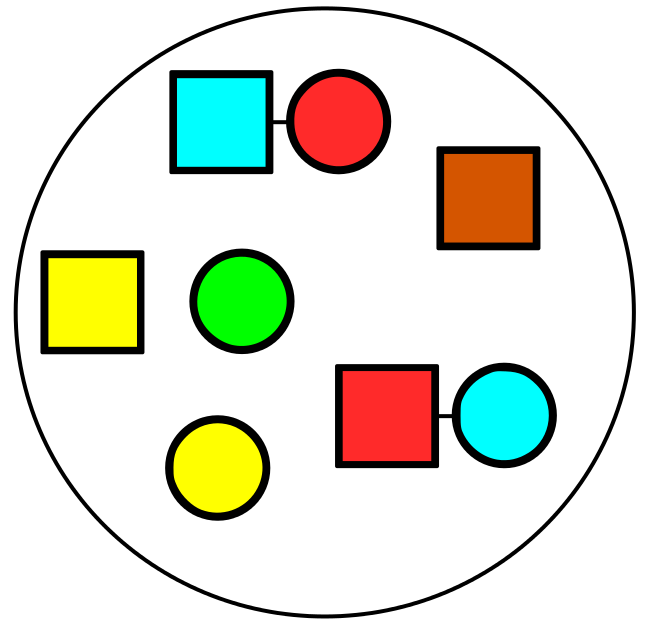
\includegraphics[scale=0.23]{pics/solution_first}\label{sol:s1}}
\hspace*{1cm}
\subfloat[]{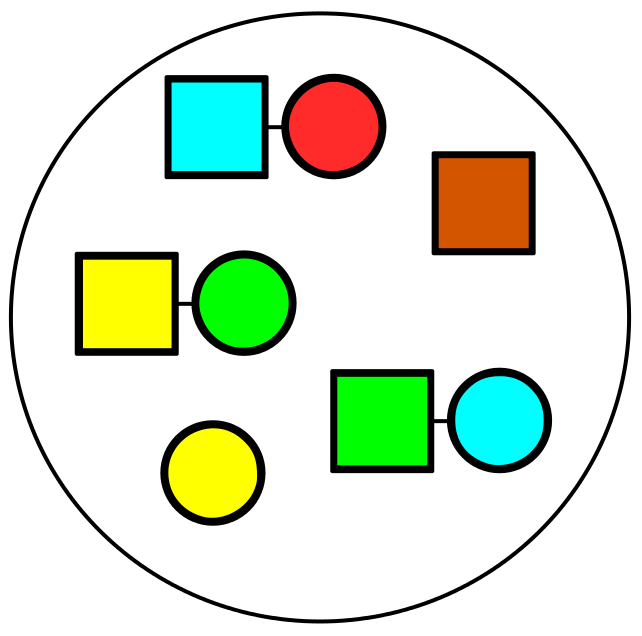
\includegraphics[scale=0.23]{pics/solution_second}\label{sol:s2}}
\end{center}
\caption{Examples of solutions. \textbf{(a)} An example of graphical representation of a solution. \textbf{(b)} Updated solution after the rules from Figure~\ref{rules:fig} were applied. The first rule \emph{(1)} was applied on the yellow {\large $\square$} and the green $\bigcirc$ and produced the yellow-green complex {\large $\square$}--$\bigcirc$. Note there are more options how the rule could be mapped -- each combination of free {\large $\square$} and $\bigcirc$. The second rule \emph{(2)} was applied on the red-cyan complex {\large $\square$}--$\bigcirc$ where the colour of {\large $\square$} was changed from red to green. The third rule \emph{(3)} couldn't be applied because there is no such complex with a yellow $\bigcirc$. }\label{solutions:fig}
\end{figure}

% replace all 
% {\large $\square$}
% to \raisebox{-0.02cm}[0cm]{{\large $\square$}}

\begin{figure}[!h]
\begin{center}
\begin{minipage}[l]{0.1\textwidth}
    \textbf{(1)}
  \end{minipage}
  \begin{minipage}[r]{0.6\textwidth}
    {\hspace*{0.8cm}
\includegraphics[scale=0.2]{pics/rule_complex}}
\end{minipage}

\begin{minipage}[l]{0.1\textwidth}
    \textbf{(2)}
  \end{minipage}
  \begin{minipage}[r]{0.6\textwidth}
    {\hspace*{1.35cm}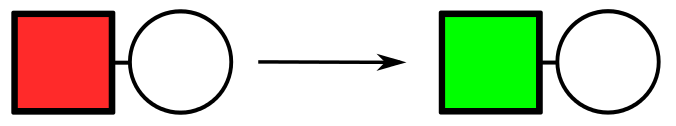
\includegraphics[scale=0.2]{pics/rule_change}}
\end{minipage}

\begin{minipage}[l]{0.1\textwidth}
    \textbf{(3)}
  \end{minipage}
  \begin{minipage}[r]{0.6\textwidth}
    {\hspace*{1.3cm}
\includegraphics[scale=0.2]{pics/rule_diss}}
\end{minipage}
\end{center}
\caption{Examples of rules. Rule \textbf{(1)}: a {\large $\square$} and a $\bigcirc$ can form a complex {\large $\square$}--$\bigcirc$ regardless their colours. Rule \textbf{(2)}: a {\large $\square$} is allowed to change its colour from red to green only if is in a complex with a $\bigcirc$ regardless its colour. Rule \textbf{(3)}: the rule can disassemble the complex only if the $\bigcirc$ is yellow.}\label{rules:fig}
\end{figure}

The rule is mapped on a solution. Then it can be applied and a new solution is produced. The mapping is not always successful (Figure~\ref{solutions:fig}, application of rule 3).

The mapping of a rule on a solution can be understood as a particular moment when the objects in the solution have just the conformation suitable for the rule and therefore the rule can be applied. Since the distribution of objects is random, we can assume a sequence of objects needed for rule (if there are such objects) is always available.

\begin{figure}[!h]
\begin{center}
\begin{minipage}[l]{0.1\textwidth}
    \textbf{(a)}
  \end{minipage}
  \begin{minipage}[r]{0.6\textwidth}
    {\hspace*{1.3cm}
\includegraphics[scale=0.2]{pics/rule_complex}}
\end{minipage}

\begin{minipage}[l]{0.1\textwidth}
    \textbf{(b)}
  \end{minipage}
  \begin{minipage}[r]{0.6\textwidth}
    {\hspace*{1.3cm}
\includegraphics[scale=0.2]{pics/rule_complex_mapped}}
\end{minipage}

\begin{minipage}[l]{0.1\textwidth}
    \textbf{(c)}
  \end{minipage}
  \begin{minipage}[r]{0.6\textwidth}
    {\hspace*{1.3cm}
\includegraphics[scale=0.2]{pics/rule_reaction}}
\end{minipage}
\end{center}
\caption{Example of a map-apply action. As a solution, we use the solution \emph{(a)} from Figure~\ref{solutions:fig}. \textbf{(a)} Rule can be mapped on a {\large $\square$} and a $\bigcirc$ regardless their colours and form a complex {\large $\square$}--$\bigcirc$.  \textbf{(b)} We randomly choose the yellow {\large $\square$} and the green $\bigcirc$ from our solution. The rule was mapped on chosen objects and they were assigned to the left-hand side of the rule. \textbf{(c)} The rule was applied and new object (the yellow-green complex {\large $\square$}--$\bigcirc$) was created. We obtained the reaction describing the particular action which has just happened.}\label{map-apply:fig}
\end{figure}

The mapping can also be seen as assigning particular objects from the solution to types on the left-hand side of the rule. The rule application then represents the change of the mapped objects to new objects according to the right-hand side of the rule (i.e., particular objects are assigned to the right-hand side). As a by-product, we obtain an instance of the rule -- a reaction (Figure~\ref{map-apply:fig}).

Since this kind of graphical representation is not very suitable for machine processing and analysis, we define a formal language which is built on principles described in this chapter.

\section{Rule-based vs. reaction-based modelling}

A rule is a generalised reaction (Figure~\ref{reaction_vs_rule}). This is how the difference can be characterised. From the application point of view, the reaction can be applied on a solution only in a particular way whilst the rule can be applied in multiple ways. It allows to write models where many similar processes might occur with the rules, by defining a pattern in which the action can happen. Since there can be many features we need to express, there are several languages focusing on different level of details.

\begin{figure}[!h]
\begin{center}
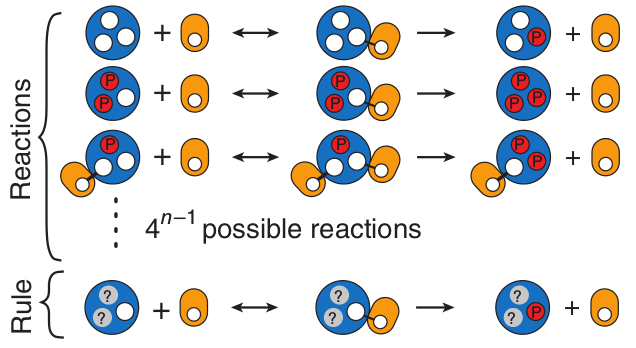
\includegraphics[scale=0.5]{pics/reaction_vs_rule}
\end{center}
\caption{Graphical comparison of the rule-based and the reaction-based approaches~\cite{sneddon2011efficient}. There can be seen combinatorial explosion in the number of possible particular interactions (the reactions), which can be depicted in a few simple rules.}\label{reaction_vs_rule}
\end{figure}

Analysing the rules directly is not the best choice. The main reason are \emph{side effects}, which might happen during the rule application. These side effects differ from language to language. There is no such thing for the reactions because the entire context is enumerated explicitly. Basically, we cannot directly know how exactly the rule will be used.

The rule and the reaction differ in the level of abstraction. In this context we mean how stringent it is, not what sort of features particular language uses. This is universal attribute for all rule-based languages -- the rule is always more abstract than its instance -- the reaction. The analysis of such abstract objects statically is a challenge. The reason is that most of the structural information is encoded in the rules implicitly. Explicit data are more suitable for static analysis.

\section{Rule-based languages}
\label{rule_based_languages}

There are several rule-based languages dedicated for modelling of the biological systems. Each of them uses different features and abstractions. In this chapter, we will highlight the key features for some representatives of them.

\subsection{Kappa language}
\label{kappa}

The Kappa language~\cite{kappa_formal} was primary developed for the modelling of protein interactions. The key structures used in the language are \emph{agents} with \emph{binding sites}, which allow formation of \emph{bonds} between the agents. Each binding site must be unique with at most one bond. Each site can occur in one of several pre-defined states.

The Kappa \emph{rules} are changing properties of the agents. Particularly, it might add, delete, or change a bond or a state of one or multiple agents at once. The rules are patterns with two sides where each of them is a sequence of agents delimited by a comma. Same as all the other rule-based languages, when some context is not relevant, it is omitted. Example of a rule is in Figure~\ref{kappa-rule}.

\begin{figure}[!h]
\begin{center}
\begin{tabular}{c l}
(a) & A(bsa$\sim$\{ u, p \}) ; B(bsb$\sim$\{ a, i \}) \\
(b) & A(bsa), B(bsb$\sim$a) $\rightarrow$ A(bsa!1), B(bsb$\sim$a!1) \\
\end{tabular}
\end{center}
\caption{Example of a Kappa rule. (a) Definition of associated agents. There are allowed two agents, A and B, both with a binding site which might occur in two possible states. (b) The rule itself. It defines creation of bond on the sites of agents A and B such that site of agent B must be in an active state. Note the context with no importance for the interaction is omitted.}\label{kappa-rule}
\end{figure}

The general problem they have to handle in the Kappa language is too detailed description. For biological systems as defined in Chapter~\ref{Rule-based basics}, it might be often hard to deal with all the bonds, especially in cases when we do not need such details.

\subsection{BioNetGen Language}
\label{bngl}

The BioNetGen Language (BNGL) \cite{BNGL} is very similar to the Kappa language and also has similar disadvantages. There are a few general differences: 

\begin{enumerate}
	\item it is allowed to define multiple binding sites with same name for an agent,
	\item one binding site is allowed to have multiple bonds,
	\item in the rules, BNGL uses `+' and `.' for expressing reaction complex and complex of agents respectively.
\end{enumerate}

Example of a rule is given in Figure~\ref{bngl-rule}.

\begin{figure}[!h]
\begin{center}
\begin{tabular}{c l}
(a) & A(bsa$\sim$u$\sim$p) \\
  & B(bsb$\sim$a$\sim$i) \\
(b) & A(bsa) + B(bsb$\sim$a) $\rightarrow$ A(bsa!1).B(bsb$\sim$a!1) \\
\end{tabular}
\end{center}
\caption{Example of a BNGL rule. (a) Definition of associated agents. There are allowed two agents, A and B, both with a binding site which might occur in two possible states. (b) The rule itself. Note the A and B agents must first create \emph{reaction complex} denoted by `+' (i.e., they must be close to each other) and then they create \emph{complex of agents} denoted by `.' (i.e., they are physically connected).}\label{bngl-rule}
\end{figure}

\subsection{Chromar}

The Chromar language~\cite{honorato2017chromar} allows to define attributes for agents and range them over pre-defined domains. The qualitative semantics are given by rule match on multisets composed of these agents producing a reaction. It is followed by standard application of the reaction (in manner of multiset operations). The language is very useful when creating a model where we need to create new distinct objects and control population of these objects.

Embedding this language to functional programming language Haskell increases its expressive power while making the ability of some analysis more expensive. Moreover, a user needs to understand Haskell (at least its basics) in order to use Chromar.

It is important to highlight a feature which stochastic semantics of this language offers. Compared to the other rule-based languages, it is capable of specifying rates for individual reactions inherited from the rule (Figure~\ref{chromar_rule}). It is allowed by variable value bindings and type-determination between left and right-hand side of the rule.

\begin{figure}[!h]
\begin{center}
A(a = x), A(a = y) $\xrightarrow[]{\text{f(x,y)}}$ A(a = x + y), A(a = y - 1) [g(x, y)]
\end{center}
\caption{Example of a Chromar rule. Arithmetic operations can be used in order to change properties of individual agents. Moreover, a rate function $f$ and conditional function $g$ increase applicability and practical use of the rule.}\label{chromar-rule}\label{chromar_rule}
\end{figure}

However, when it comes to readability and presentation to the user, the language is not a best choice. All the biologically relevant terms such as states have to be encoded in natural numbers.

\subsection{PySB}

The PySB language~\cite{Lopez646} works as a package in Python programming language. The definition of the models directly in the code allows to use the full syntax of Python, what significantly increases expression power of PySB. On the other hand, it might be hard to follow abstractions which are possible this way and models themselves are hard to analyse. Moreover, the core of the language is made by translating to BNGL (Section~\ref{bngl}). An example of a rule is given in Figure~\ref{pysb_rule}.

\begin{figure}[!h]
\begin{center}
\begin{python}
# Declare the monomers
Monomer('L', ['s'])
Monomer('R', ['s'])

# Declare the binding rule
Rule(L(s=None) + R(s=None) <> L(s=1) % R(s=1), kf, kr)
\end{python}
\end{center}
\caption{Example of a PySB rule. The rule describes creation of a bond between agents $\mathtt{R}$ and $\mathtt{L}$.}\label{PySB-rule}\label{pysb_rule}
\end{figure}

\subsection{SBML-multi package}

\begin{figure}[!h]
\lstset{language=XML}
\begin{lstlisting}[basicstyle=\scriptsize, frame=single]
<?xml version="1.0" encoding="UTF-8"?>
<sbml xmlns="http://www.sbml.org/sbml/level2" level="2" version="1">
  <model>
    <listOfCompartments>
      <compartment id="c" constant="true" multi:isType="true" />
      <compartment id="cc" constant="true" multi:isType="true">
        <multi:listOfCompartmentReferences>
          <multi:compartmentReference multi:id="cr1" multi:compartment="c" />
          <multi:compartmentReference multi:id="cr2" multi:compartment="c" />
        </multi:listOfCompartmentReferences>
      </compartment>
    </listOfCompartments>
    <multi:listOfSpeciesTypes>
      <multi:bindingSiteSpeciesType multi:id="stA" multi:compartment="c" />
      <multi:speciesType multi:id="stAA" multi:compartment="cc">
        <multi:listOfSpeciesTypeInstances>
          <multi:speciesTypeInstance multi:id="stiA1" multi:speciesType="stA"
            multi:compartmentReference="cr1" />
          <multi:speciesTypeInstance multi:id="stiA2" multi:speciesType="stA"
            multi:compartmentReference="cr2" />
        </multi:listOfSpeciesTypeInstances>
        <multi:listOfInSpeciesTypeBonds>
          <multi:inSpeciesTypeBond multi:bindingSite1="stiA1" multi:bindingSite2="stiA2" />
        </multi:listOfInSpeciesTypeBonds>
      </multi:speciesType>
    </multi:listOfSpeciesTypes>
    <listOfSpecies>
      <species id="spA" multi:speciesType="stA" compartment="c" ... />
      <species id="spAA" multi:speciesType="stAA" compartment="cc" ... />
    </listOfSpecies>
    <listOfReactions>
      <reaction id="reaction" ...>
        <listOfReactants>
          <speciesReference id="r1" species="spA" multi:compartmentReference="cr1" ... />
          <speciesReference id="r2" species="spA" multi:compartmentReference="cr2" ... />
        </listOfReactants>
        <listOfProducts>
          <speciesReference species="spAA" ... />
        </listOfProducts>
        ...
      </reaction>
      ...
    </listOfReactions>
  </model>
</sbml>
\end{lstlisting}
\caption{Example of a simple SBML-multi model. The model requires specification of language level (version). In the definition, there are included SpeciesTypes, Species which belong to these types, and Reactions where those species are interacting. Additionally, all processes are encapsulated in the compartments.}\label{SBML_example}
\end{figure}

Systems Biology Markup Language (SBML)~\cite{hucka2003systems} is a standard established for systems biology. A SBML-multi package~\cite{zhang2015sbml} is able to describe all the necessary rule-based features and therefore it is possible to export each model in a rule-based language in this format. It is the most suitable format for exchange and storage of the models but less for analysis and direct representation to the users (it is an XML format). It serves as an intermediate language.

\section{Comprehensive Modeling Platform}
\label{cmp}

Comprehensive Modeling Platform (CMP)~\cite{cs2bio2013} is an online platform providing tools for public sharing, annotation, analysis, and visualisation of dynamical models and \emph{wet-lab} experiments related to domain-specific systems. The platform is unique in integrating abstract mathematical models with a precise consortium-agreed biochemical description provided in a rule-based formalism. The general aim is to stimulate collaboration between experimental and computational systems biologists to achieve better understanding of the domain-specific system.

\begin{figure}[!h]
\begin{center}
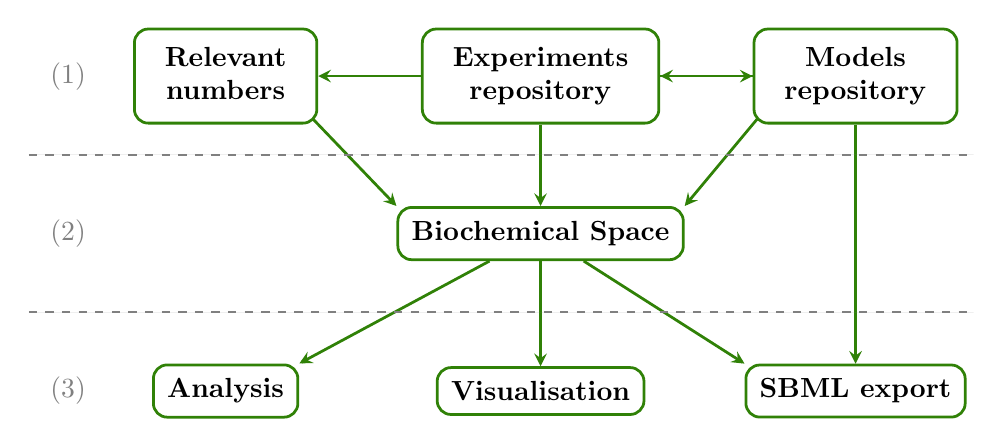
\begin{tikzpicture}[scale=1, transform shape, boxed/.style={rectangle, draw, line width=1pt, inner sep=5pt, rounded corners=5pt}]

% nodes ------------------------------------------------------------------------
\node [draw=mydarkgreen, boxed] (numbers) at (-2, 28) {\begin{tabular}{c}
                              \textbf{Relevant} \\
                              \textbf{numbers}
                          \end{tabular}};
\node [draw=mydarkgreen, boxed] (exper) at (2, 28) {\begin{tabular}{c}
                              \textbf{Experiments} \\
                              \textbf{repository}
                          \end{tabular}};
\node [draw=mydarkgreen, boxed] (models) at (6, 28) {\begin{tabular}{c}
                              \textbf{Models} \\
                              \textbf{repository}
                          \end{tabular}};

\node [draw=mydarkgreen, boxed] (bcs) at (2,26) {\textbf{Biochemical Space}};

\node [draw=mydarkgreen, boxed] (visual) at (2,24) {\textbf{Visualisation}};
\node [draw=mydarkgreen, boxed] (sbml) at (6,24) {\textbf{SBML export}};
\node [draw=mydarkgreen, boxed] (analysis) at (-2, 24) {\textbf{Analysis}};

\node [color=graybright] (1) at (-4, 28) {(1)};
\node [color=graybright] (2) at (-4, 26) {(2)};
\node [color=graybright] (3) at (-4, 24) {(3)};

% arrows ------------------------------------------------------------------------
\draw[myarrow, draw=mydarkgreen, fill=mydarkgreen, shorten <=-3pt, shorten >=1pt, line width=1pt] (numbers.south east) to (bcs.north west);
\draw[myarrow, draw=mydarkgreen, fill=mydarkgreen, shorten >=1pt, line width=1pt] (exper) to (bcs);
\draw[myarrow, draw=mydarkgreen, fill=mydarkgreen, shorten <=-3pt, shorten >=1pt, line width=1pt] (models.south west) to (bcs.north east);

\draw[myarrow, draw=mydarkgreen, fill=mydarkgreen, shorten >=1pt, line width=1pt] (models) to (exper);
\draw[myarrow, draw=mydarkgreen, fill=mydarkgreen, shorten >=1pt, line width=1pt] (exper) to (models);
\draw[myarrow, draw=mydarkgreen, fill=mydarkgreen, shorten >=1pt, line width=1pt] (exper) to (numbers);

\draw[myarrow, draw=mydarkgreen, fill=mydarkgreen, shorten >=1pt, line width=1pt] (bcs) to (visual);
\draw[myarrow, draw=mydarkgreen, fill=mydarkgreen, shorten >=1pt, line width=1pt] (bcs) to (analysis.north east);
\draw[myarrow, draw=mydarkgreen, fill=mydarkgreen, shorten >=1pt, line width=1pt] (bcs) to (sbml.north west);

\draw[myarrow, draw=mydarkgreen, fill=mydarkgreen, shorten >=1pt, line width=1pt] (models) to (sbml);

\draw[thick, dashed, draw=graybright, fill=graybright] (-4.5, 27) -- (7.5, 27);
\draw[thick, dashed, draw=graybright, fill=graybright] (-4.5, 25) -- (7.5, 25);
\end{tikzpicture}
\end{center}
\caption{An overview of Comprehensive Modeling Platform. It is composed of three layers: (1) input to the platform, all the relevant data; (2) Biochemical Space as an intermediate format for the data; (3) output of the platform, results of analysis and visualisation.}\label{cmp_overview}
\end{figure}

\subsection{Biochemical Space}
\label{bcs_general}

The platform consists of several dedicated modules (Figure~\ref{cmp_overview}), all connected to a central module -- \emph{Biochemical Space} (BCS)~\cite{BCS}, the backbone of the platform. BCS provides formal description and annotation of the biological system and it is based on the hierarchy of selected biological processes. It is accompanied with schemas representing relevant biological processes in the context of the modelled system. For each process, there are presented relevant models, chemical entities, and rules. Presentation of every process includes detailed information and links to the relevant internal and external sources.

BCS provides a well-described biological background for mathematical models of processes taking place in a specific organism. Complete BCS provides a connection between existing ontologies and mathematical models. BCS has a \emph{human-readable} format which can be easily edited in a dedicated editor and visualised within the platform. BCS is represented by two parts -- a set of \emph{entities} and a set of \emph{rules}.

When building the BCS, emphasis is put on well-defined and complete annotations. Links to the relevant ontologies must be specified for each entity and rule. Unique IDs provided by ontologies can help to automatically detect duplicities. IDs are also used to create hypertext links to related ontologies on the web, thus providing one part of the already mentioned connection between ontologies and models. At this moment, links to KEGG~\cite{Kanehisa04012016}, ChEBI~\cite{ChEBI}, CyanoBase~\cite{CyanoBase}, and other databases are supported (example of usage is in Figure~\ref{database_links}). A single entity or a rule can have multiple links to several external databases. An example is presence of a particular entity in ChEBI as well as in KEGG.

\begin{figure}[!h]
\begin{center}
\framebox{
{\footnotesize
\begin{tabular}{ l | l }
 DESCRIPTION: & Protein involved in N-acetylated amino acids hydrolysis\\
 LINKS: & \href{http://www.kegg.jp/dbget-bin/www_bget?ec:3.5.1.14}{KEGG::ec3.5.1.14}, \href{http://genome.microbedb.jp/cyanobase/GCA_000009725.1/genes/slr1653}{CBS::slr1653}, \href{http://genome.microbedb.jp/cyanobase/GCA_000009725.1/genes/sll0100}{CBS::sll0100}\\
 NOTES: & ChEBI link is missing
\end{tabular}}
}
\end{center}
\caption{Description, links, and notes information for an entity.}\label{database_links}
\end{figure}

The fact that most attributes in entity and rule definitions are tightly coupled with information from linked ontologies is the reason why we have started with describing annotation attributes. In the first place, one of these attributes is \emph{name}, which is taken from ontologies or follows the standard naming conventions. ID of every entity is fixed by the consortium. KEGG ID, ChEBI ID or internal ID is used if no reasonable ID is available. IDs of rules are internal.

\begin{figure}[!h]
\begin{center}
\framebox{
{\footnotesize
\begin{tabular}{ l | l }
 ENTITY ID: & HCO3\\
 STATES: & \{-, +\}\\
 LOCATIONS: & cyt, liq\\
 COMPOSITION:\\
 ENTITY NAME: & hydrogencarbonate\\
 CLASSIFICATION: & small molecule\\
 DESCRIPTION: & Plays major role in carbon concentrating\\
 & mechanism (CCM).\\
 LINKS: & \href{https://www.ebi.ac.uk/chebi/searchId.do?chebiId=17544}{CHEBI::17544}\\
 ORGANISM: & Synechococcus elongatus PCC 7942\\
\end{tabular}}
}
\end{center}
\caption{Complete information given for an atomic entity.}\label{entity_example}
\end{figure}

An entity in our interpretation is a bounded space (a so-called \emph{compartment}) or a structural part of a specific organism (for an example see Figure~\ref{entity_example}). BCS covers a hierarchy of \emph{entities} (or \emph{agents}) ranging from small molecules through composite structures to large complex molecules. Our goal is to make BCS as simple as possible. In existing ontologies, entities residing in several different states (oxidised, reduced, etc.) are usually treated as separate entities, thus causing the total number of entities to be enormous. To reduce this complexity, the concept of \emph{states} is defined in BCS. They enable definition of allowed set of states, in which an \emph{atomic} entity can occur.

BCS extends the traditional concept of the compartmentalisation with a hierarchy at the level of entities. A particular entity can reside in several different compartments. Additionally, \emph{classification} specifies the type of an entity in the sense of functional or structural characterisation.

An atomic entity can be a part of a structurally more complex entity. We consider two kinds of composite entities: \emph{structure} (Figure~\ref{structure_example}) and \emph{complex} entity. Structure entity represents partially specified composite species, for example a photosystem complex partially specified with prosthetic groups of interest. Complex entity represents fully specified composite species, for example, a homodimer of KaiC protein.

\begin{figure}[!h]
\begin{center}
\framebox{
{\footnotesize
\begin{tabular}{ l | l }
 ENTITY ID: & KaiC\\
 STATES:\\
 LOCATIONS: & cyt\\
 COMPOSITION: & S $|$ T\\
 ENTITY NAME: & circadian clock protein kinase KaiC\\
 CLASSIFICATION: & enzyme\\
 DESCRIPTION: & Monomer component representing a core component\\
 & of the circadian clock system.\\
 LINKS: & uniprot::Q79PF4, cyanobase::Synpcc7942\_1216\\
 ORGANISM: & Synechococcus elongatus PCC 7942
\end{tabular}}
}
\end{center}
\caption{Complete information given for a structure entity.}\label{structure_example}
\end{figure}

Rules are specified by \emph{rule equation} enriched with additional annotation information. When defining a rule equation, identifiers of substrates and products are used to make the notation of the rules compact. Every entity appearing in a rule equation has to be followed by the localisation operator associating it with a particular compartment. This is important especially for rules that act on both sides of a membrane. That way, a rule is always precisely localised in or between the compartments. A natural stoichiometric coefficient can be placed before any entity in a rule equation. Irreversible and reversible rules are distinguished by the operators `$\Rightarrow$', `$\Leftrightarrow$'. The `$+$' symbol is used as a separator between individual substrates and individual products. A rule can also have an assigned classification. Rule classification assigns a list of higher level biophysical processes in which the rule is involved. For an example, see Figure~\ref{rule_example}.

In some cases, emphasis on a detailed description leads to a very complex BCS models. Abstraction of some processes is needed to keep BCS models as simple as possible. To this end, rules expressing enzymatic reactions are considered in a simplified form. In fact, there should be at least two different rules describing an enzymatic reaction (one for a substrate binding and another for a catalytic step). Instead, since an enzyme is not affected during the reaction, it is affiliated to the rule as a \emph{modifier}. However, it is difficult to define precise meaning of a modifier in this case. We rather treat the modifier attribute informally as an entity \emph{which has to be present} for the rule to be enabled. The exact reaction mechanism of an enzyme is not always clear and therefore it is abstracted out.

\begin{figure}[!h]
\begin{center}
\framebox{
{\footnotesize
\begin{tabular}{ l | l }
 RULE ID: & FGFR2 phosph.\\
 RULE EQUATION: & $Thr\{u\}::FGF::FGFR2::cyt \Leftrightarrow $\\
 & $\Leftrightarrow Thr\{p\}::FGF::FGFR2::cyt$\\
 MODIFIER: & NDH1\\
 RULE NAME: & FGFR2 threonine residue (de)phosphorylation\\
 CLASSIFICATION: & phosphorylation, dephosphorylation\\
 DESCRIPTION: & FGF enzyme is phosphorylated on threonine residue\\
 & in FGFR2 complex.\\
\end{tabular}}
}
\end{center}
\caption{A rule employing structure entity state change. A Threonine ($Thr$) amino acid residue of a $FGF$ protein inside a $FGFR2$ complex can change its state from unphosphorylated ($u$) to phosphorylated ($p$) (and vice versa).}\label{rule_example}
\end{figure}

Higher abstraction comes into account when several electrons play `musical chairs' inside protein complexes. The issue is that parts of processing protein complex can have different unstable states during a short period of time. When one tries to define all rules among these proteins, combinatorial explosion of the number of states of the complex arises. Not all of these combinations are biologically correct. Even when excluding biologically inadmissible cases, the number of states is still enormous. For the purpose of BCS, we introduce a solution -- we treat a protein complex as a structure entity on which structurally simpler atomic entities change their states (not necessarily proteins) and we abstract out the background processes.

When describing particular process or object we can go almost infinitely deep into the details. Even if the depth is not infinite, it is deep enough to lead into state when the description is larger than object itself. Imagine that you want to describe a molecule as position of each atom. You definitely need more space to store such information than the molecule itself occupies.

When creating BCS for a system, we choose a level of details which we do not exceed. This ensures the size of BCS will not exponentially increase with additional details. The problem can occur when we try to map a model which uses more detailed description of the system than BCS does. However, we simply allow relating multiple model objects to BCS objects and vice versa. For example, multiple model reactions might be mapped on one BCS rule denoting the fact the process represented by the rule can be described in more details by the reactions. On the other hand, model might neglect some details. Then for example, a reaction can be mapped on multiple rules with similar meaning than in the previous case.

Since CMP allows export of models in SBML format, we employ resolvable identifier links~\cite{juty2011identifiers}. These links are included in generated SBML file and point to appropriate rules and entities in BCS.

\subsection{Model Repository}
\label{model}

The Model repository is a collection of implemented mathematical models describing particular parts of the biological processes. Each model is represented as a set of ordinary differential equations generated from the model reaction network. Models are integrated within BCS. In particular, each model component should be related to some BCS entity and each model reaction should be related to some BCS rule. The model is associated with some parameter value sets (\emph{data sets}) that enable simulation in a particular biologically-relevant scenarios. Additionally, several basic non-parameter-specific static analysis techniques based on model stoichiometry are also provided.

An implemented model then includes complete biological annotation of all components and reactions that is provided by mapping to BCS. This can help to find connections and overlaps among models. Further, implemented model can be exported to SBML.

\subsection{Experiments Repository}

The Experiments repository is a module for storage and presentation of time-series data from wet-lab experiments. Every experiment is well-grounded by precise description (device, medium, organism, etc.) and appropriate annotations. Experiments are structured -- several time series data can be attached to a single experiment. Every time series targets a specific list of measured substances together with time stamps of the individual measurements. Time series can be visualised in a chart.	

\chapter{Problem formulation}
\label{problem_formulation}

Biochemical Space as described in Section~\ref{bcs_general} can grow to enormous size. To be able to detect inconsistency with
automatic tools and enable further analysis of the space it is necessary to keep it on formal level.

%It means keep it consistent on an informal level is almost impossible. It is necessary to be able to detect inconsistency with automatic tools and enable further analysis of the space.

In our last paper~\cite{Ded201627}, we defined Biochemical Space Language (BCSL) such that syntax was defined independently, but semantics were defined via translating to Kappa language~\cite{kappa_formal}. We wanted to keep the language as concise as possible. The rule-based approach was the best choice, because it is capable to capture required details for biological systems while keeping the description concise. It was supposed to be \emph{human-readable}, which in this context means easy to read, write, and maintain by humans even from other disciplines than computer science. However, there are many rule-based languages, and each of them is slightly different on syntactic and semantic level and also on the level of abstraction. After a research (Section~\ref{rule_based_languages}), we have evaluated all existing languages as not suitable for our purposes. The closest representation to the desired one was Kappa language (Section~\ref{kappa}). That is the reason why in first version we have chosen translation to Kappa for definition of semantics.

However, this approach is not very beneficial since we are not fully using the expressive power of our language. The problem is Kappa operates purely on level of expressions. We want to promote our language to a higher level when it operates on objects in multisets. By translating to Kappa we loose such abstraction. 

In the previous version of language development, both definition and implementation were made via translation to Kappa. It particularly means there was defined a translation function, which was able to convert BCSL expressions to Kappa expressions. The huge advantage was that the conversion was quite straightforward and this way we could apply all types of analyses Kappa language offers.

The indirect approach had several disadvantages. Kappa has only one type of agent (no hierarchy). It follows all additional information encoded in different agent types are lost during the conversion. This particularly means atomic agents had to be considered as binding sites and structure agents as Kappa agents. But it was not always suitable, especially when atomic agents had an independent role in a rule. Complex treatment in Kappa requires explicit bonds between individual agents. Therefore, when translating our multiset-based complex agent to Kappa complex, we need to choose one of many possible isomorphisms (Figure~\ref{abstraction_comparision}, the biology corresponds to Kappa approach). Multiple default options are available, such as circular layout, linear layout etc. But it was not possible to express the fact that order does not matter.

\begin{figure}[!h]
\begin{center}
  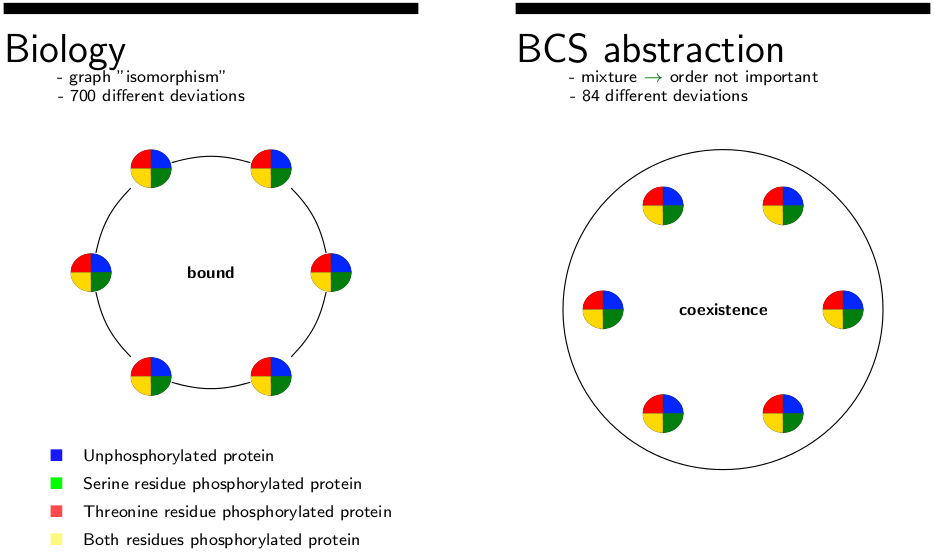
\includegraphics[scale=0.35]{pics/abstraction}
\end{center}
\caption{Comparison of a complex in biology (on the left) to abstraction used in BCS (on the right). In biology, all possible graph isomorphisms must be considered which results from combinatorial options how edges can be placed to create a connected graph~\cite{Chartrand1985} (additionally, we could consider the fact there might be multiple bonds between two entities). In BCS we neglect such details and see created structure only in the sense of coexistence (a multiset), which significantly reduces the number of possible derivations.}\label{abstraction_comparision}
\end{figure}

From the implementation point of view, executing models was delayed by the conversion to Kappa and then calling Kappa core to execute its semantics. Moreover, Kappa uses network-free simulator, which is very efficient for small models, because the rules are executed directly. Each rule is being matched on current state and then matched objects are replaced according to the rule. The problem is when the model is more complex. The number of rules does not cause any significant difference, however the number of interacting agents does. Once there are many agents, the time of one \emph{match \& replace} step rises dramatically. Compared to indirect methods when at first the reaction network is enumerated, the initial step can be resources consuming, but then the rule application itself is fast regardless the number of agents.

For the reasons mentioned above we decided to redefine the BCSL language. Particularly, the syntax definition had to be refined in order to make the usability more clear. From semantic point of view, we needed a straightforward definition, which would have practical use in implementation. Experience from previous versions showed that using direct rule-based semantics were not very efficient mechanisms. For that reason, we have chosen an indirect definition via translation to reactions -- \emph{practical} definition (Section~\ref{formal_definition}). The practical part means that this approach can be efficiently used in implementation.

In Section~\ref{bcs_general}, we have motivated the level of abstraction we need to use in BCS. To achieve that, we decided to neglect structural details, i.e. we do not employ binding approach. We consider binding as too low level of details. Instead, we improved definition of interacting agents to higher level, when an agent might expresses some kind of structural description (Figure~\ref{abstraction_comparision}). This way we avoid complicated creation of complexes and reduce complicated syntax.

Also, we determine two types of complexes. None of them is literally a complex, we rather see it as a coexistence. It allows us to express even other types of interaction. We also determine whether the expressed complex is complete, i.e. the enumerated subparts are all which form the complex. The other type of complex expresses the fact that subparts play an important role in the complex, but there are more parts which we do not model, but this fact is important for semantics of the model.

\chapter{Formal definition}
\label{formal_definition}

In this chapter, we define Biochemical Space Language formally. At first, we define all the required objects, then we define syntax of the language and semantics of the BCSL models.

The defined semantics is indirect, i.e. we do not give semantic sense to rules themselves, rather provide a procedure how to generate reactions from the rules and give semantics to them.

\section{Formal preliminaries}

Before we proceed, we provide some basic definitions and notations in order to build formal definition for the language.

%We define projection $\pi_i$ to enable iterating through multidimensional structures.

\begin{definition}{Multiset}
We define a \emph{multiset} $O$ as a pair $(A, \mathtt{m})$ where $A$ is some set and $ \mathtt{m} : A \rightarrow \mathbb{N} $ is a function from $A$ to the set of positive integers. The set $A$ is called the \emph{underlying set of elements}. For each $a$ in $A$ the \emph{multiplicity} (that is, number of occurrences) of a is the number $\mathtt{m}(a)$.
\end{definition}

\begin{notation}
Let $O = (A, m)$ be a multiset. By $x \in O$ we usually denote the fact that there exists $x \in A$ such that $m(x) \geq 1$.
\end{notation}

\begin{definition}{Projection}
\emph{Projection} $\pi_i : X^n \rightarrow X $ is defined as follows:

\begin{center}
$ \pi_i(x_1, \ldots, x_n) = $
  $\begin{cases}
  ~x_i & \ldots~~~~ 1 \leq i \leq n\\
  ~0 & \ldots~~~~ otherwise\\
  \end{cases}
  $
\end{center}
\end{definition}

\begin{definition}{Tuples concatenation}

Let $X = (x_1, \ldots, x_n), Y = (y_1, \ldots, y_m)$ be two tuples for some $n, m \in \mathbb{N}$. \emph{Concatenation} of two tuples, written $X \mdoubleplus Y$, is defined as:

\begin{center}
$X \mdoubleplus Y = (x_1, \ldots, x_n, y_1, \ldots, y_m)$.
\end{center}
\end{definition}

\begin{definition}{Sum of concatenations}

Let $T = (T_1, T_2, \ldots, T_n)$ be sequence of tuples. \emph{Concatenation} of sequence of tuples $\mdoubleplus_{i=1}^n T_i$ is defined as:

\begin{center}
$\mdoubleplus_{i=1}^n T_i = T_1 \mdoubleplus T_2 \mdoubleplus \ldots \mdoubleplus T_n $
\end{center}
\end{definition}

\begin{definition}{Non-crossing partition}
A partition $\mathcal{P} = B_1/B_2/\ldots/B_k$ of $S = [1,\ldots,n]$ is \emph{non-crossing} if  whenever a quadruple of elements $1 \leq a < b < c < d \leq n$ satisfies $a, c \in B_i$ and $b, d \in B_j$ for some $1 \leq i, j \leq k$, then in fact $i = j$; thus, the blocks do not cross.
\end{definition}

\begin{notation}
Let $\vv{v} = (x_1, \ldots, x_n)$ be a vector. By $\sigma(\vv{v})$ we denote set of all possible permutations of length $n$ of the vector $\vv{v}$.
\end{notation}

\begin{definition}{Labelled transition system}\label{lts}
\emph{Labelled transition system} (LTS) $\mathcal{L}$ is a quadruple $(S, A, T, s_0)$ where:

\begin{itemize}
  \item $S$ is a (potentially infinite) set of states (solutions),
  \item $A$ is a set of labels (reactions),
  \item $T \subseteq S \times A \times S$ is a transition relation (the map-apply action),
  \item $s_0 \in S$ is the initial state (initial solution).
\end{itemize}
\end{definition}

\begin{definition}{Path in LTS}
Let $\mathcal{L} = (S, A, T, s_0)$ be an LTS. We define \emph{path} as an finite sequence of states:

\begin{center}
$\mathtt{s}_1 \mathtt{s}_2 \ldots \mathtt{s}_n$
\end{center}

such that

\begin{center}
$\forall \mathtt{s}_i, \mathtt{s}_{i+1} : (\mathtt{s}_i, \mathtt{a}, \mathtt{s}_{i+1}) \in T$ for some $\mathtt{a} \in A$.
\end{center}

\end{definition}

\begin{definition}{Petri Net}
We define \emph{Petri Net} as a quadruple $\mathcal{N} = (P, T, F, m_0)$ where:

\begin{itemize}
	\item $P$ is a finite non-empty set of \emph{places},
	\item $T$ is a finite non-empty set of \emph{transitions},
	\item $F \subset ((P \times T) \cup (T \times P)) $ is a set of \emph{arcs},
	\item $m_0 : P \rightarrow \mathbb{N}$ is an initial \emph{marking}.
\end{itemize}
\end{definition}

\section{Objects definition}

Let $\mathcal{N}_{A}, \mathcal{N}_{T}, \mathcal{N}_{\delta}, \mathcal{N}_{c}$ be mutually exclusive finite sets of atomic names, structure names, states, and compartments respectively. Moreover, $\varepsilon$ is reserved symbol and does not belong to any of these sets.

For better readability, we provide examples of syntax for most important object with their definition. The formal definition of syntax and the relation to the objects will be given in subsequent sections.

\subsection{Signature}

\begin{definition}{Signature}
\emph{Atomic signature} $\Sigma_{\mathtt{A}} \subseteq \mathcal{N}_{A} \times 2^{\mathcal{N}_{\delta}}$ associates atomic names with set of state names. 

\emph{Structure signature} $\Sigma_{\mathtt{T}} \subseteq \mathcal{N}_{T} \times 2^{\mathcal{N}_{A}}$ associates structure names with set of atomic names. 
\end{definition}

Signatures define a set of allowed states for an atomic name and an allowed set of atomic names for a structure name. The deeper meaning will be revealed after next part of definitions.

\begin{example}{Signature}\label{example:signature}
\begin{itemize}
\item An atomic signature $\big\{~ (S, \{u, p\})$, $(Q, \{a, i\}) ~\big\}$
\item A structure signature $\big\{~ (KaiC, \{S, Q\}) ~\big\}$
\end{itemize}
\end{example}

\subsection{Atomic agent}

\begin{definition}{Atomic agent}
We define \emph{atomic agent} $\mathtt{A}$ as a pair $(\eta, \delta)$ where $\eta \in \mathcal{N}_{A}$ is a name and $\delta~\in~\mathcal{N}_{\delta} \cup \{ \varepsilon \}$ is a state.
\end{definition}

Atomic agents are the simplest objects used for describing biological entities. An atomic signature with the same name as the atomic agent defines all allowed states for it (with additional $\varepsilon$ state).

\begin{notation}
Let $\mathtt{A}$ be an atomic agent. We denote by $\eta(\mathtt{A})$ its name and by $\delta(\mathtt{A})$ its state.
\end{notation}

\begin{definition}{Equivalence of atomic agents}
Let $\mathtt{A},~ \mathtt{A}'$ be atomic agents. $\mathtt{A}$ is \emph{equivalent} to $\mathtt{A}'$, written $\mathtt{A} \equiv \mathtt{A}'$, \emph{iff} $\eta(\mathtt{A}) \equiv \eta(\mathtt{A}') \wedge \delta(\mathtt{A}) \equiv \delta(\mathtt{A}')$.
\end{definition}

\begin{notation}
We use symbol $\mathds{A}$ to denote the universe of all possible atomic agents.
\end{notation}

Universe $\mathds{A}$ represents all atomic agents which can be formed according to defined sets of atomic names and states.

Atomic agents are usually used to express small biological entities which can change their state, for example amino acids, small inorganic molecules etc.

\begin{example}{Atomic agents}\label{example:atomic}

\begin{itemize}
\item An atomic agent $\mathtt{A}_1 = (S, u)$
\begin{itemize}
	\item written as $S\{u\}$.
\end{itemize}
\item An atomic agent $\mathtt{A}_2 = (Q, \varepsilon)$
\begin{itemize}
	\item written as $Q\{\varepsilon\}$.
\end{itemize}
\end{itemize}
\end{example}

Note state $\varepsilon$ does not mean the agent is in \emph{none} state, but rather the state is unknown or not important.

\subsection{Structure agent}

\begin{definition}{Structure agent}
We define \emph{structure agent} $\mathtt{T}$ as a pair $(\eta, \gamma)$ where $\eta \in \mathcal{N}_{T}$ is a name and $\gamma \subseteq \mathds{A}$ is a set of atomic agents called partial composition.
\end{definition}

A structure agent represents a biochemical object that is composed of several known atomic agents while we know that a composition is abstract and not necessarily complete. To incorporate this kind of abstraction into our language, a structure agent is defined to be labelled with a unique name and it is constructed only from atomic agents considered in the same physical compartment.

\begin{notation}
Let $\mathtt{T}$ be a structure agent. We denote by $\eta(\mathtt{T})$ its name and by $\gamma(\mathtt{A})$ its partial composition.
\end{notation}

\begin{definition}{Equivalence of structure agents}
Let $\mathtt{T}, \mathtt{T}'$ be structure agents. $\mathtt{T}$ is \emph{equivalent} to $\mathtt{T}'$, written $\mathtt{T} \equiv \mathtt{T}'$, \emph{iff} $\eta(\mathtt{T}) \equiv \eta(\mathtt{T}') \wedge \gamma(\mathtt{T}) \equiv \gamma(\mathtt{T'})$.

%\forall \mathtt{A} \in \gamma(\mathtt{T}) ~\exists \mathtt{A}' \in \gamma(\mathtt{T}') : \mathtt{A} \equiv \mathtt{A}' \wedge \forall \mathtt{A}' \in \gamma(\mathtt{T}') ~\exists \mathtt{A} \in \gamma(\mathtt{T}) : \mathtt{A}' \equiv \mathtt{A}$.
\end{definition}

The key construct of a structure agent is \emph{partial composition} defined as a set of atomic agents which are considered to be relevant parts of the structure agent. We allow this set to be empty with the meaning of a biological structure for which we do not know its composition.

\begin{notation}
We use symbol $\mathds{T}$ to denote the universe of all possible structure agents.
\end{notation}

Universe $\mathds{T}$ represents all structure agents which can be formed according to defined sets of structure names w.r.t. universe of atomic agents.

A typical example of a structure agent is a protein where the atomic agents are individual amino acids that are of interest in the particular setting. For example,  imagine that in our system only three out of a few hundreds amino acids are able to undergo some post-translational modifications, such as phosphorylation, metylation etc. It is suitable to model only these three acids instead of entire primary structure of the protein.

\begin{example}{Structure agent}\label{example:structure}
\begin{itemize}
\item A structure agent $\mathtt{T}_1 = (K, \textcolor{red}{\{}(S, p), (Q, i)\textcolor{red}{\}})$
\begin{itemize}
	\item written as $K(S\{p\}, Q\{i\})$.
\end{itemize}
\item A structure agent $\mathtt{T}_2 = (K, \textcolor{red}{\{}(Q, a)\textcolor{red}{\}})$
\begin{itemize}
	\item written as $K(Q\{A\})$.
\end{itemize}
\end{itemize}
\end{example}

\subsection{Complex agent}

\begin{definition}{Complex agent}
We define \emph{complex agent} $\mathtt{X}$ as a pair $(\mu, \mathtt{com})$ where $\mu \in (\mathds{A} \cup \mathds{T})^n$ is a sequence of agents, $\mathtt{com} \in \mathcal{N}_{c}$ is a compartment, and $n \in \mathbb{N}$.
\end{definition}

A complex agent represents a non-trivial composite biochemical object that is inductively constructed from already known biological objects. In rule-based languages this is usually defined by introducing bonds between individual biochemical objects. In BCSL we abstract from detailed specification of bonds and we rather assume a complex as a coexistence of certain objects in a particular group. Moreover, a complex agent resides in a compartment which gives it a space position.

\begin{notation}
Let $\mathtt{X}$ be a complex agent. We denote by $\mu(\mathtt{X})$ its sequence of agents and by $\mathtt{com}(\mathtt{X})$ its compartment.
\end{notation}

\begin{definition}{Equivalence of complex agents}\label{rule_equiv}
Let $\mathtt{X}, \mathtt{X}'$ be complex agents. $\mathtt{X}$ is \emph{equivalent} to $\mathtt{X}'$, written $\mathtt{X} \equiv \mathtt{X}'$, \emph{iff} $|\mu(\mathtt{X})| \equiv |\mu(\mathtt{X'})| \wedge \mathtt{com}(\mathtt{X}) \equiv \mathtt{com}(\mathtt{X'}) \wedge \exists \mu' \in \sigma(\mu(\mathtt{X}'))$ such that $\forall i~\in~[1,~n]: \pi_i(\mu(\mathtt{X})) \equiv \pi_i(\mu')$ such that $n = |\mu(\mathtt{X})|$.
\end{definition}

The key element of a complex agent is \emph{sequence} describing inductively constructed coexistence expressions from existing agents. In contrast to partial composition in structure agent, we allow replication at the level of sequence (an agent of a certain name can appear more than once in a sequence).

\begin{notation}
We use symbol $\mathds{X}$ to denote the universe of all possible structure agents. Additionally, $\mathds{U}~=~\mathds{A}~\cup~\mathds{T}~\cup~\mathds{X}$ denotes universe of all possible agents.
\end{notation}

\begin{example}{Complex agent}\label{example:complex}

\begin{itemize}
\item A complex agent $\mathtt{X} = (\textcolor{green}{(}(K, \textcolor{red}{\{}(S, p), (Q, i)\textcolor{red}{\}}), (S, p)\textcolor{green}{)}, cytosol)$
\begin{itemize}
	\item written as $K(S\{p\}, Q\{i\}).S\{p\}::cytosol$
\end{itemize}
\end{itemize}
\end{example}

The complex agents encapsulate other agents -- an atomic or structure agent cannot exist on its own (there can be case when only one item is in its sequence). This guarantees each atomic and structure agent has indirectly given space location -- the compartment.

\subsection{Rule}

\begin{definition}{Rule}
\label{rule_definition}
We define \emph{rule} $\mathtt{R}$ as a quintuple $(\chi, \omega, \iota, \varphi, \psi)$ where:
\begin{itemize}
\item $\chi \in \mathds{X}^n$ is a sequence of complex agents,
\item $\omega \in (\mathds{A} \cup \mathds{T})^m$ is a sequence of atomic and structure agents,
\item $\iota \in \{ 0, \ldots, n \}$ is an index determining the end of left side of $\chi$,
\item $\varphi \in \mathbb{N}^m$ is an index map from $\omega$ to $\chi$,
\item $\psi \in ((\{-\} \cup \mathbb{N})^2)^n$ is an index map from left-hand side agents to right-hand side agents
\end{itemize}

where $n, m \in \mathbb{N}$.
\end{definition}

The reason for this particular definition of the rule is so-called \emph{practical} definition of semantics which can be seen in following sections. Also, it is necessary to capture relationship between left and right-hand side of the rule. This is done by enumerating all atomic and structure agents in $\omega$ and consequently creating index map between the agents in $\psi$. Another index map $\varphi$ serves for relating agents from $\omega$ back to original sequence of complexes $\chi$. Finally, by index $\iota$ we determine the end of left-hand side of the rule. Note the index is zero in the situation when we have no agents on the left-hand side.

\begin{notation}
We use symbol $\mathds{R}$ to denote the universe of all possible rules.
\end{notation}

\begin{example}{Rule}\label{example:rule}

\begin{itemize}
\item 
$\chi = \begin{bmatrix}
(\textcolor{green}{(} (K, \textcolor{red}{\{}(S, u)\textcolor{red}{\}}), (B, \textcolor{red}{\emptyset}) \textcolor{green}{)}, cyt),\\

(\textcolor{green}{(} (C, \textcolor{red}{\emptyset}), (D, i) \textcolor{green}{)}, cyt),\\

(\textcolor{green}{(} (A, \varepsilon) \textcolor{green}{)}, cyt),\\

(\textcolor{green}{(} (K, \textcolor{red}{\{}(S, p)\textcolor{red}{\}}), (B, \textcolor{red}{\emptyset}), (C, \textcolor{red}{\emptyset}) \textcolor{green}{)}, cyt),\\

(\textcolor{green}{(} (D, a), (A, \varepsilon) \textcolor{green}{)}, cyt),\\

(\textcolor{green}{(} (H, u) \textcolor{green}{)}, cyt)  
\end{bmatrix}$

\item $\omega = \begin{bmatrix}
(K, \textcolor{red}{\{}(S, u)\textcolor{red}{\}}), (B, \textcolor{red}{\emptyset}), (C, \textcolor{red}{\emptyset}), \\
(D, i), (A, \varepsilon), (K, \textcolor{red}{\{}(S, p)\textcolor{red}{\}}), \\
(B, \textcolor{red}{\emptyset}), (C, \textcolor{red}{\emptyset}), (D, a), (A, \varepsilon), (H, u)
\end{bmatrix}$

\item $\iota = 3$
\item $\varphi = (2,4,5,8,10,11)$
\item $\psi = [ (1,6) ; (2,7) ; (3,8) ; (4,9) ; (5,10) ; (-,11) ] $
\end{itemize}
 written as:

\begin{center}
\hspace*{-2cm}{\small $K(S\{u\}).B(\varnothing)::cyt + C(\varnothing).D\{i\}::cyt + A\{\varepsilon\}::cyt \Rightarrow$ 

$\Rightarrow K(S\{p\}).B(\varnothing).C(\varnothing)::cyt + D\{a\}.A\{\varepsilon\}::cyt + H\{u\}::cyt$}
\end{center}
\end{example}

Not every rule gives a sense. For example, a rule with no change or a rule with ambiguous relation of left and right-hand sides. In order to avoid such cases we need to specify when a rule is \emph{well-formed}, i.e. it gives semantically sense.

\begin{definition}{Well-formed rule}
Let $\mathtt{R}$ be a rule and $i,j \in \mathbb{N}$ natural numbers. We say the rule $\mathtt{R} = (\chi, \omega, \iota, \varphi, \psi)$ is \emph{well-formed} if the following conditions hold:

\begin{enumerate}
	\item \label{cond1} $\exists (i,j) \in \psi: \pi_i(\chi) \not\equiv \pi_j(\chi) $,
	\item \label{cond2} $\forall (i,j) \in \psi: \eta(\pi_i(\omega)) \equiv \eta(\pi_j(\omega))$.
\end{enumerate}

\end{definition}

A rule is well-formed if it does any action. It means, some change has to occur during rule application. This is ensured by condition~(\ref{cond1}), which requires at least one pair of complexes from left and right-hand side of the rule to be different. The second condition~(\ref{cond2}) has to hold on order to guarantee pairs of structure and atomic agents in $\omega$ of the rule have the same name. This condition is crucial for ground form function $\mathcal{G}$ defined in Section~\ref{ground_forms}, where adding context to different agents do not give a sense. 

Please note the conditions for well-formed rules do not apply on those agents which do not have a pair on the other side of the rule.

\subsection{Reaction}

\begin{definition}{Reaction}

We define \emph{reaction} $\mathtt{r}$ as a pair $(\mathtt{seq}, \iota)$ where:

\begin{itemize}
\item $\mathtt{seq} \in \mathds{X}^n$ is a sequence of complexes,
\item $\iota \in \{ 0, \ldots, n \}$ is an index determining start of right-hand side
\end{itemize}

where $n, m \in \mathbb{N}$.
\end{definition}

Reaction is similar structure than rule, but much simpler. The reaction is just mediate format for giving semantics to BCSL models and it only holds information about complex contents of the rule.

\begin{notation}
Let $\mathtt{r}$ be a reaction. We denote left-hand side of the reaction $(\pi_1(\mathtt{seq}), \ldots, \pi_{\iota}(\mathtt{seq}))$ as $LHS(\mathtt{r})$ and right-hand side of the reaction $(\pi_{\iota+1}(\mathtt{seq}), \ldots, \pi_{|\mathtt{seq}|}(\mathtt{seq}))$ as $RHS(\mathtt{r})$.
\end{notation}

\section{Syntax}
\label{syntax}

In Definition~\ref{grammar}, we provide grammar defining syntax of the BCSL. As proposed in Section~\ref{problem_formulation}, the syntax must be simple and readable. It was already defined in~\cite{Ded201627}, here we provide an improved and simplified version of the definition.

\begin{definition}{Grammar}
\label{grammar}
\begin{center}
\begin{tabular}{ l l }
atomic expression & $\alpha ::= \eta\{s\} ~|~ \eta\{\varepsilon\}$\\
 & $\eta ::= n \in \mathcal{N}_{A}$ \\
 & $s ::= n \in \mathcal{N}_{\delta}$\\
 & \\
structure expression & $\tau ::= \eta(\gamma) ~|~ \eta(\varnothing)$\\
 & $\gamma ::= \alpha_1, \ldots, \alpha_k$ \\
 & $\eta ::= n \in \mathcal{N}_{T}$\\
 & \\
complex expression & $\Gamma ::= \beta_1~.~\ldots~.~\beta_k :: c$\\
 & $\beta_i ::= \alpha ~|~ \tau$\\
 & $c ::= n \in \mathcal{N}_{c}$\\
 & \\
rule expression & $\varrho ::= \Gamma_1 + \ldots + \Gamma_n \Rightarrow \Gamma_{n+1} + \ldots + \Gamma_m $
\end{tabular}

\end{center}
where $m,n \in \mathbb{N}_0 \wedge m > n \wedge m + n \neq 0$ and $k \in \mathbb{N}$.
\end{definition}

Examples of syntax can be seen in the previous examples (Example~\ref{example:atomic} to \ref{example:rule}) and also in case study (Section~\ref{case_study}).

\section{BCSL model}
\label{BCSl_model}

When we have defined syntax of BCSL, we can proceed to BCSL model. We always consider initialised model, which means the definition contains an initial state of the system. The definition also contains rule expressions and signatures.

\begin{definition}{BCSL model}
\label{BCSL_model}
\emph{BCSL model} $\mathds{M}$ is a quadruple $(\mathcal{R}, \Sigma_\mathtt{A}, \Sigma_\mathtt{T}, \mathtt{init})$ where $\mathcal{R}$ is set of rule expressions, $\Sigma_\mathtt{A}$ is atomic signature, $\Sigma_\mathtt{T}$ is structure signature, and $\mathtt{init}$ is initial multiset of complex expressions.
\end{definition}

BCSL model is formed by a set of rule expressions $\mathcal{R}$, which define behaviour of the model. The initial multiset $\mathtt{init}$ defines the state of the model in the beginning. Atomic signature $\Sigma_\mathtt{A}$ define allowed states for all atomic agents used in the rules. Finally, structure signature $\Sigma_\mathtt{T}$ defines allowed atomic agents for all structure agents used in the rules.

\begin{remark}\label{BCS_vs_BCSL}
At this point it is useful to sum up what is Biochemical Space as described in Section~\ref{bcs_general} formally. The BCS is formed from a database of entities and rules. These entities are actually a signature, i.e. they predefine a domain on which rules can be defined. Neglecting an initial state (which is not relevant for entire space), the BCS is actually a BCSL model.

Additionally, BCS serves as a reference model for external kinetic models from Models repository. What we do in the process of relation is that we are actually assigning them BCSL notation. This way, smaller BCSL models are build with a reference to BCS. They inherit all annotation information provided by the reference model and gain formal representation of BCSL.
\end{remark}

\section{Additional definitions}

Before we proceed, there are a few necessary definitions. These definitions are required in next section in order to generate reactions from rules.

Reassembly operation $\Xi$ is quite a simple action on tuples. We need to reorganise tuple which has form $((a_1, b_1), (a_2, b_2), \ldots, (a_n, b_n))$ to a tuple of form $(a_1, a_2, \ldots, a_n, b_1, b_2, \ldots,  b_n)$. We define reassembly operation $\Xi$ generally on a set of tuples. 

\begin{definition}{Reassembly operation}

Let $Y$ be a set of tuples of particular form, where each $y \in Y$ has particular form $((a_1, b_1), (a_2, b_2), \ldots, (a_n, b_n))$. Then \emph{reassembly operation} $\Xi$ is defined as follows:

\begin{center}
$\Xi(Y) = \{~  x ~|~ y \in Y \wedge x = (\mdoubleplus_{i=1}^{|y|} \pi_1(y_i)) \mdoubleplus (\mdoubleplus_{i=1}^{|y|} \pi_2(y_i)) ~\}$
\end{center}
\end{definition}

We need to define difference of partial compositions of structure agents $\gamma \ominus \gamma'$. This difference is not just set difference, because we are not comparing atomic agents by overall equality, only equality on agent names. This operation is necessary in process of generating reactions from rules, which basically means adding details to partial compositions according to defined signatures.

\begin{definition}{Difference of partial compositions}

Let $\gamma, \gamma'$ be two partial compositions. We define \emph{difference of partial compositions} as follows:

\begin{center}
$\gamma \ominus \gamma' \myeq \{ \eta_\alpha ~|~ \exists \mathtt{A}: (\mathtt{A} \in \gamma \wedge \eta(\mathtt{A}) \equiv \eta_\alpha ) \wedge \not\exists \mathtt{A}': (\mathtt{A}' \in \gamma' \wedge \eta(\mathtt{A}') \equiv \eta_\alpha)\}$
\end{center}
\end{definition}

Similarly as in previous definition, we need to be able to find difference in context of atomic agent names between partial composition and structure signature.

\begin{definition}{Difference of partial composition and structure signature}

Let $\mathtt{T}$ be a structure agent, $\eta$ its name, and $\Sigma_T(\mathtt{T})$ appropriate signature. We define \emph{difference of partial composition} $\gamma(\mathtt{T})$ \emph{and structure signature} $\Sigma_T(\mathtt{T})$ as follows:

\begin{center}
$\Sigma_T(\mathtt{\eta}) \ominus \gamma(\mathtt{T}) \myeq \{ \eta_\Sigma ~|~ \eta_\Sigma \in \Sigma_T(\mathtt{\eta}) \wedge \not\exists \mathtt{A}: (\mathtt{A} \in \gamma(\mathtt{T}) \wedge \eta(\mathtt{A}) \equiv \eta_\Sigma)\}$
\end{center}
\end{definition}

The previous two definitions are very similar. The general difference is while in the first case we work purely with two partial compositions, in the second case we have a signature of appropriate structure agent name.

\section{Semantic function}
\label{semantic_function}

In the previous sections, we defined BCSL model using given syntax and BCSL objects with semantic meaning. Now, we need to connect them in order to we give semantic meaning to the model $\mathds{M}$. For this purpose, we define semantic function $\mathtt{F}$ (Definition~\ref{semantic_function}). It is defined recursively for a model $\mathds{M}$ according to expression given as an argument. 

\begin{definition}{Semantic function}
\label{semantic_function}
We define \emph{semantic function} $\mathtt{F}$ according to the expression given in double square brackets $\llbracket \ldots \rrbracket$ as follows:

\begin{center}
\begin{tabular}{ c c l}
$\mathtt{F} \llbracket ~\eta\{\varepsilon\}~ \rrbracket$ & = & $(\eta, \varepsilon) \in \mathds{A}$\\
 & & \\
$\mathtt{F} \llbracket ~\eta\{s\}~ \rrbracket$ & = & $(\eta, s) \in \mathds{A}$\\
 & & \\
$\mathtt{F} \llbracket ~\eta(\varnothing)~ \rrbracket$ & = & $(\eta, \emptyset) \in \mathds{T}$\\
 & & \\
$\mathtt{F} \llbracket ~\eta(\mathtt{a}_1, \ldots, \mathtt{a}_n)~ \rrbracket$ & = &
$(\eta, \{~ \mathtt{F} \llbracket \mathtt{a}_1 \rrbracket, \ldots, \mathtt{F} \llbracket \mathtt{a}_n \rrbracket ~\}) \in \mathds{T}$\\
 & & \\
$\mathtt{F} \llbracket ~\alpha_1~.~\ldots~.~\alpha_n :: c~ \rrbracket$ & = &
$(~(\mathtt{F} \llbracket ~\alpha_1~ \rrbracket, \ldots, \mathtt{F} \llbracket ~\alpha_n~ \rrbracket), ~c~) \in \mathds{X}$\\
 & & \\
$\mathtt{F} \llbracket ~\Gamma_1 + \ldots + \Gamma_n \Rightarrow \Gamma_{n+1} + \ldots + \Gamma_m~ \rrbracket$ & = &
$(\chi, \omega, \iota, \varphi, \psi) \in \mathds{R}$ :\\
\end{tabular}
\end{center}

\begin{center}
\begin{itemize}
\item $\chi = (\mathtt{F} \llbracket ~\Gamma_1~ \rrbracket, \ldots, \mathtt{F} \llbracket ~\Gamma_n~ \rrbracket, \mathtt{F} \llbracket ~\Gamma_{n+1}~ \rrbracket, \ldots, \mathtt{F} \llbracket ~\Gamma_m~ \rrbracket)$,
\item $\omega = \mdoubleplus_{i=1}^{|\chi|} \mu(\pi_i(\chi))$,
\item $\iota = n$,
\item $\varphi = (J_1, \ldots, J_m): J_k = \sum\limits_{i=1}^{k} | \mu(\pi_i(\chi)) |$,

\item \begin{tabular}{l l}

& \hspace*{-0.3cm} $\{~ (i,j) ~|~ i \in [1, \pi_\iota(\varphi)] \wedge j \in [\pi_{\iota}(\varphi) + 1, |\omega|] \wedge |i-j| \equiv \pi_\iota(\varphi)~\} ~\cup$ \\

\hspace*{-0.3cm}$\psi =$ & \hspace*{-0.3cm} $\{~ (i, -) ~|~ i \in [k, \pi_\iota(\varphi)] \wedge k = | \omega | - \pi_\iota(\varphi) + 1 ~| ~\} ~\cup$\\

& \hspace*{-0.3cm} $ \{~ (-, j) ~|~ j \in [k, |\omega|] \wedge k = 2 * \pi_{\iota}(\varphi) + 1 ~\}$
\end{tabular}

where $\psi$ is defined together with an ordering such that symbol $'-' > i$ for every $i \in \mathbb{N}$ and all descending intervals in definition of $\psi$ are ignored.

\end{itemize}
\end{center}
\end{definition}

Note by applying semantic function $\mathtt{F}$ on expressions from Examples~\ref{example:atomic} to \ref{example:rule}, we obtain agents (resp. rules) from appropriate examples. Moreover, semantic function works \emph{only} on BCSL object and rules well-defined by the given grammar (Section~\ref{syntax}).

\section{Ground forms}
\label{ground_forms}

\emph{Ground form} represents appending context to agents according to signature (we assume signature is always available and therefore we omit it in ground from function arguments). Particularly, this process means adding details to partial compositions and adding states of atomic agents according to defined signatures. Since there are typically multiple states allowed for an atomic agent, this processes leads to multiple options how to add a context. This is natural consequence of fact that a rule is an abstract representation of multiple reactions. 

\begin{definition}{Ground form function}
\label{ground_form}
We define \emph{ground form function} $\mathcal{G}$ for objects (middle column) of particular type (left column) as:

{\small
\begin{center}
\begin{tabular}{ c c c }
\textbf{Type} & \textbf{Notation} & \textbf{Ground form} \\
 & & \\
\hline
 & & \\
$\mathds{A}$ & $\mathcal{G}(\eta, \varepsilon)$ & $\{~ (\eta, \delta) ~|~ \delta \in \Sigma_A(\eta) ~\}$\\
 & $\mathcal{G}(\eta, \delta)$ & $\{~(\eta, \delta) ~\}$\\
 & & \\
  \hline
 & & \\
 $\mathds{A}^2$ & $\mathcal{G}(\mathtt{A}, \mathtt{A}')$ & $\{~ (a, a') ~|~ a \in \mathcal{G}(\mathtt{A}) \wedge a' \in \mathcal{G}(\mathtt{A}') \wedge \delta(a) \equiv \delta(a') ~\}$\\
 & & \\
 \hline
 & & \\
$\mathds{T}$ & $\mathcal{G}(\eta, \gamma)$ & $
  \Set{ (\eta, \gamma')\ | \begin{array}{l}
  \gamma' \equiv \gamma \cup \gamma_\Sigma \wedge \gamma_\Sigma \subseteq \mathcal{G}(\eta', \varepsilon) ~\wedge \\
  \wedge~ |\gamma_\Sigma| = |\Sigma_T(\eta) \ominus \gamma| \wedge \eta' \in \Sigma_T(\eta) \ominus \gamma \wedge\\
  \wedge~ \forall \widetilde{\eta} \in \Sigma_T(\eta) \ominus \gamma : \widetilde{\eta} \in  \gamma_\Sigma
  \end{array}}$\\
 & & \\
 \hline
 & & \\
$\mathds{T}^2$ & $\mathcal{G}(\mathtt{T}, \mathtt{T}')$ & $
  \Set{ (t, t')\ | \begin{array}{l}
  t \in \mathcal{G}(\mathtt{T}) \wedge t' \in \mathcal{G}(\mathtt{T}') ~\wedge \\
  \wedge~ \gamma(t) \ominus \gamma(\mathtt{T}) \equiv \gamma(t') \ominus \gamma(\mathtt{T}')
  \end{array}}$\\
  & & \\
 \hline
 & & \\
$\mathds{R}$ & $\mathcal{G}(\mathtt{R})$ & $ \displaystyle \prod_{k = 1}^{|\mathcal{G}(\psi)|} \mathcal{G}(\psi)_k $ \\ 
\end{tabular}
\end{center}

\noindent where $\mathcal{G}(\psi)_k = \mathcal{G}(\pi_i(\omega), \pi_j(\omega))$ such that $(i,j) = \pi_k(\psi)$ and $\mathtt{R} = (\chi, \omega, \iota, \varphi, \psi)$. Moreover, $\mathtt{A} = (\eta, \delta)$, $\mathtt{A}' = (\eta', \delta')$, $\mathtt{T} = (\eta, \gamma)$, and $\mathtt{T}' = (\eta', \gamma')$.
}
\end{definition}

In the Definition~\ref{ground_form}, objects (column \emph{notation}) of particular type (column \emph{type}) are transformed to their ground forms by ground form function $\mathcal{G}$ (column \emph{ground from}).

In case of single atomic agent $\mathtt{A}$, there are two options -- either the state is $\varepsilon$ or the state $\delta$ is given. In first case, we construct a set of all possible atomic agents according to the given atomic signature $\Sigma_A(\eta(\mathtt{A}))$. In the second case, we construct a set containing only the original agent itself.

For a pair of atomic agents $\mathtt{A}, \mathtt{A}'$ we create a set of all possible pairs $(a, a')$ such that these pairs has equal names.

Ground form of a structure agent $\mathtt{T}$ is a set of structure agents $\mathtt{T}'$ such that we \emph{insert} all neglected context information into its partial composition. In other words, we need to determine which atomic agents are missing in the partial composition, which can be obtained from the signature $\Sigma_T(\eta(\mathtt{T}))$. Then we create all possible combinations of inserted atomic agents recursively.

For a pair of structure agents $\mathtt{T}, \mathtt{T}'$ we expand both partial compositions recursively such that the expanded parts are equal, i.e. we add the same context to both agents. Similarly as in previous cases, we create set of all possibilities of such pairs.

Finally, ground form of a rule $\mathtt{R}$ is a Cartesian product of sets created for each pair of agents by applying ground from function. The pairs are given by order in index map $\psi$.

\section{Construction of reactions}
\label{Generating reactions}

Given a rule $\mathtt{R}$, we can produce appropriate reactions using ground forms and subsequent application of reassembly operation $\Xi$.

\begin{definition}{Construction of reactions}\label{generate_reactions}
\begin{center}
\begin{tabular}{ r@{\hskip 0.05cm}l }
$\mathtt{Reactions}(\mathtt{R}) =$ & $\{~ \mathtt{r}(\mathtt{seq}, \iota) ~|~ y \in \Xi(\mathcal{G}(\mathtt{R})) ~\}$\\

where $\mathtt{seq} =$ & $(\mathtt{X}_1, \mathtt{X}_2, \ldots, \mathtt{X}_n)$ such that\\

$\forall i \in [1, \ldots, n]: $ & $\mathtt{X}_i = \big( (\pi_{\varphi_{i-1}+1}(y), \ldots, \pi_{\varphi_i}(y)), \mathtt{com}(\pi_i(\chi)) \big)$\\

 & for $n = |\chi|$, $\varphi_0 = 0$, $ \iota \in \mathtt{R}$, $\chi \in \mathtt{R}$, $\varphi \in \mathtt{R}.$\\
\end{tabular}
\end{center}
\end{definition}

In Defintion~\ref{generate_reactions} we create the reassembled ground forms for a rule $\mathtt{R}$. Then, we create a set of reactions from created tuples of agents such that we preserve structure of original complex agents of rule $\mathtt{R}$. They are constructed using sequence of indices $\varphi$, which indicates the last positions in complex structures. In the case when for a particular complex agent $\mathtt{X}_i$ holds that $\pi_{\varphi_{i-1}+1}(y) = \pi_{\varphi_i}(y)$, the produced sequence $\mu$ is a singleton.

\section{Chemical reaction networks}

In this section, we define a simplified model that we can use to define operational semantics of BCSL model.

\begin{definition}{Chemical reaction model}
\label{crn}
\emph{Chemical reaction model} (CRM) $\mathcal{M}$ is a triple $(\mathfrak{R}, \vv{\nu}, \theta)$ such that $\mathfrak{R} \subseteq \mathbb{Z}^n$ is set of chemical reactions, $\vv{\nu} \in \mathbb{N}_0^n$ is initial vector, and $\theta \in \mathds{X}^n$ is vector of reference complexes for some $n \in \mathbb{N}$.
\end{definition}

Chemical reaction model is a simple model, where chemical reactions and initial state are vectors over integers. Moreover, there is a reference vector of complex agents, which serves for identification of the underlying agent on particular position in the vectors (chemical reactions).

\begin{notation}\label{nonnegative}
We denote $N(\vv{\mathtt{u}})$ condition $\forall i \in [1, \ldots, |\vv{\mathtt{u}}|]: \vv{\mathtt{u}}_i \in \mathbb{N}_0$.
\end{notation}

By Notation~\ref{nonnegative} we denote the condition that a vector is formed only by non-negative integers.

\begin{definition}{Chemical reaction application}

\emph{Chemical reaction application} $\zeta \subseteq \mathbb{N}_0^n \times \mathbb{Z}^n \times \mathbb{N}_0^n$ is a relation such that 
\begin{center}
$(\vv{\upsilon}, \vv{\mathtt{r}}, \vv{\mathtt{u}}) \in \zeta \myeq \vv{\mathtt{u}} = \vv{\upsilon} + \vv{\mathtt{r}} \wedge N(\vv{\mathtt{u}})$.
\end{center}
\end{definition}

Note some values in chemical reactions might be negative. When applying reaction on state, the resulting state cannot contain any negative values (negative number of entities does not give biological sense). Therefore, application is allowed only if the resulting vector contains non-negative values.

\begin{definition}{Semantics of chemical reaction model}
\label{states_creation}

Let $\mathcal{M} = (\mathfrak{R}, \vv{\nu}, \theta)$ be a chemical reaction model. The \emph{semantics of chemical reaction model} $\mathcal{M}$ are given in terms of the labelled transition system, $LTS(\mathcal{M})$, is defined as a quadruple $(S, A, T, s_0)$ such that:

\begin{enumerate}
	\item $ S $ is defined inductively:

	\begin{tabular}{l l}
	\emph{Basis}: & $\vv{\nu} \in S$\\
	\emph{Induction}: & $ \vv{\mathtt{s}} \in S \Rightarrow \forall \vv{r} \in \mathfrak{R}: \vv{\mathtt{p}} \in S $ such that $(\vv{\mathtt{s}}, \vv{\mathtt{r}}, \vv{\mathtt{p}}) \in \zeta $\\
	\end{tabular}
 
	\item $ A = \mathfrak{R} $,
	\item $ T = \{~ (\vv{\mathtt{s}}, \vv{\mathtt{r}}, \vv{\mathtt{p}}) ~|~ \vv{\mathtt{s}}, \vv{\mathtt{p}} \in S \wedge \vv{\mathtt{r}} \in \mathfrak{R}  \wedge (\vv{\mathtt{s}}, \vv{\mathtt{r}}, \vv{\mathtt{p}}) \in \zeta ~\} $,
	\item $ s_0 = \vv{\nu} $.
\end{enumerate}
\end{definition}

The quantitative semantics of model $\mathcal{M}$ are given in terms of a \emph{discrete-states} produced by inductive reaction application on initial vector $\vv{\nu}$ and all consequently created state vectors. This way we obtain an $LTS(\mathcal{M})$.

CRM semantics might lead to possibly infinite LTS. This process can be limited by a global bound, which makes sure the produced LTS is finite (Section~\ref{optimal_bound}).

\section{Construction of model}

In this section, we define relation between CRM and BCSL models and show how can their LTSs be translated to each other.

\begin{definition}{Reference vector}\label{reference_vector}

Let $\Theta$ be a set of all possible unique complexes constructed from reactions of model $\mathds{M}$ defined as follows:

$$\Theta = \{~ \mathtt{X} ~|~ \mathtt{X} \in \mathtt{seq}(\mathtt{r}) \wedge \mathtt{r} \in \bigcup_{\mathtt{R} \in \mathcal{R}} \mathtt{Reactions}(\mathtt{R}) ~\} $$

\noindent Then, the \emph{reference vector} $\theta$ is a tuple $X \in \Theta^n$ such that $\forall i,j \leq n : \Theta_i \not\equiv \Theta_j$ and $n~=~|\Theta|$. Note there are $n!$ possibilities how to choose $\theta$, an arbitrary one can be chosen.

\end{definition}

The reference vector enumerates all possible complex agents created for a model and assigns them a unique index. 

\begin{definition}{Multiset to vector translation}\label{state_to_vector}
\emph{Translation of a multiset} $\mathtt{S} \subseteq \mathds{X}$ \emph{to a vector} $(a_1, a_2, \ldots, a_n) \in \mathbb{N}^n$ is defined as follows:
\begin{center}
$\lambda(\mathtt{S}, \theta) = (a_1, a_2, \ldots, a_n)$ such that 
$a_i$ =
  $\begin{cases}
  |\mathtt{S}(\theta_i)| & \ldots~~~~ \theta_i \in \mathtt{S}\\
  0 & \ldots~~~~ \theta_i \not\in \mathtt{S}\\
  \end{cases}
  $
\end{center}
\hspace{15pt} where $n = |\theta|$ and $|\mathtt{S}(\pi_i)|$ is number of occurrences of agent $\pi_i$ in the multiset $\mathtt{S}$.
\end{definition}

Let $\mathds{M} = (\mathcal{R}, \Sigma_\mathtt{A}, \Sigma_\mathtt{T}, \mathtt{init})$ be a BCSL model. In order to construct chemical reaction model $\mathcal{M} = (\mathfrak{R}, \vv{\nu}, \theta)$ from the model $\mathds{M}$, we need to apply the following steps:

\begin{enumerate}
\item generate reactions for all rules $\mathtt{F}(\varrho) \in \mathcal{R}$ (Definition~\ref{generate_reactions}),
\item construct reference vector $\theta$ (Definition~\ref{reference_vector}),
\item create initial vector $\vv{\nu} = \lambda(\mathtt{S}, \theta)$ from initial multiset $\mathtt{S}$ where $\mathtt{S} = \{ \mathtt{X} ~|~ \mathtt{X} = \mathtt{F}(\Gamma) \wedge \Gamma \in \mathtt{init} \}$ (Definition~\ref{state_to_vector}),
\item construct set of chemical reactions $\mathfrak{R}$ from the set reactions, where individual vector reaction $\vv{r}$ is created from a reaction $\mathtt{r}$ as following:

\begin{center}
$\vv{r} = \lambda(RHS(\mathtt{r}), \theta) - \lambda(LHS(\mathtt{r}), \theta)$
\end{center}

\end{enumerate}

In Definition~\ref{states_creation} we show how to create an LTS from a chemical reaction model. In order to accomplish the process of giving semantics to an BCSL model, it is necessary to note how we revive information which is missing in produced LTS. This procedure is quite straightforward since we have defined reference vector $\theta$. Similarly as we translated multisets of BCSL agents to vectors (Definition~\ref{state_to_vector}), we can apply a reverse procedure, when we build a multiset of agents from a vector according to the reference vector $\theta$ (Definition~\ref{vector_to_state}).

\begin{definition}{Vector to multiset translation}
\label{vector_to_state}

\emph{Translation of a vector} $(a_1, a_2, \ldots, a_n) \in \mathbb{N}^n$ \emph{to a multiset} $\mathtt{S} = (A, \mathtt{m})$ is defined as follows:

\begin{center}
\begin{tabular}{r@{\hskip 0.05cm}l}
$\lambda^{-1}((a_1, a_2, \ldots, a_n), \theta) =$ & $ \mathtt{S}$ such that\\
$A = $ & $ \{~ \theta_i ~|~ i \in [1, \ldots, n] \wedge a_i > 0 ~\}$\\

$\mathtt{m} = $& $ \{~ (\theta_i, a_i) ~|~ i \in [1, \ldots, n] \wedge a_i > 0 ~\}$\\
& \\
where $n = |\theta|$. &\\
\end{tabular}
\end{center}
\end{definition}

The procedure provided in Definition~\ref{vector_to_state} can be extended to the labels of the LTS. The labels, which represent reactions applied, might contain negative numbers.

\begin{definition}{Negative part of vector to multiset translation}
\label{neg_vector_to_state}
Translation of the \emph{negative} part a vector $\mkern2mu\overline{\mkern-4.5mu \lambda^{-1}}$ is defined almost equally than the translation in Definition~\ref{vector_to_state} with exception that the condition $a_i > 0$ is modified to $a_i < 0$.
\end{definition}

% \begin{definition}{Negative vector to multiset translation}
% \label{neg_vector_to_state}
% Translation of the negative part a vector $(a_1, a_2, \ldots, a_n) \in \mathbb{N}^n$ to a multiset $\mathtt{S} = (A, \mathtt{m})$ is defined as follows:

% \begin{center}
% \begin{tabular}{r@{\hskip 0.05cm}l}
% $\mkern2mu\overline{\mkern-4.5mu \lambda^{-1}}((a_1, a_2, \ldots, a_n), \theta) =$ & $ \mathtt{S}$ such that\\
% $A = $ & $ \{~ \theta_i ~|~ i \in [1, \ldots, n] \wedge a_i < 0 ~\}$\\

% $\mathtt{m} = $& $ \{~ (\theta_i, |a_i|) ~|~ i \in [1, \ldots, n] \wedge a_i < 0 ~\}$\\
% & \\
% where $n = |\theta|$. &\\
% \end{tabular}
% \end{center}
% \end{definition}

The positive and negative parts of labels are treated independently. The negative numbers represent left-hand side of the reaction~ $\mkern2mu\overline{\mkern-4.5mu \lambda^{-1}}$ (the reactants) while positive numbers represent right-hand side of the reaction $\lambda^{-1}$ (the products).

\begin{definition}{LTS of BCSL model}
Let $\mathds{M} = (\mathcal{R}, \Sigma_\mathtt{A}, \Sigma_\mathtt{T}, \mathtt{init})$ be a BCSL model and $\mathcal{M} = (\mathfrak{R}, \vv{\nu}, \theta)$ be a chemical reaction model constructed from model $\mathds{M}$.

We define \emph{the labelled transition system of the BCSL model} $\mathds{M}$, $LTS(\mathds{M}) = (S, A, T, s_0)$, from the $LTS(\mathcal{M}) = (S', A', T', s'_0)$ such that:

\begin{center}
\begin{enumerate}
	\item $S = \{~ \mathtt{s} ~|~ \mathtt{s} = \lambda^{-1}(\mathtt{s}', \theta) \wedge \mathtt{s}' \in S' ~\}$,
	\item $A = \{~ (\mathtt{l}, \mathtt{r}) ~|~ \mathtt{l} = \mkern2mu\overline{\mkern-4.5mu \lambda^{-1}}(\mathtt{a}, \theta) \wedge \mathtt{r} = \lambda^{-1}(\mathtt{a}, \theta) \wedge \mathtt{a} \in A' ~\} $,

	\item $T = \Set{  (\mathtt{s}, (\mathtt{l}, \mathtt{r}), \mathtt{t})\ | \begin{array}{c}
      \mathtt{s} = \lambda^{-1}(\vv{\mathtt{s}}, \theta) \wedge \mathtt{t} = \lambda^{-1}(\vv{\mathtt{p}}, \theta) ~\wedge\\
      \wedge~ l = \mkern2mu\overline{\mkern-4.5mu \lambda^{-1}}(\vv{\mathtt{r}}, \theta) \wedge r = \lambda^{-1}(\vv{\mathtt{r}}, \theta) ~\wedge \\
      \wedge~ (\vv{\mathtt{s}}, \vv{\mathtt{r}}, \vv{\mathtt{p}}) \in T'
  \end{array}}$

	\item $s_0 = \lambda^{-1}(s'_0, \theta)$.
\end{enumerate}
\end{center}

\end{definition}

The LTS of a BCSL model is formed by states, labels, transitions, and an initial state. The states are multisets of complex agents, labels are individual reactions (the left and right-hand side multisets of complex agents respectively), and transitions are triples of (state, label, state) which represent edges. The initial state is a special state representing the origin of the system.

\section{Syntactic extensions}
\label{syntactic_extensions}

We define several syntactic extensions for better readability of the rule expressions. Note that each rule expression in an extended form can be always translated to basic form defined above. All rule expressions containing the following extensions must be converted to basic form before semantics can be applied.

For better demonstration we provide a running example, which will go through all syntactic extensions. Please note there is no biological sense of the model, it has only purpose to effectively demonstrate all defined syntactic extensions.

\begin{runningExample}{The example model $\mathds{M}$}
\label{run1}

\noindent Definition of rule expressions:
{\footnotesize
\begin{enumerate}
\item $KaiC(S\{u\}, T\{\varepsilon\}).KaiC(S\{\varepsilon\}, T\{\varepsilon\}).KaiC(S\{\varepsilon\}, T\{\varepsilon\})::cyt \Rightarrow $

$\Rightarrow KaiC(S\{p\}, T\{\varepsilon\}).KaiC(S\{\varepsilon\}, T\{\varepsilon\}).KaiC(S\{\varepsilon\}, T\{\varepsilon\})::cyt$

\item $KaiC(S\{u\}, T\{\varepsilon\}).KaiB::cyt \Rightarrow KaiC(S\{p\}, T\{\varepsilon\}).KaiB::cyt$
\item $KaiC(S\{\varepsilon\}, T\{\varepsilon\})::cyt + KaiC(S\{\varepsilon\}, T\{\varepsilon\})::cyt + KaiC(S\{\varepsilon\}, T\{\varepsilon\})::cyt \Rightarrow$ 

$ \Rightarrow KaiC(S\{\varepsilon\}, T\{\varepsilon\}).KaiC(S\{\varepsilon\}, T\{\varepsilon\}).KaiC(S\{\varepsilon\}, T\{\varepsilon\})::cyt$

\item $KaiC(S\{\varepsilon\}, T\{\varepsilon\}).KaiC(S\{\varepsilon\}, T\{\varepsilon\}).KaiC(S\{\varepsilon\}, T\{\varepsilon\})::cyt \Rightarrow $

$\Rightarrow KaiC(S\{\varepsilon\}, T\{\varepsilon\})::cyt + KaiC(S\{\varepsilon\}, T\{\varepsilon\})::cyt + KaiC(S\{\varepsilon\}, T\{\varepsilon\})::cyt$
\end{enumerate}
}

\begin{center}
\begin{tabular}{l@{\hskip 1.5cm}l}
Definition of $\Sigma_\mathtt{A}$: & Definition of $\Sigma_\mathtt{T}$:\\
1.~ $(S, \{ u, p \})$ & 1.~ $(KaiC, \{ S, T \})$\\
2.~ $(T, \{ a, i \})$ & 2.~ $(KaiB, \emptyset)$ \\
\end{tabular}
\end{center}

\noindent We omit $\mathtt{init}$ definition just for simplicity of the example.
\end{runningExample}

\subsection{Partial composition context elimination.}

It is possible to omit all atomic expressions with unspecified state $\varepsilon$ from partial compositions of structure agents. Such agent expressions do not give any additional information and whole partial composition can be reconstructed from the given signature.

\begin{runningExample}{The example model $\mathds{M}$}
\label{run2}

\noindent Definition of rule expressions:
{\footnotesize
\begin{enumerate}
\item $KaiC(S\{u\}).KaiC(\varnothing).KaiC(\varnothing)::cyt \Rightarrow KaiC(S\{p\}).KaiC(\varnothing).KaiC(\varnothing)::cyt$
\item $KaiC(S\{u\}).KaiB::cyt \Rightarrow KaiC(S\{p\}).KaiB::cyt$
\item $KaiC(\varnothing)::cyt + KaiC(\varnothing)::cyt + KaiC(\varnothing)::cyt \Rightarrow$

$ \Rightarrow KaiC(\varnothing).KaiC(\varnothing).KaiC(\varnothing)::cyt$
\item $KaiC(\varnothing).KaiC(\varnothing).KaiC(\varnothing)::cyt \Rightarrow$ 

$ \Rightarrow KaiC(\varnothing)::cyt + KaiC(\varnothing)::cyt + KaiC(\varnothing)::cyt$
\end{enumerate}
}
\end{runningExample}

Additionally, this extension can be done more precisely by omitting $(\varnothing)$ part completely. Since we have structure signature defined, we can unambiguously determine which names belong to structure expressions and this syntactic part can be easily reconstructed.

\begin{runningExample}{The example model $\mathds{M}$}
\label{run3}

\noindent Definition of rule expressions:
{\small
\begin{enumerate}
\item $KaiC(S\{u\}).KaiC.KaiC::cyt \Rightarrow KaiC(S\{p\}).KaiC.KaiC::cyt$
\item $KaiC(S\{u\}).KaiB::cyt \Rightarrow KaiC(S\{p\}).KaiB::cyt$
\item $KaiC::cyt + KaiC::cyt + KaiC::cyt \Rightarrow KaiC.KaiC.KaiC::cyt$
\item $KaiC.KaiC.KaiC::cyt \Rightarrow KaiC::cyt + KaiC::cyt + KaiC::cyt$
\end{enumerate}
}
\end{runningExample}

This syntactic extension brings a lot of readability to the syntax preserving all information in context of the model $\mathds{M}$.

\subsection{Complex signature}
\label{complex_signature}

We extend model definition by complex signature $\Sigma_\mathtt{X}$. In this signature, there are defined aliases for valid complex expressions. Then, simple \emph{replace} method is used to substitute original expression by the alias.

\begin{runningExample}{The example model $\mathds{M}$}
\label{run4}

\noindent Definitions of complex signatures:
\begin{enumerate}
\item $KaiC3::cyt = KaiC.KaiC.KaiC::cyt$
\item $KaiBC::cyt = KaiC.KaiB::cyt$
\end{enumerate}

\noindent Definition of rule expressions:
{\small
\begin{enumerate}
\item $KaiC(S\{u\}).KaiC.KaiC::cyt \Rightarrow KaiC(S\{p\}).KaiC.KaiC::cyt$
\item $KaiC(S\{u\}).KaiB::cyt \Rightarrow KaiC(S\{p\}).KaiB::cyt$
\item $KaiC::cyt + KaiC::cyt + KaiC::cyt \Rightarrow KaiC3::cyt$
\item $KaiC3::cyt \Rightarrow KaiC::cyt + KaiC::cyt + KaiC::cyt$
\end{enumerate}
}

\end{runningExample}

The usage of the complex signature has its limitations. Once a context is specified, the alias cannot be used. We will resolve this problem in following extensions.

\subsection{Directions}

We allow rule expressions to be bi-directional -- it is just a shortcut for two rule expressions and it can be converted to basic rule expression form. A rule expressions $\varrho : l ~\Leftrightarrow~ r$ could be written as two rule expressions $\varrho_1 : l ~\Rightarrow~ r$ and $\varrho_2 : r ~\Rightarrow~ l$.

\begin{runningExample}{The example model $\mathds{M}$}
\label{run5}
\noindent Definition of rule expressions:
{\small
\begin{enumerate}
\item $KaiC(S\{u\}).KaiC.KaiC::cyt \Rightarrow KaiC(S\{p\}).KaiC.KaiC::cyt$
\item $KaiC(S\{u\}).KaiB::cyt \Rightarrow KaiC(S\{p\}).KaiB::cyt$
\item $KaiC::cyt + KaiC::cyt + KaiC::cyt \Leftrightarrow KaiC3::cyt$
\end{enumerate}
}
\end{runningExample}

\noindent Definition of rules 3 and 4 from Running example~\ref{run4} was replaced by one bi-directional rule (Running example~\ref{run5}, rule 3).

\subsection{Stoichiometry}

For a rule expression of form 

\begin{center}
$\beta_1::\mathtt{c} + \beta_2::\mathtt{c} + \ldots + \beta_n::\mathtt{c} \Rightarrow \beta_1.\beta_2.~\ldots~.\beta_n::\mathtt{c}$
\end{center}

we might reorder both sides such that we get non-crossing partition $\mathcal{P} = B_1/B_2/\ldots/B_k$ from its indices $[1,\ldots,n]$ such that:

\begin{center}
$\forall B \in \mathcal{P}: \forall i,j \in B: \beta_i \equiv \beta_j$ 

and

$\forall B, B' \in \mathcal{P}: \forall \beta \in B ~\forall \beta' \in B': \beta \not\equiv \beta'$.
\end{center}

For the left-hand side $\beta_1::\mathtt{c} + \beta_2::\mathtt{c} + \ldots + \beta_n::\mathtt{c}$ of the reordered rule expression we can replace all rule expressions $[\beta_i, \ldots, \beta_j]$ which belong to the same non-crossing partition $B$ by notation $`k~\beta'$, where $\beta$ is a representative from $\beta_i, \ldots, \beta_j$ (they are all equivalent) and $k$ is number of the expressions in partition $B$.

Such a new rule expression is equivalent with the original rule expression what follows from the appropriate rules equivalence definition (Definition~\ref{rule_equiv}).

Note that this process is fully reversible -- we can simply enumerate all expressions for each partition.

\begin{runningExample}{The example model $\mathds{M}$}
\label{run6}
\noindent Definition of rule expressions:
{\small
\begin{enumerate}
\item $KaiC(S\{u\}).KaiC.KaiC::cyt \Rightarrow KaiC(S\{p\}).KaiC.KaiC::cyt$
\item $KaiC(S\{u\}).KaiB::cyt \Rightarrow KaiC(S\{p\}).KaiB::cyt$
\item $3~KaiC::cyt \Leftrightarrow KaiC3::cyt$
\end{enumerate}
}
\end{runningExample}

\noindent Definition of rule expression 3 from Running example~\ref{run5} was replaced by a new rule expression using stoichiometry.

\subsection{Locations}

Probably most complex syntactic extension is application of locations. The localisation operator is intended for allowing an alternative way of expressing the hierarchically constructed agent expressions. The main idea is to allow zooming into individual parts of complex and structure expressions.

We define necessary condition which must hold when semantic function $\mathtt{F}$ is applied on individual expressions. This notation is allowed only when the conditions hold. The condition is expressed using \emph{compatibility} operator defined in Section~\ref{static_analyses}.

\begin{definition}{Locations conditions.}\label{locations:conditions}

\begin{enumerate}
 \item $\mathtt{A}::\mathtt{T}$ $\Leftrightarrow$ there exists $\mathtt{A}' \in \gamma(\mathtt{T})$ such that $\mathtt{A} \lhd \mathtt{A}'$,

\item $\mathtt{A}::\mathtt{X}$ $\Leftrightarrow$ there exists $\mathtt{A}' \in \mu(\mathtt{X})$ such that $\mathtt{A} \lhd \mathtt{A}'$,

\item $\mathtt{T}::\mathtt{X}$ $\Leftrightarrow$ there exists $\mathtt{T}' \in \mu(\mathtt{X})$ such that $\mathtt{T} \lhd \mathtt{T}'$.
\end{enumerate}
\end{definition}

For each pair of agents $(\alpha, \beta)$ with allowed `::' operator between them $\alpha :: \beta$, we can construct just one agent $\beta'$ without the operator by taking the most left agent $\alpha'$ from full (resp. partial) composition of the agent $\beta$ such that it is \emph{compatible with} the agent $\alpha$ ($\alpha' \lhd \alpha$). Then, agent $\alpha'$ is simply replaced by agent $\alpha$ and agent $\beta'$ is constructed.

\begin{runningExample}{The example model $\mathds{M}$}
\label{run7}
\noindent Definition of rule expressions:
{\small
\begin{enumerate}
\item $S\{u\}::KaiC::KaiC3::cyt \Rightarrow S\{p\}::KaiC::KaiC3::cyt$
\item $S\{u\}::KaiC::KaiBC::cyt \Rightarrow S\{p\}::KaiC::KaiBC::cyt$
\item $3~KaiC::cyt \Leftrightarrow KaiC3::cyt$
\end{enumerate}
}
\end{runningExample}

\noindent Definition of rule expressions 1 and 2 from Running example~\ref{run6} was replaced using locations.

You can see localisation operator allowed us to fully use the complex signatures.

\subsection{Variables}

In the Running example~\ref{run7} there are additional options for syntax reduction. Rule expressions 1 and 2 are very similar except context of complex expression they take place in. Therefore, we will substitute this context with a variable with a given domain.

In a rule expression, one rule agent expression might be referenced using variable $\upsilon$ as a set of rule agent expressions it can be replaced with. Such a rule agent expression is referenced as $?X$. Moreover, in case when a $?X$ is used in a location, it must hold conditions from Definition~\ref{locations:conditions}.

Each rule expression associated with variable can be easily rewritten as several rule expressions where variable is replaced with agent expression from set of agent expressions attached to the variable. For simplicity, only one variable can be used per rule expression.

\begin{runningExample}{The example model $\mathds{M}$}
\label{run8}
\noindent Definition of rule expressions:
{\small
\begin{enumerate}
\item \hspace*{-0.6cm} $S\{u\}::KaiC::~?X::cyt \Rightarrow S\{p\}::KaiC::~?X::cyt ~;~ ?X = \{KaiC3, KaiBC\}$

\item \hspace*{-0.6cm} $3~KaiC::cyt \Leftrightarrow KaiC3::cyt$
\end{enumerate}
}
\end{runningExample}

\noindent Definition of rule expressions 1 and 2 from Running example~\ref{run7} was replaced as a single rule expression with a variable.

This is final syntactic extension. Compared to the original model (Running example~\ref{run1}), the resulting model is more concise and readable. More examples are in Section~\ref{case_study}.

\chapter{Analysis}
\label{analysis}

In the previous chapters, we defined BCS language. From the provided examples and case study (Section~\ref{case_study}) it should be clear that it provides concise and readable notation when it comes to describing biological systems. Moreover, accompanied with relevant annotation information, it is suitable for building huge models.

However, descriptive properties are not enough for using computational methods in order to analyse particular processes. In this chapter we describe basic approaches we employ for our language and propose several methods which could be potentially used in context of static analysis.

We distinguish two general approached in model analysis -- dynamic and static. Dynamic analysis is enabled by some form of executing the model. It requires either enumerating all possible scenarios of behaviour of a model (called \emph{state space}) or applying assumptions in order to calculate an average behaviour (such as simulation). Static analysis provides information without execution of the model, just by investigating its structure. Both approaches require to build particular mechanisms which enable application of the analysis.

\section{Dynamic analysis}

Dynamic analysis is a very common way how to analyse models written in formal representations. There are several types of analyses and they are usually trying to predict behaviour of the modelled system using formal description of the system -- the model.

\subsection{Model checking}

Model checking is an approach of checking whether given model meets a given specification~\cite{clarke1999model}. Typically this is done by specifying given requirements in a temporal logic formula and then check whether a given structure satisfies the formula. There are two version of model checking -- explicit-state and symbolic.

We will not discuss this approach any further since we have given semantics to the BCSL models, which are able to generate LTS (Definition~\ref{lts}). It is suitable for model checking analysis and can be applied in external tools including temporal properties specification.

Reachability analysis is a particular task of model checking for determining whether a chosen state is reachable in the LTS of a model.

\begin{definition}{Reachability relation}
\label{reachability_relation}
For an LTS $\mathcal{L} = (S, A, T, s_0)$ the \emph{reachability relation} of $\mathcal{L}$ is the transitive closure of $T$, which is a of all ordered pairs $(s,t)$ of states in $S$ for which there exists a sequence of states $s = s_0, s_1, s_2, \ldots, s_k = t$ such that the transition $(s_{i-1}, a, s_i)$ is in $T$ for all $1 \leq i \leq k$ and for some $a$ in $A$.
\end{definition}

In our case, reachability analysis can be generalised to checking whether for some multiset of complex agents $\mathtt{s}'$ there exists a reachable state $s \in S$ of an LTS $\mathcal{L}$ such that $\mathtt{s}' \subseteq s$. In other words, we are interested only in particular agents regardless other context in the reachable state. This might generally lead to multiple reachable states and then we can for example consider a shortest path.

In the case when we consider reachability \emph{only} from the initial state $s_0$, the task becomes simpler. The reason is all other states are actually reachable, because the entire state space was generated from this state. Then we are only searching for a state $s \in S$ such that $\mathtt{s}' \subseteq s$ if we are not interested in \emph{how} was the state reached (the particular path).

\subsection{Simulation}
\label{simulation}

Computer simulations reproduce the behaviour of a system using a mathematical model. For the purpose of this thesis, the simulation is a numerical solution which tries to mimic the behaviour of the real system over time. Once we want to simulate BCSL model, regardless the approach we choose, it is necessary to enrich the rules by kinetic rates~\cite{mcnaught1997compendium}. The rates basically express the speed of the rule.

Assigning a rate to the rule is not a simple task. The simplest solution is to reference only fully defined objects in the kinetic rates. However, we would like to express the context of the rule also in the rate. That typically means changing context in rate and the rule accordingly. This approach is non-trivial and we keep it as a future work.

Assigning rates to the rules enables deterministic simulation~\cite{Poole2000} by translating rules to reactions and consequently construct Ordinary Differential Equations (ODEs) from them~\cite{higham2008modeling}. It is possible to enable also stochastic simulation, either by network-free simulators such as NFsim~\cite{sneddon2011efficient} or using indirect approach on generated reactions (e.g. Gillespie algorithm~\cite{GILLESPIE1976403}).

\section{Static analysis}
\label{static_analyses}

The BCS language offers interesting capabilities in order to provide static analysis of given models. We define \emph{compatibility} operator $\lhd$ for each type of agents, which will help us to formulate properties suitable for static analysis.

\begin{definition}{Compatibility of atomic agents}
Let $\mathtt{A}_1$, $\mathtt{A}_2$ be atomic agents. The agent $\mathtt{A}_1$ is \emph{compatible with} agent $\mathtt{A}_2$, written $\mathtt{A}_1 \lhd \mathtt{A}_2$, if either $\mathtt{A}_1 \equiv \mathtt{A}_2$ or $\eta(\mathtt{A}_1) \equiv \eta(\mathtt{A}_2) \wedge \delta(\mathtt{A}_1) \equiv \varepsilon $.
\end{definition}

Note that compatibility of two atomic agents is very close to their equivalence. Additionally the left-hand side agent is allowed to have its state undefined while the state of right-hand side agent differs. 

\begin{definition}{Compatibility of structure agents}
Let $\mathtt{T}_1, \mathtt{T}_2$ be structure agents. The agent $\mathtt{T}_1$ is \emph{compatible with} agent $\mathtt{T}_2$, written $\mathtt{T}_1 \lhd \mathtt{T}_2$, \emph{iff} either $\mathtt{T}_1 \equiv \mathtt{T}_2$ or $\eta(\mathtt{T}_1) \equiv \eta(\mathtt{T}_2) \wedge \forall \mathtt{A}_1 \in \gamma(\mathtt{T}_1) ~\exists \mathtt{A}_2 \in \gamma(\mathtt{T}_2)$ : $\mathtt{A}_1 \lhd \mathtt{A}_2$.
\end{definition}

Structure agents are compatible if we are able to create pairs from atomic agents of composition of left-hand side agent with the right-hand side ones such that these atomic agents are all unique. For such pairs, the agents in each pair must be compatible.

\begin{definition}{Compatibility of complex agents}
Let $\mathtt{X}_1$, $\mathtt{X}_2$ be complex agents. The agent $\mathtt{X}_1$ is \emph{compatible with} agent $\mathtt{X}_2$, written $\mathtt{X}_1 \lhd \mathtt{X}_2$, \emph{iff} either $\mathtt{X}_1 \equiv \mathtt{X}_2$ or $\mathtt{com}(\mathtt{X}_1) \equiv \mathtt{com}(\mathtt{X}_2) \wedge \exists \mu' \in \sigma(\mu(\mathtt{X}_2))$ such that $ \forall i \in [1, n] : \pi_i(\mu(\mathtt{X}_1)) \lhd \pi_i(\mu') $, where $n$ is length of sequence which is the same for both sequences.
\end{definition}

Complex agents are compatible if there exists a permutation of sequence of the first agent such that individual agents on the same position in both sequences are compatible.

The insight from the previous chapters is that an agent might have its ancestors and successors. The compatibility operator formulates this relationship formally. Each successor is compatible with its ancestor, but the reverse relation does not hold. The successor has always more details specified.

\begin{notation}
Let $x, y$ be two agents. We denote $x \Delta y$ the fact the agents are compatible \emph{iff} either $x \lhd y$ or $y \lhd x$ holds.
\end{notation}

\begin{definition}{Partial order of agents}
\label{partial_order}
Let $x_1, x_2 \in P$ be agents and $P$ a universe of agents. Agents $x_1$ and $x_2$ are in \emph{partial order} relation, written $x_1 \leq x_2$, \emph{iff} $ x_1 \lhd x_2 $.
\end{definition}

\begin{notation}
The universe of complex agents $\mathds{X}$ ordered by partial order reduction $\leq$ is denoted as $\mathds{X}_\leq$.
\end{notation}

The compatibility operator generates partial order of $\mathds{A}, \mathds{T}$, and $\mathds{X}$ sets. For our purposes, partially ordered set $\mathds{X}_\leq$ is relevant. The reason is that complex agents actually encapsulate all other agent types including compartments. However, partial order of entire universe of complex agents is not very useful, since most of agents cannot be compared. We are interested in particular subsets which are formed from all complexes of the same type, i.e. those sets where each pair of complexes holds the compatibility conditions (in arbitrary direction).

\begin{definition}{Compatible set}
\label{compatible_set}
A finite set $\mathscr{X} \subseteq \mathds{X}$ is a \emph{compatible set} if:
\begin{center}
\begin{enumerate}
	\item \label{compatible_cond} $ \forall \mathtt{X}_1, \mathtt{X}_2 \in \mathscr{X} ~\exists~ \mathtt{X}' \in \mathscr{X}: \mathtt{X}_1 \lhd \mathtt{X}' \wedge \mathtt{X}_2 \lhd \mathtt{X}'$ such that $\mathtt{X}_1 \neq \mathtt{X}_2$,

 and for each finite set $\mathscr{X}' \subseteq \mathds{X}$ such that $\mathscr{X} \neq \mathscr{X}'$ holds:

	\item \label{non_compatible_cond} $\forall \mathtt{X} \in \mathscr{X} \forall \mathtt{X}' \in \mathscr{X}': \neg (\mathtt{X} ~\Delta~ \mathtt{X}') $.
\end{enumerate}
\end{center}

\end{definition}

\begin{remark}
\label{order_in_compat_set}
The compatible set $\mathscr{X}$ inherits partial order relation defined on $\mathds{X}_\leq$, which follows from conditions (\ref{compatible_cond}) and (\ref{non_compatible_cond}) of Definition~\ref{compatible_set}.
\end{remark}

A compatible set $\mathscr{X}$ contains partially ordered complex agents. Assuming we ignore states of individual atomic agents (including those inside partial compositions of structure agents), these complex agents are all equal. In other words, they all contain the same sequence of agent names. Example of a compatible set is given in Figure~\ref{compatible_set_example}.

\begin{lemma}
\label{global_supremum}
In every compatible set $\mathscr{X}$, there always exists a global supremum $\mathtt{sup}(\mathscr{X})$, what is an ancestor of all the remaining agents in the set (Remark~\ref{order_in_compat_set}).
\end{lemma}

\begin{proof}
The lemma follows from Definition~\ref{compatible_set} condition~(\ref{compatible_cond}) which basically claims that there is a supremum (in manner of compatibility) for each two complex agents in the compatible set $\mathscr{X}$. Since there exists a supremum for every two items in the set and the set is finite, there must exists a global supremum for the entire set. $\QEDA$
\end{proof}

\begin{figure}[!h]
\begin{center}
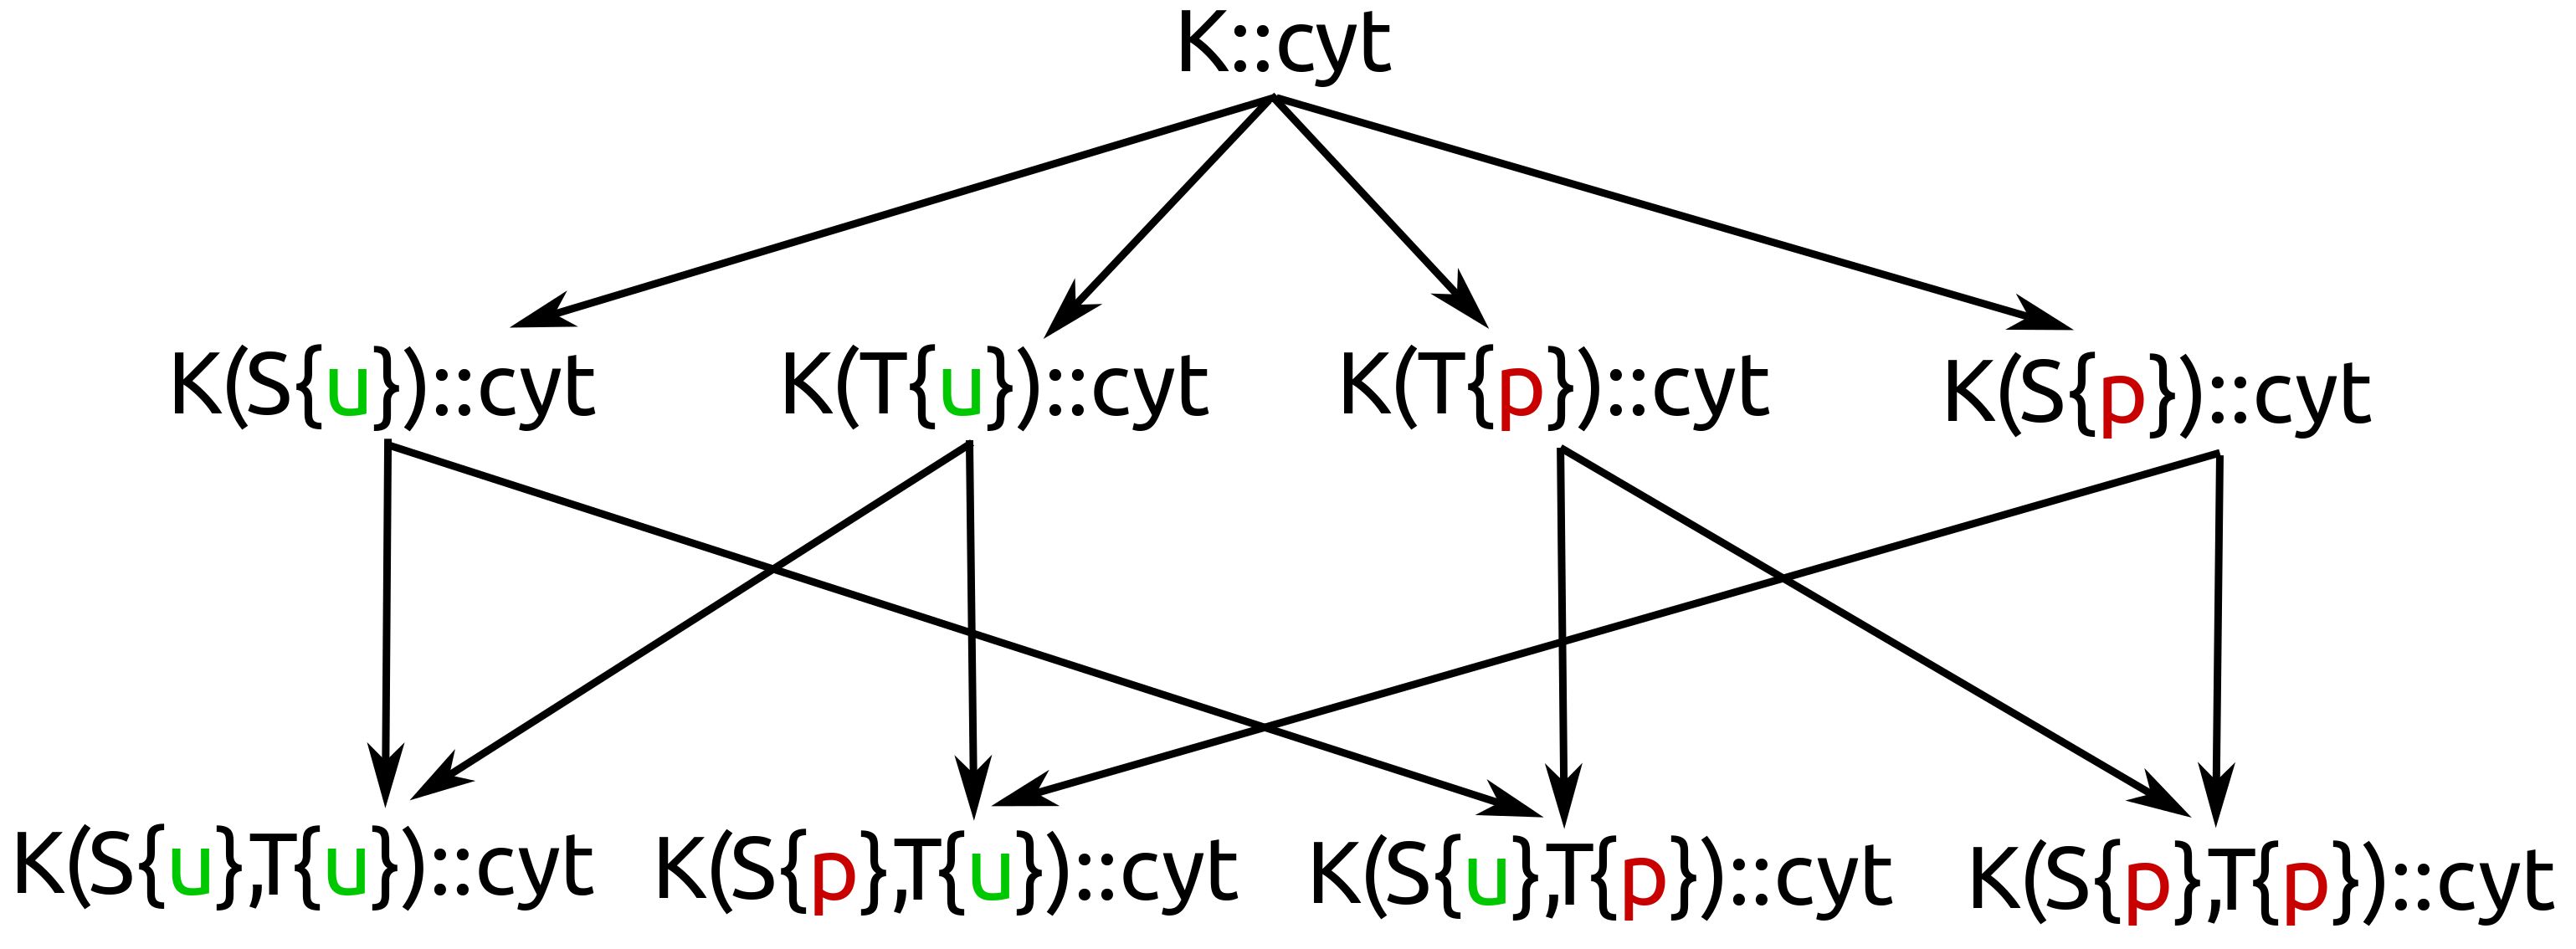
\includegraphics[scale=0.13]{pics/partial_order}
\end{center}
\caption{An example of compatible set $\mathscr{X}$. For better readability, the agents are written in BCSL syntax. The set is formed by a complex in $cyt$ compartment, which has only one structure agent $K$ in its sequence. The structure agent $K$ has allowed atomic agents $T$ and $S$ in its partial composition. These two atomic agents might occur in two states -- $u$ and $p$. The set is complete -- there are all relevant agents bounded by compatibility operator.}\label{compatible_set_example}
\end{figure}

\begin{lemma}
\label{exists_one_comp_set}
For every complex agent $\mathtt{X}$ there exists exactly one compatible set $\mathscr{X} \subseteq \mathds{X}$ such that $ \mathtt{X} \in \mathscr{X}$.
\end{lemma}

\begin{proof}
Let us assume a complex agent $\mathtt{X}$ belongs to two compatible sets, namely $\mathtt{X} \in \mathscr{X}_1, \mathscr{X}_2$. From the Definition~\ref{compatible_set} condition~(\ref{compatible_cond}) follows that there exists a $\mathtt{X}_1 \in \mathscr{X}_1$ such that $\mathtt{X} \lhd \mathtt{X}_1$. 

Then, the condition~(\ref{non_compatible_cond}) claims that no complex agent from $\mathscr{X}_1$ and no complex agent from $\mathscr{X}_2$ can be compatible. Namely, $\mathtt{X}_1 \in \mathscr{X}_1$ cannot be compatible with $\mathtt{X} \in \mathscr{X}_2$. However, $\mathtt{X}$ and $\mathtt{X}_1$ are compatible (namely $\mathtt{X} \lhd \mathtt{X}_1$). It follows $\mathtt{X} \not\in \mathscr{X}_2$, what is a contradiction. $\QEDA$

% via identity?
\end{proof}

Practically, compatible sets can be used for static analysis on level of complexes~\ref{context_reduction} and for finding non-trivial relationships between the rules~\ref{rule_redundancy}.

%\vspace*{0.5cm}\noindent\textbf{Note:} There always exists a compatible set $\mathscr{X}$ for a complex agent $\mathtt{X}$ which follows from Lemma~\ref{exists_one_comp_set}.

Note that there always exists a compatible set $\mathscr{X}$ for a complex agent $\mathtt{X}$ which follows from Lemma~\ref{exists_one_comp_set}.

\begin{definition}{Compatible subset}
\label{compatible_subset}
Let $\mathscr{X} \subseteq \mathds{X}$ be a compatible set and $\mathtt{X} \in \mathscr{X}$ a complex agent. A set $\mkern2mu\overline{\mkern-4.5mu \mathscr{X}} \subseteq \mathscr{X}$ is called \emph{compatible subset} of $\mathscr{X}$ w.r.t. $\mathtt{X}$ if the following holds:

\begin{center}
$ \mkern2mu\overline{\mkern-4.5mu \mathscr{X}} \subseteq \mathscr{X}: \forall \mathtt{X}' \in \mkern2mu\overline{\mkern-4.5mu \mathscr{X}}: (\mathtt{X}' \lhd \mathtt{X} \wedge \forall \mathtt{X}'' \in \mkern2mu\overline{\mkern-4.5mu \mathscr{X}}: \neg (\mathtt{X}'' \lhd \mathtt{X}') )$
\end{center}

where $\mathtt{X}' \neq \mathtt{X}''$.
\end{definition}


%\vspace*{0.5cm}\noindent\textbf{Note:} For any complex agent $\mathtt{X}$ there exists just one compatible subset. The reason follows from Lemma~\ref{exists_one_comp_set} and the definition of the subset.

Note that for any complex agent $\mathtt{X}$ there exists just one compatible subset. The reason follows from Lemma~\ref{exists_one_comp_set} and the definition of the subset (Definition~\ref{compatible_subset}).

\begin{remark}
\label{generating_vs_compatibility}
In the process of generating reactions from the rules (Section~\ref{Generating reactions}), we are using ground form function (Definition~\ref{ground_form}). The function basically adds context to individual complex agents (and its substructures). In the definition of the function we provided exact procedure how to generate such agents.

When we look at the process more theoretically, a set of appropriate complex agents is generated for every complex agent $\mathtt{X}$ in the rule $\mathtt{R}$ and then they are connected to multiple unique reactions. This set is actually a compatible subset $\mkern2mu\overline{\mkern-4.5mu \mathscr{X}}$ of compatible set $\mathscr{X}$ such that $\mathtt{X} \in \mathscr{X}$. In other words, agents of $\mkern2mu\overline{\mkern-4.5mu \mathscr{X}}$ are the minimal elements of set $\mathscr{X}$ w.r.t. compatibility with complex agent $\mathtt{X}$.

\end{remark}

\subsection{Rule redundancy elimination}
\label{rule_redundancy}

There might be cases when there are redundant rules defined in a model (Definition~\ref{redundant_rule}). This might be done for example by inattention of modeller in combination with high level of abstraction language uses. These rules do not cause any semantic difference, but can possibly slow down dynamic and/or static analysis, eventually undesirably affect the results of analysis.

\begin{definition}{Redundant rule expression}
\label{redundant_rule}

Let $\mathds{M}_1 = (\mathcal{R} \cup \{ \varrho \}, \Sigma_\mathtt{A}, \Sigma_\mathtt{T}, \mathtt{init})$ and
$\mathds{M}_2 = (\mathcal{R}, \Sigma_\mathtt{A}, \Sigma_\mathtt{T}, \mathtt{init})$ be BCSL models where $\varrho$ is a rule expression such that $\varrho \not\in \mathcal{R}$. We define the rule expression $\varrho$ as \emph{redundant} if $LTS(\mathds{M}_1) \equiv LTS(\mathds{M}_2)$.
\end{definition}

The redundant rule expression $\varrho$ does not add any semantic information to the model. It generally means the LTSs produced from the models with and without the rule expression are equal.

\begin{theorem}
\label{redundant_if}
Let $\varrho, \varrho'$ be two rule expressions of form:
\begin{center}
$ \Gamma_1 + \Gamma_2 + \ldots + \Gamma_n \Rightarrow \Gamma_{n+1} + \Gamma_{n+2} + \ldots + \Gamma_{m} $
\end{center}

for some $m,n \in \mathbb{N}$ such that $\mathtt{F}(\varrho), \mathtt{F}(\varrho')$ are well-formed rules. The rule expression $\varrho$ is \emph{redundant} if $ \forall i \in [ 1, m ]: \mathtt{F}(\Gamma_i) \lhd \mathtt{F}(\Gamma'_i). $
\end{theorem}

\begin{proof}
The problem whether the elimination of redundant rule expression preserves semantics can be reduced to a simple question -- if it holds for single pair of complex agents for a position $k$ in the appropriate rules, then it generally holds for entire rule, because the condition of redundancy holds for each pair of complexes independently.

The complex agents $\mathtt{X}_k = \mathtt{F}(\Gamma_k)$ and $\mathtt{X}'_k = \mathtt{F}(\Gamma'_k)$ both belong to the same compatible set $\mathscr{X}$ since $\mathtt{X}_k \lhd \mathtt{X}'_k$, which follows from the condition of the theorem. 

Then, we can create subsets $\mkern2mu\overline{\mkern-4.5mu \mathscr{X}},~ \mkern2mu\overline{\mkern-4.5mu \mathscr{X}'} \subseteq \mathscr{X}$ for both complex agents respectively (Definition~\ref{compatible_subset}). Because the complex agents are compatible ($\mathtt{X}_k \lhd \mathtt{X}'_k$ ), the subset $\mkern2mu\overline{\mkern-4.5mu \mathscr{X}}$ of agent $\mathtt{X}_k$ is either subset or equal to set $\mkern2mu\overline{\mkern-4.5mu \mathscr{X}'}$ of agent $\mathtt{X}'_k$:

$$\mkern2mu\overline{\mkern-4.5mu \mathscr{X}} \subseteq ~\mkern2mu\overline{\mkern-4.5mu \mathscr{X}'}.$$

Applied generally on entire rule, the produced set of reactions from the redundant rule is actually a subset of reactions produced from the non-redundant rule. $\QEDA$
\end{proof}

For the proof we used compatible sets of complex agents and the fact that when we are generating reactions from rules, we are actually enumerating all agents from the compatible set which are \emph{compatible with} original agent in the rule (Remark~\ref{generating_vs_compatibility}).

\begin{example}{Redundant rule expression}
Let us have two rule expressions:

\begin{enumerate}
	\item \label{rule_red_1} $K(S\{u\}).K::cell \Rightarrow K(S\{p\}).K::cell$
	\item \label{rule_red_2} $K(S\{u\}, T\{i\}).K::cell \Rightarrow K(S\{p\}, T\{i\}).K::cell$
\end{enumerate}

Considering structure signature $\Sigma_\mathtt{T}(K) = \{ S, T \} $ and atomic signatures $\Sigma_\mathtt{A}(S) = \{ u, p \} $ and $\Sigma_\mathtt{A}(T) = \{ a, i \} $, the rule expression (\ref{rule_red_1}) produces following set of eight reactions:

{\small
\begin{center}
$\Set{\begin{array}{l}
K(S\{u\}, T\{a\}).K(S\{u\}, T\{a\})::cell \Rightarrow K(S\{p\}, T\{a\}).K(S\{u\}, T\{a\})::cell,\\
K(S\{u\}, T\{a\}).K(S\{u\}, T\{i\})::cell \Rightarrow K(S\{p\}, T\{a\}).K(S\{u\}, T\{i\})::cell,\\
K(S\{u\}, T\{a\}).K(S\{p\}, T\{a\})::cell \Rightarrow K(S\{p\}, T\{a\}).K(S\{p\}, T\{a\})::cell,\\
K(S\{u\}, T\{a\}).K(S\{p\}, T\{i\})::cell \Rightarrow K(S\{p\}, T\{a\}).K(S\{p\}, T\{i\})::cell,\\
K(S\{u\}, T\{i\}).K(S\{u\}, T\{a\})::cell \Rightarrow K(S\{p\}, T\{i\}).K(S\{u\}, T\{a\})::cell,\\
K(S\{u\}, T\{i\}).K(S\{u\}, T\{i\})::cell \Rightarrow K(S\{p\}, T\{i\}).K(S\{u\}, T\{i\})::cell,\\
K(S\{u\}, T\{i\}).K(S\{p\}, T\{a\})::cell \Rightarrow K(S\{p\}, T\{i\}).K(S\{p\}, T\{a\})::cell,\\
K(S\{u\}, T\{i\}).K(S\{p\}, T\{i\})::cell \Rightarrow K(S\{p\}, T\{i\}).K(S\{p\}, T\{i\})::cell \end{array}}$
\end{center}
}

while the rule expression (\ref{rule_red_2}) produces set of reaction which a subset of the previous one:

{\small
\begin{center}
$\Set{\begin{array}{l}
K(S\{u\}, T\{i\}).K(S\{u\}, T\{a\})::cell \Rightarrow K(S\{p\}, T\{i\}).K(S\{u\}, T\{a\})::cell,\\
K(S\{u\}, T\{i\}).K(S\{u\}, T\{i\})::cell \Rightarrow K(S\{p\}, T\{i\}).K(S\{u\}, T\{i\})::cell,\\
K(S\{u\}, T\{i\}).K(S\{p\}, T\{a\})::cell \Rightarrow K(S\{p\}, T\{i\}).K(S\{p\}, T\{a\})::cell,\\
K(S\{u\}, T\{i\}).K(S\{p\}, T\{i\})::cell \Rightarrow K(S\{p\}, T\{i\}).K(S\{p\}, T\{i\})::cell \end{array}}$
\end{center}
}

\end{example}

\subsection{Context-based reduction}
\label{context_reduction}

There might be cases when eliminating context of the given BCSL model preserves some properties while making the analysis of the model simpler. This is particularly case of dynamic analysis, where minor change in the model specification can dramatically affect the behaviour. To make it possible, we have to define such a reduced model and show what kind of information does it preserve.

\begin{definition}{Reduced model}
\label{reduced_model}
Let $\mathds{M} = (\mathcal{R}, \Sigma_\mathtt{A}, \Sigma_\mathtt{T}, \mathtt{init})$ be a BCSL model. We define \emph{reduced model} $\widetilde{\mathds{M}}$ as a pair $(\widetilde{\mathcal{R}}, \mathtt{I})$ where $\widetilde{\mathcal{R}}$ is set of rule expression and $\mathtt{I}$ is initial multiset of complex agent expressions where the following conditions hold:

\begin{enumerate}
	\item for every well-formed rule $\mathtt{F}(\varrho') = (\chi', \omega', \iota', \varphi', \psi') \in \mathds{R}$ such that $\varrho' \in \widetilde{\mathcal{R}}$ and appropriate original rule $\mathtt{F}(\varrho) = (\chi, \omega, \iota, \varphi, \psi) \in \mathds{R}$ such that $\varrho \in \mathcal{R}$ holds:

	\begin{center}
	$\forall i \in [1, k]: \pi_i(\chi') \equiv \mathtt{sup}(\mathscr{X})$
	\end{center}

	where $\mathscr{X}$ is a compatible set such that $\pi_i(\chi) \in \mathscr{X}$, length $k = |\chi'| = |\chi|$ (i.e., the number of complex agents in both rules is the same), and $\iota = \iota'$;

	\item for every complex agent $\mathtt{X}' = \mathtt{F}(\Gamma') \in \mathtt{I}$ and appropriate original complex agent $\mathtt{X} = \mathtt{F}(\Gamma) \in \mathtt{init}$ the following condition holds:

	\begin{center}
	$ \mathtt{X}' \equiv \mathtt{sup}(\mathscr{X}) $ such that $\mathtt{X} \in \mathscr{X}$.
	\end{center}
\end{enumerate}
\end{definition}

Reduced model $\widetilde{\mathds{M}}$ is created form given BCSL model by reducing context of complexes in rules to maximum level. This is achieved by taking supremum from compatible set $\mathscr{X}$. This procedure might produce rules with no action, i.e. not well-formed rules -- such rules are omitted. Then, only rules creating/destroying agents and complex formation/dissociation should remain, providing reduced network. Since we are reducing context, the resulting network can be equal or smaller than the original one.

\begin{definition}{Compatibility of states}
Let $\mathds{M}$ be a BCSL model and $\mathtt{s}_1, \mathtt{s}_2 \in S$ of $LTS(\mathds{M})$ two states from its LTS. The state $\mathtt{s}_1$ is \emph{compatible with} state $\mathtt{s}_2$, written $\mathtt{s}_1 \lhd \mathtt{s}_2$, \emph{iff} 

\begin{center}
$\forall \mathtt{X}_1 \in \mathtt{s}_1 \exists \mathtt{X}_2 \in \mathtt{s}_2: \mathtt{sup}(\mathscr{X}) \equiv \mathtt{X}_2 $
\end{center}

such that $\mathscr{X} \subseteq \mathds{X}$ is a compatible set and $\mathtt{X}_1 \in \mathscr{X}$.

\end{definition}

\begin{definition}{Over-approximation of LTS}
\label{over_approximation}

Let $LTS, LTS'$ be labelled transition systems of some BCSL models. The $LTS'$ is \emph{over-approximation} of $LTS$ if for every path $\mathtt{s}_1' \mathtt{s}_2' \mathtt{s}_3' \ldots \mathtt{s}_n'$ in $LTS'$ there exists a path $\mathtt{s}_1 \mathtt{s}_2 \mathtt{s}_3 \ldots \mathtt{s}_m$ in LTS such that:

\begin{center}
$\forall \mathtt{s}'_i, \mathtt{s}'_{i+1} \exists \mathtt{s}_k, \mathtt{s}_l : l > k \wedge \mathtt{s}_k \lhd \mathtt{s}'_i \wedge \mathtt{s}_l \lhd \mathtt{s}'_{i+1} $.
\end{center}

\end{definition}

A reduced model $\widetilde{\mathds{M}}$ is actually an over-approximation of a BCSL model $\mathds{M}$ in context of their LTSs (Definition~\ref{over_approximation}). It can be used for some types of analyses which avoid combinatorial explosion of the original model $\mathds{M}$.

\begin{theorem}
\label{non-reachability_in_reduced}
Let $\mathtt{X}$ be a complex agent, $\mathscr{X}$ be a compatible set for $\mathtt{X}$, $\mathds{M}$ be a given BCSL model, and $\widetilde{\mathds{M}}$ be an appropriate reduced model of model $\mathds{M}$. If supremum $\mathtt{sup}(\mathscr{X})$ is non-reachable in $LTS(\widetilde{\mathds{M}})$, then agent $\mathtt{X}$ is also non-reachable in the $LTS(\mathds{M})$.
\end{theorem}

\begin{proof}
Let us assume a complex agent $\mathtt{sup}(\mathscr{X})$ is non-reachable in $LTS(\widetilde{\mathds{M}})$, but $\mathtt{X} \in \mathscr{X}$ is reachable in $LTS(\mathds{M})$.

Generally, there is a path formed from rules in the $LTS(\mathds{M})$ such that we transform complex agents from initial agents to desired complex agent $\mathtt{X}$. When we move to context of $LTS(\widetilde{\mathds{M}})$, there is no such path for $\mathtt{sup}(\mathscr{X})$. According to Definition~\ref{reduced_model}, for every such rule there exists a reduced rule, such that all interacting complexes are reduced to their supremas. Therefore, if we could apply an original rule on a complex agent, we can do the same with reduced rule and its supremum. It follows there must exist such path also in $LTS(\widetilde{\mathds{M}})$ and the complex agent $\mathtt{sup}(\mathscr{X})$ is reachable, what is a contradiction. $\QEDA$
\end{proof}

If we are checking whether an agent is reachable in $LTS(\mathds{M})$ for given model $\mathds{M}$, we might first check whether its super-ancestor is reachable in $LTS(\widetilde{\mathds{M}})$ of appropriate reduced model $\widetilde{\mathds{M}}$. If it holds, then we are still not certain about reachability of agent itself and it has to be checked in the $LTS(\mathds{M})$. However, agent which is not reachable in $LTS(\widetilde{\mathds{M}})$ is also not reachable in $LTS(\mathds{M})$ (Theorem~\ref{non-reachability_in_reduced}).

\subsection{Static reachability analysis}
\label{static_reachability_analysis}

Since we have defined compatibility operator for agents, we can apply static reachability analysis before enumerating whole state space of the model $\mathds{M}$. This analysis has its limitations, but can serve for checking whether a complex agent $\mathtt{X}$ is \emph{non-reachable} (similar to Section~\ref{context_reduction}).

\begin{theorem}
\label{static_reach}
Let $\mathcal{R}_f$ be a set of rules created from set of rule expressions $\mathcal{R}$ of given model $\mathds{M}$ using semantic function $\mathtt{F}$ and $\mathtt{X}$ be a complex agent. The complex agent $\mathtt{X}$ is non-reachable w.r.t. set of rules $\mathcal{R}_f$ \emph{if}:

\begin{center}
$\forall~ \mathtt{R} \in \mathcal{R}_f: \forall i \in [\iota+1, \ldots, |\chi|] : \neg ( \pi_i(\chi) \lhd \mathtt{X})$
\end{center}

\noindent such that $\mathtt{R} = (\chi, \omega, \iota, \varphi, \psi)$.
\end{theorem}

\begin{proof}
Let us assume we have a path of states constructed by applying corresponding reactions created from rules $\mathcal{R}_f$ where $\mathtt{X}$ is reachable. At some point on the path, we inevitably have to create a complex agent $\mathtt{X}_2 \lhd \mathtt{X}$ from a complex agent $\mathtt{X}_1$ applying a rule $\mathtt{R}$. 

\begin{center}

\includegraphics[scale=0.15]{pics/static_reach}
\end{center}

It requires there has to be a complex agent $\mathtt{X}_2'$ in the rule which is compatible with the complex agent $\mathtt{X}_2$. If there is not such an agent, the agent $\mathtt{X}$ is non-reachable. $\QEDA$
\end{proof}

The Theorem~\ref{static_reach} states a very powerful fact in context of non-reachability analysis. Compared to dynamic non-reachability analysis, it completely avoids any combinatorial explosion and gives answer only by testing structural properties of rules.

This procedure can be extended for checking reachability of multiple complex agents. However, it does not consider stoichiometry.

\subsection{Automatic synthesis of signatures}

The BCSL model definition as given in Section~\ref{BCSl_model} can be reduced by signatures. Note we do not mean extended signatures by complex names (Section~\ref{complex_signature}) -- just the basic signatures for atomic and structure agents. These can be obtained statically from the rules (and the initial state) in a  linear process. The process comprises these steps:

\begin{enumerate}
\item prepare empty signature sets $\Sigma_\mathtt{A}$ and $\Sigma_\mathtt{T}$, 
\item create rule $\mathtt{R} = (\chi, \omega, \iota, \varphi, \psi)$ for every rule expression $\varrho$ using semantic function $\mathtt{F}$,
\item iterate through all $\omega \in \mathtt{R}$ and:
\begin{enumerate}
  \item \label{atomic_iter} for every atomic agent $\mathtt{A}$ do the following:
  	\begin{enumerate}
  		\item \textbf{if} $\exists x \in \Sigma_\mathtt{A}: \eta(\mathtt{A}) \equiv \pi_1(x) $ 

  		\textbf{then} $\delta(\mathtt{A}) \mapsto \pi_2(y)$

  		\textbf{else} $(\eta(\mathtt{A}), \{~\delta(\mathtt{A})~\}) \mapsto \Sigma_\mathtt{A}$;
	\end{enumerate}
  \item \label{structure_iter} for every structure agent $\mathtt{T}$ do the following:
	\begin{enumerate}
	  \item \textbf{if} $\exists x \in \Sigma_\mathtt{T}: \eta(\mathtt{T}) \equiv \pi_1(x) $

	  \textbf{then} $\forall \mathtt{A} \in \gamma(\mathtt{T}): \eta(\mathtt{A}) \mapsto \pi_2(y)$ and 

	  \hspace*{1cm} do step~\ref{atomic_iter} with every atomic agent $\mathtt{A}$

	  \textbf{else} $(\eta(\mathtt{T}), \{ \eta(\mathtt{A}) ~|~ \mathtt{A} \in \gamma(\mathtt{T}) \}) \mapsto \Sigma_\mathtt{T}$ 

	  \hspace*{0.75cm} do step~\ref{atomic_iter} with every atomic agent $\mathtt{A}$.
	\end{enumerate}
\end{enumerate}
\end{enumerate}

The described process basically iterates through all rules and collects all atomic names and states associated with them. Similarly, it collects all structure names and appropriate names of atomic agents used in their partial compositions. In this case, atomic information has to be collected recursively because some atomic agents might be used only in partial composition, not independently in a complex.

We can discuss the fact that desired signature might be in some manner \emph{larger} than the collected one. However, if for example we want to have more states defined for an atomic agent, they should be definitely used somewhere in the model. In other case, it does not play any role in the model behaviour and therefore its definition is senseless. In other words, the described procedure guarantees collecting all signature details which play any role in the model.

% \begin{proof}
% Let $\mathcal{M}$ be a BCSL model and $\Sigma$ its minimal signatures (i.e., all states and partial compositions defined in the signatures are actually used in the rules). Then, signatures $\Sigma'$ obtained by procedure (ref blah) has to be equal to the original signature $\Sigma$. In case its not, it means either there is some extra data in the $\Sigma'$ or some data is missing. Since we create $\Sigma'$ by iterating through all the rules, we construct complete signature with complete states used in the model. Therefore, if some data are missing in $\Sigma'$, then it follows given signature $\Sigma$ is not minimal. On the other hand, if there are some extra data in $\Sigma'$, then given signature $\Sigma$ is incorrect -- its missing some structure details which are being used in the model. $\QEDA$
% \end{proof}

\subsection{Translation to Petri Net}

By generating reaction-based model from rule-based, which is always possible (Section~\ref{Generating reactions}), we can furthermore translate such model to a Petri Net~\cite{petri}.

The translation can be summarised in the following steps: 

\begin{enumerate}
\item since BCSL rules produce a finite number of reactions, we have also a finite number of unique agents -- these are the places \emph{P},
\item the transitions \emph{T} are the reactions,
\item set of arcs $F$ is created from all reactions as following:
\begin{itemize}
  \item place input arc from each place which has label in left-hand side of the reaction (with appropriate multiplicity),
  \item do the same for output arcs for right-hand side of the reaction,
\end{itemize}
\item create initial marking \emph{m} from given initial state of the model by similar procedure described above.
\end{enumerate}

Once the model is translated, we are allowed to apply all available types of analyses which are provided by Petri Nets. For example, P and T invariants, deadlock detection, coverability etc. (more details in \cite{petri}).

\subsection{Minimal optimal bound of the system}
\label{optimal_bound}

Transition systems produced by semantics of BCSL models are infinite in general. Despite the fact the underlying reaction networks are always finite (Section~\ref{optimal_bound}), there are types of reactions which can increase number of occurrences in a state with no limitations. Typically, such reactions form an interface between the modelled system and the environment.

However, the process of applying vector reactions on states can be extended by a control system. This system does not allow to grow individual values inside the state vector above given \emph{bound} $\mathtt{B}$. Basically, if produced vector should obtain an integer higher than the bound, the action is not taken. This procedure is very similar to checking whether all values in the vector are positive. Instead of only lower bound, we have two bounds $<0, \mathtt{B}>$.

The remaining issue is what is an optimal value for the bound. The universal solution is to let the modeller decide. It follows extension of model definition by the bound. However, this process requires the user to know additional information about the model and additional effort. It does not fit to purposes of the language.

Therefore we decided to apply a static analysis on the model. We will not provide a formal definition of this analysis, rather give intuition and reason about this particular solution.

We decided to find a minimal bound, which is in this context optimal for generating all required objects. It means that all the complexes which are potentially encoded in rules  will be produced in at least one repetition. In other words, with this bound a minimal network should be created. In such network, every agent reachable in boundless network is reachable also in minimal network (which does not hold when we take stoichiometry into the account).

To actually calculate the minimal bound we take maximum value from the following measurements:

\begin{enumerate}
  \item \label{count_init} count the highest number of occurrences from all complex agents in initial state,
  \item \label{count_unique} count the highest number of unique atomic and structure agents in every complex agent of all rules,
  \item \label{count_stoi} count the highest stoichiometry in every left and right-hand side of the rules.
\end{enumerate}

The step~(\ref{count_init}) ensures the bound $\mathtt{B}$ will not be lower than highest number of equivalent agents in the initial state. In the step~(\ref{count_unique}) we count repetitions of equivalent atomic and structure agents inside all complexes, which ensures that there will be enough agents for creation of every complex agent. The last step~(\ref{count_stoi}) takes into the account stoichiometry used in context of complex agents themselves.

This should guarantee that it is possible to achieve high enough number of occurrences to produce any complex or combination of complexes.

\chapter{Case study}
\label{case_study}

%To demonstrate Biochemical Space has practical use, we introduce an instance of CMP, where it is used in practice.
E-cyanobacterium.org~\cite{Trojak2016} is an online platform providing tools for public sharing, annotation, analysis, and visualization of dynamical models and wet-lab experiments related to cyanobacteria. The general aim is to stimulate collaboration between experimental and computational systems biologists to achieve better understanding of cyanobacteria. As an instance of CMP, it covers all the features of the platform.

The following processes of cyanobacteria are covered in BCS: environmental processes, respiration and photosynthesis, carbon concentrating mechanism, circadian clock, and metabolism. Currently, the repository of models contains two models describing circadian clock (Miyoshi et al. 2007~\cite{Miyoshi01022007}, Hertel et al. 2013~\cite{Hertel2013}) and a kinetic model of metabolism (Jablonsky et al. 2014~\cite{Jablonsky2014}). Two other models present unpublished results -- dynamics of carbon fluxes (M\"{u}ller et al.) and photosynthesis (Plyusnina et al.). Additionally, two models in development describing carbon concentrating mechanism are Clark et al. 2014~\cite{clark2014insights} and Fridlyand et al. 1995~\cite{fridlyand1996quantitative}. Each of them was properly mapped on the BCS and helped to form suitable space covering all the mentioned processes.

Entire biochemical space of cyanobacteria is formed from over 1000 entities and 600 rules. Therefore, we will not explain all of them here, we provide a several cases which demonstrate how different BCSL features can be used for describing particular biological problems.

The circadian clock of cyanobacteria~\cite{CCR} is formed by three proteins $KaiA$, $KaiB$, and $KaiC$ (with additional presence of $ATP$). The key role plays $KaiC$. Compared to the other two proteins, it is physically the largest one. Its primary structure is a sequence of amino acids, where two particular are important for the modelling -- threonine 432 and serine 431. These two amino acids can be enriched by phosphoryl group in process commonly known as phosphorylation~\cite{cohen2002origins}. However, the sites are accessible only when the protein forms a homohexamer -- a structure of six $KaiC$ proteins. For the phosphorylation $KaiA$ proteins are responsible while $KaiB$ proteins inactivate $KaiA$s, which leads to autodephosphorylation of $KaiC$ protein. There are several complexes which can be formed from mentioned proteins according to current situation with the $KaiC$ hexamer (Figure~\ref{phospho_rule}).

It is important to note the $KaiA$ and $KaiB$ proteins only \emph{enhance} (resp. \emph{suppress}) the phosphorylation process, but do not enable/disable it completely. When it comes to quantitative description of the system, it is necessary to depict all possible actions. Particularly, we need to express the fact the phosphorylation process happens regardless the particular complex $KaiC$ protein is currently in. 

\begin{figure}[!h]
{\small
\begin{center}
$ S\{u\}::KaiC::~?X::cyt \Leftrightarrow S\{p\}::KaiC::~?X::cyt ~;~$

$ ?X = \{~KaiC6, KaiA2C6, KaiA4C6, KaiB6C6, KaiA4B6C6, KaiA6B6C6~\} $
\end{center}
}
\caption{Phosphorylation rule of serine residue for all possible of complexes with $KaiC$ included. A variable $?X$ is used in place of all possible complexes. Notice there is also a $KaiC6$ complex, which corresponds to auto-(de)phosphorylation.}\label{phospho_rule}
\end{figure}

Another interesting aspect of the cyanobacterial circadian clock mechanism is formation of $KaiC$ hexamers. The condition that the $KaiC$ protein can be (de)phosphorylated \emph{only} inside a hexamer leads to one important fact -- it does not mean the hexamer must be assembled from (resp. dissociated to) unphosphorylated $KaiC$ proteins. The hexamer can be dissociated at any point in time, for example when three $KaiC$s are phosphorylated on the serine residue, other two are phosphorylated on both residues, and the last one is not phosphorylated. The number of possible combinations is quite huge.

Rule-based languages including BCSL are very suitable for such cases. What we actually need to express is situation, when a complex is formed (or dissolved) regardless the context (particular states) of the interacting entities (Figure~\ref{hexamer_rule}).

\begin{figure}[!h]
{\small
\begin{center}
$ 6 ~KaiC::cyt \Leftrightarrow KaiC6::cyt $
\end{center}
}
\caption{Formation of KaiC hexamer from six KaiC proteins and its dissociation. The rule requires to have a defined complex name $KaiC6$ in the corresponding BCS.}\label{hexamer_rule}
\end{figure}

Another important process inside cyanobacteria is photosynthesis. It is performed on internal membranes called thylakoids. In general, photosynthesis in cyanobacteria uses water as an electron donor and produces oxygen as a product. Electron transport is performed though multiple protein complexes, which together form the thylakoid membrane itself. Such complexes are for example photosystem I and II (Figure~\ref{ps2_rule}). However, direct modelling of the complexes is not very efficient. The typical rules in photosynthesis are just electron transfers between the complexes or reduction/oxidation of individual parts. Therefore, such action usually happen regardless the context of the rest of the complexes in a photosystem. The best approach with respect to BCSL language is to use structure agent for defining the protein complexes and its individual parts model as partial composition.

\begin{figure}[!h]
{\small
\begin{center}
$ ps2(oec\{2+\}, yz\{+\})::tlm \Leftrightarrow ps2(oec\{3+\}, yz\{n\})::tlm $
\end{center}
}
\caption{Oxidation of S2-state of the oxygen-evolving complex $oec{2+}$ by $Yz{+}$ in photosystem II. There are many more subparts of photosystem II. (e.g. chlorophyl, pheophytin), but their states are not important in this case.}\label{ps2_rule}
\end{figure}

We want to demonstrate practical purposes of a few types of static analyses defined in Section~\ref{static_analyses}. Yamada et al. 2004~\cite{yamada2004model} is a model of \emph{fibroblast growth factor} (FGF) signalling pathway. The model represents a signalling pathway, which is typically a cascade of signal transduction. It means if something goes wrong on a particular point in the cascade, it will influence the rest of the pathway. Entire model written in BCSL syntax is provided in Appendix~\ref{yamada_complete}. It consists of 20 entities interacting in 56 rules. Most of proteins can undergo phosphorylation (state change from $u$ to $p$ on some amino acid residues). We consider initial conditions such that there are all required entities in one or two repetitions (some complexes require multiplicity). In such case, the number of reachable state grows up to $2^{72}$, which too high to be effectively enumerated.

In Figure~\ref{fgf_fragment}, there is the model defined in BCSL syntax. Note this model is a fragment of the entire model. Focus on the rule~(\ref{focus_rule}). It requires both Threonine residues ($Thr$) on $FGF$ proteins to be phosphorylated ($p$). Basically, it is not possible to create a complex from $FRS$ and unphosphorylated ($u$) $FGF$ proteins.

For example, we want to check whether a given complex agent {\small $FRS(Thr\{u\}, Tyr\{u\}).FGF(Thr\{u\}).R.FGF(Thr\{u\}).R::cyt$} is reachable for the given model. The agent is formed from $FGF$ proteins which are unphosphorylated ($u$) on threonine residues ($Thr$). In traditional approach, we have to enumerate entire state space of the model and then use dynamic model checking method to check it. In our case, we can use Theorem~\ref{static_reach} and check if it is non-reachable using static reachability analysis. It results to conclusion that there is no compatible agent on any right-hand side of the rules. It follows the complex agent is non-reachable.

\begin{figure}[!h]
{\footnotesize
\begin{center}
\begin{enumerate}
\item $FGF::cyt + R::cyt \Leftrightarrow FGF.R::cyt$ 
\item $2~ FGF.R::cyt \Leftrightarrow FGF.R.FGF.R::cyt$
\item $FGF(Thr\{u\}).R.FGF.R::cyt \Leftrightarrow FGF(Thr\{p\}).R.FGF.R::cyt$ 
\item \label{focus_rule} $FRS(Thr\{u\})::cyt + FGF(Thr\{p\}).R.FGF(Thr\{p\}).R::cyt \Rightarrow$ 

$\Rightarrow FRS(Thr\{u\}).FGF(Thr\{p\}).R.FGF(Thr\{p\}).R::cyt$ 

\item $FRS(Thr\{u\}).FGF.R.FGF.R::cyt \Rightarrow FRS(Thr\{p\}).FGF.R.FGF.R::cyt$ 

\end{enumerate}

$\vdots$

\vspace*{0.5cm}
Initial conditions:
\begin{tabular}{l}
$2~ FGF(Thr\{u\})::cyt$\\
$2~ R::cyt$\\
$1~ FRS(Thr\{u\}, Tyr\{u\})::cyt$\\
\end{tabular}

$\vdots$

\end{center}

}
\caption{A fragment of the model Yamada et al. 2004~\cite{yamada2004model} of FGF signalling pathway written in BCSL. The complete model can find in Appendix~\ref{yamada_complete}.}\label{fgf_fragment}
\end{figure}

Demonstration of context-based reduction (Section~\ref{context_reduction}) is provided on the same model as in the previous case. Now we can compute with entire model since we will reduce its context to minimum. In Figure~\ref{reduced_yamada} there are 16 bidirectional rules which we have created by applying Definition~\ref{reduced_model}. The size of state space has significantly decreased -- it has 606 states and 2015 edges.

For the analysis itself, we could for example ask about reachability of a complex agent {\small $Raf(Thr\{p\}).ERK(Tyr\{p\},Thr\{p\})::cyt$} in the original model (Appendix~\ref{yamada_complete}). We can first check whether its supremum (from the corresponding compatible set $\mathscr{X}$) {\small $Raf.ERK::cyt$} is non-reachable in the reduced model. Since the state space of the model is relatively small, it is not a problem using dynamical model checking. Using the Theorem~\ref{non-reachability_in_reduced}, the answer is non-reachable.

\begin{figure}[!h]
\begin{center}
{\small
\begin{tabular}{r c l}
$FGF::cyt + R::cyt $ & $ \Leftrightarrow $ & $ FGF.R::cyt$\\
$FGF.R::cyt + FGF.R::cyt $ & $ \Leftrightarrow $ & $ FGF.R.FGF.R::cyt$\\
$FRS::cyt + FGF.R.FGF.R::cyt $ & $ \Leftrightarrow $ & $ FGF.R.FGF.R.FRS::cyt$\\
$FRS::cyt + SHP::cyt $ & $ \Leftrightarrow $ & $ FRS.SHP::cyt$\\
$GS::cyt + GPP::cyt $ & $ \Leftrightarrow $ & $ GS.GPP::cyt$\\
$GS::cyt + ERK::cyt $ & $ \Leftrightarrow $ & $ GS.ERK::cyt$\\
$FRS::cyt + GS::cyt $ & $ \Leftrightarrow $ & $ FRS.GS::cyt$\\
$Ras::cyt + FRS.GS::cyt $ & $ \Leftrightarrow $ & $ FRS.GS.Ras::cyt$\\
$Ras::cyt + GAP::cyt $ & $ \Leftrightarrow $ & $ GAP.Ras::cyt$\\
$Raf::cyt + Ras::cyt $ & $ \Leftrightarrow $ & $ Ras.Raf::cyt$\\
$Raf::cyt + PP::cyt $ & $ \Leftrightarrow $ & $ PP.Raf::cyt$\\
$MEK::cyt + Raf::cyt $ & $ \Leftrightarrow $ & $ Raf.MEK::cyt$\\
$MEK::cyt + XPP::cyt $ & $ \Leftrightarrow $ & $ XPP.MEK::cyt$\\
$ERK::cyt + MEK::cyt $ & $ \Leftrightarrow $ & $ MEK.ERK::cyt$\\
$ERK::cyt + MKP::cyt $ & $ \Leftrightarrow $ & $ MKP.ERK::cyt$\\
$ERK::cyt + FRS::cyt $ & $ \Leftrightarrow $ & $ ERK.FRS::cyt$\\
\end{tabular}
}
\end{center}
\caption{Model Yamada et al. 2004~\cite{yamada2004model} with reduced context according to Definition~\ref{reduced_model}.}\label{reduced_yamada}
\end{figure}

\chapter{Implementation}
\label{implementation}

In order to support usability of the BCSL language, we developed a prototype software tool BCSgen. The general goal of the tool is to provide environment suitable for editing and maintenance of the BCSL models and provide functionality to analyse the models. The software was developed in several iterations. At first as a project MUNI33/092015 in \emph{Dean's Program of the Faculty of Informatics MU for support of student research and development projects}, later as part of the project MUNI33/062017 in the same program. It was finalized to current stage in this thesis.

The tool is developed in Python language (version 2.7) as open-source desktop software build under GPL-3.0 license. The source code, a short tutorial for usage and installation, and current stable version as binary files are available on GitHub\footnotemark[1]\footnotetext[1]{\url{https://github.com/sybila/BCSgen}}.

In the first version, there was no support for editing the models. The only functionality provided by the tool was import of the model from a text file (in a predefined format) and enumerating entire state space of the model. The implementation was done by translating to Kappa and it was rather slow and non-efficient. The single transaction (application of one rule) was delayed by translation to Kappa and then by exact matching and replacement, which might get quite complicated. However, it was a good start for the language and it was possible to analyse exported networks in external tools. There was simple GUI made in Tkinter~\cite{Tkinter}, which had several issues. The most important one was the fact that Tkinter was not designed for multithreading programming. For example, while computing a state space for the model, the whole GUI was not responsible.

In the second version, we focused on speed improvement and development of a user-friendly GUI. For the speed improvement, we implemented semantics as defined in this thesis (Section~\ref{semantic_function}). Compared to previous version, in this case there was no exactly rule-based execution of the rule -- we rather translated the rules to the reactions and subsequently encoded as vector operations over integers. Therefore, one transaction was just addition of one vector (left-hand side) and subtraction of another one (right-hand side). The GUI was reimplemented in PyQt4~\cite{summerfield2007rapid}, which naturally works with multithreading. It was significant improvement from performance point of the view. Moreover, we improved input/output formats. For input we defined BCSL model format, which serves for import. As output format we have chosen JSON~\cite{json}, which is very suitable for its simplicity and support by many external tools.

\begin{figure}[!h]
\begin{center}
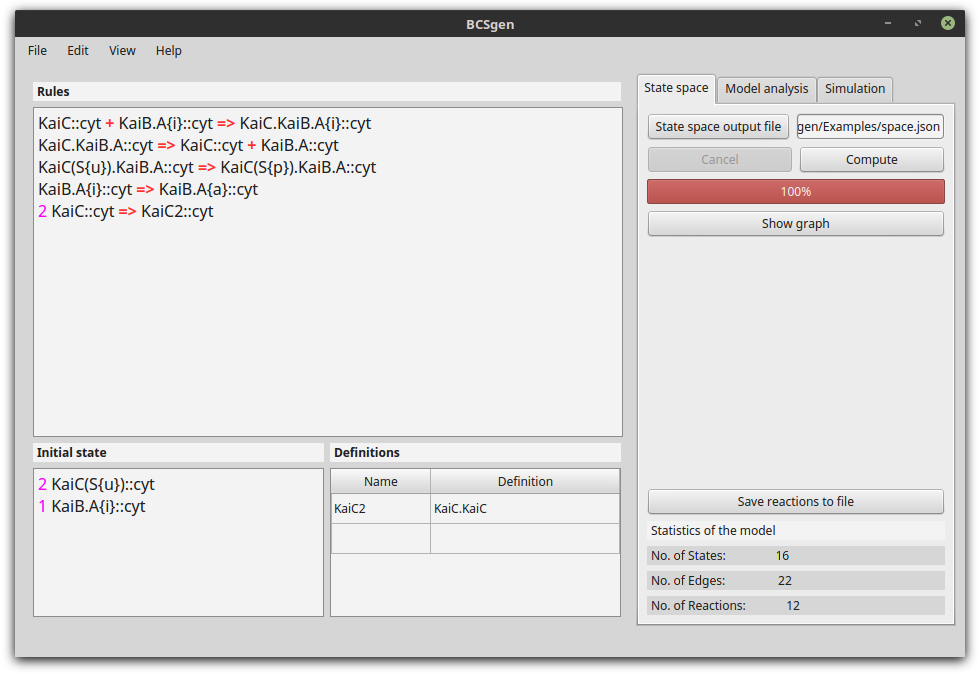
\includegraphics[scale=0.35]{pics/BCSgen_gui}
\caption{A screenshot of Graphical User Interface of BCSgen tool. There are a field for editing rules with integrated rule parser, field for initial state, and a table for defining custom names for complexes. On the right, there are options to analyse the model and display visualisations.}\label{gui_example}
\end{center}
\end{figure}

In the last version, which is part of this thesis, we focused on improvement of models maintenance, additional analysis services, and visualisation. We have integrated editor which is able to highlight syntax errors while building the model (Figure~\ref{gui_example}). To achieve this, we needed an efficient rule-parser which would be able to parse the rules very fast. The parser is able to parse even syntactic extensions defined in Section~\ref{syntactic_extensions}. The rules engine then translates the rule to ground form and creates reactions (in case there are no errors in the model). Since this engine runs in the background, user does not notice any increased performance. When reactions are computed, it is indicated by possibility to export them and generate state space of the model.

We implemented some dynamic analysis -- model simulation and reachability analysis. For the simulation, we allow stochastic or deterministic form (Figure~\ref{gui_simulation}). In the first form, random rules are fired according to Poisson distribution while in latter average trace is computed by solving ODEs build from the reactions. For the stochastic case, there are options to choose number of runs and apply interpolation on resulting time series chart in order to achieve smoother results. It is important to note that only models with defined rates can be simulated. For simplicity, approach where only fully specified agents are used.

\begin{figure}[!h]
\begin{center}
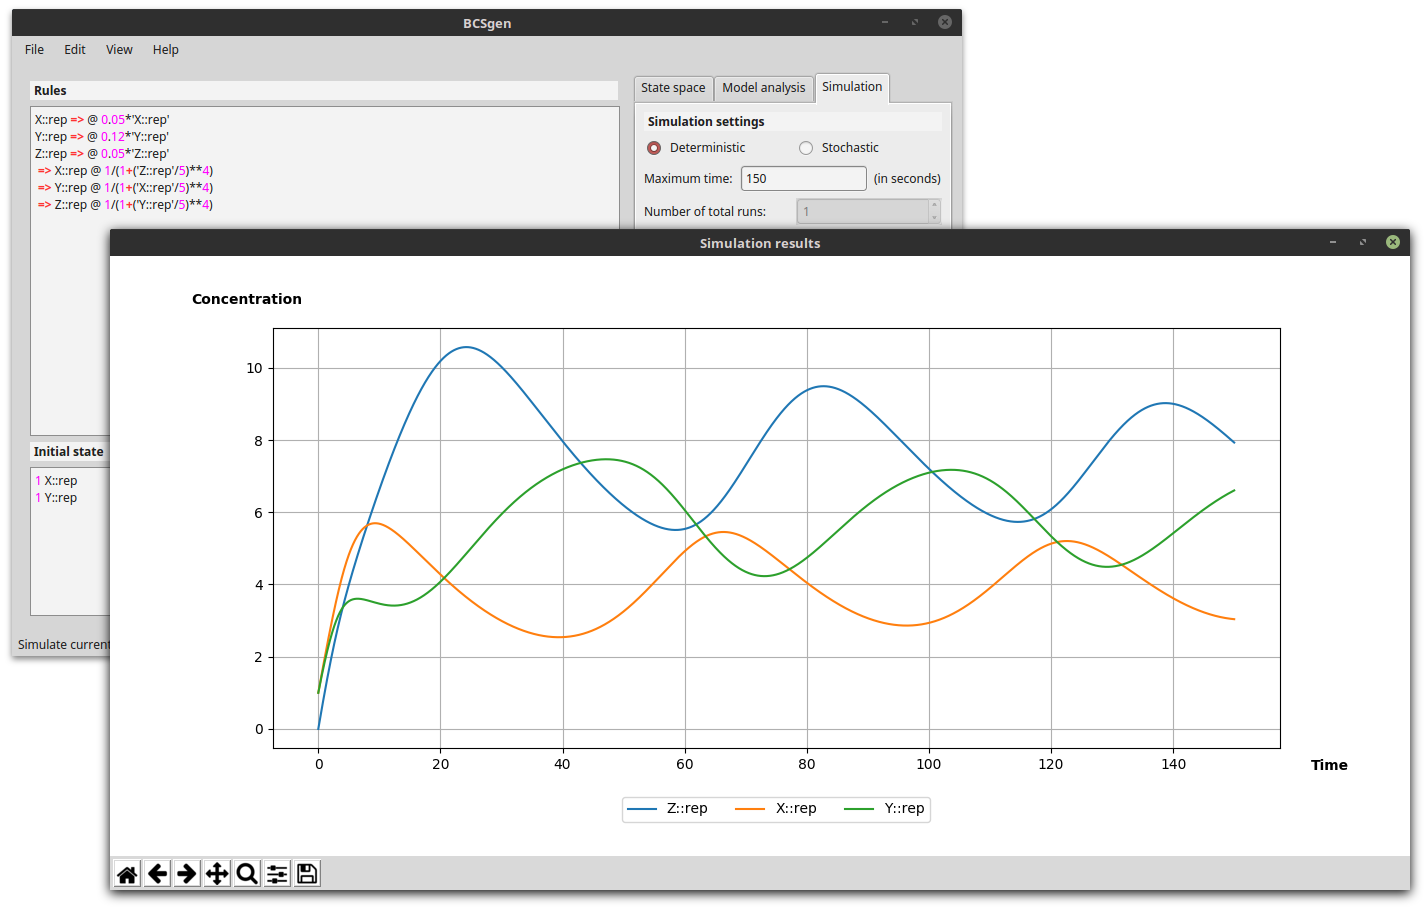
\includegraphics[scale=0.23]{pics/BCSgen_simulation}
\caption{Example of a deterministic simulation for simple repressilator model. For the simulation to be enabled, the rates for individual rules has to be defined. In the right panel, deterministic approach and the maximum simulation time is chosen.}\label{gui_simulation}
\end{center}
\end{figure}

Since there are some graphs and charts generated in BCSgen, we decided to integrate visualisation tools into it. We used two libraries -- vis.js~\cite{almende2016vis} for interactive networks visualisation and MatPlotLib~\cite{hunter2007matplotlib}, a Python library suitable for visualisation of time series.

Vis.js is used for exploration of state space with highlighting chosen node and announcing content of the node. It is possible to display paths from the initial state to other states, which satisfy reachability condition given in reachability analysis part (Figure~\ref{gui_reach}). This is very demonstrative and suitable for educational purposes. However, such visualisation has its limitations. For example, huge graphs are very difficult to display -- on the other hand, for a high number of nodes it is not even useful.

The MatPlotLib provides visualisation of simulation results. It possible to zoom the chart, hide/show individual curves, and export the current view as a picture.

\begin{figure}[!h]
\begin{center}
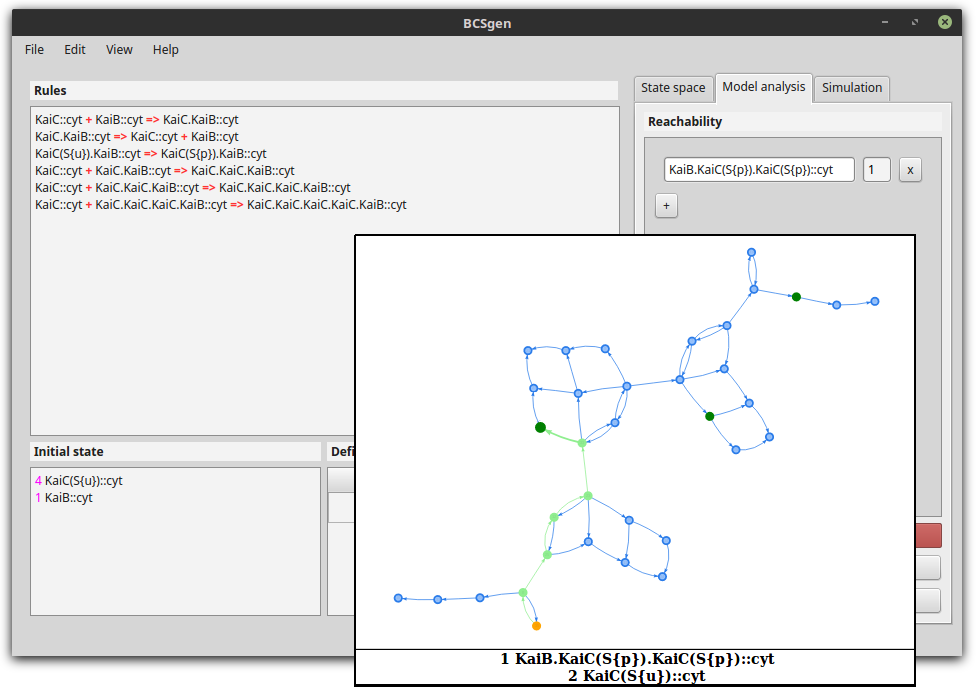
\includegraphics[scale=0.35]{pics/BCSgen_reach}
\caption{A graph showing LTS of given model. There are a few types of vertices in the graph: \textbf{orange} -- the initial state; \textbf{dark green} -- states satisfying condition given in right panel of the GUI; \textbf{bright green} -- path from initial to chosen reachable state.}\label{gui_reach}
\end{center}
\end{figure}

% \chapter{Discussion}

% \subsubsection{The difference between BCS and BCSL}

% It is important to realise the difference between Biochemical Space and Biochemical Space Language which we are about to define.

% The general goal of BCS is to provide knowledge base for mathematical models. In order to achieve that, Biochemical Space is formed by a database of biochemical entities. This allows us to describe particular objects with their attributes and properties and form space hierarchy. Each entity should be properly annotated by description and links to suitable external databases. However, entities are not enough for describing models since it requires also process hierarchy. Therefore, alongside with space hierarchy of entities, process hierarchy is build via interactive schemes. The hierarchy allows us to zoom on individual rules which present atomic operations happening on the entities.

% To improve usability and verifiability of the BCS, we define Biochemical Space Language. The language formally describes the entities and the rules. It has rule-based semantics, what allows compact description of the objects. Moreover, the syntax was designed in order to be very concise and human-readable. Hence it is very suitable for our needs.

% The whole BCS is defined in BCSL. This fact makes sure the entities and the rules are defined with all appropriate properties. Moreover, it helps us to relate objects from the models to BCS objects. Note that due to rule-based nature of the BCSL, in BCS there are defined only abstract objects representing types. Therefore, when relating for example an model variable to BCS entity, we might need to specify its properties. 

% \begin{figure}[!h]
% \begin{center}
%   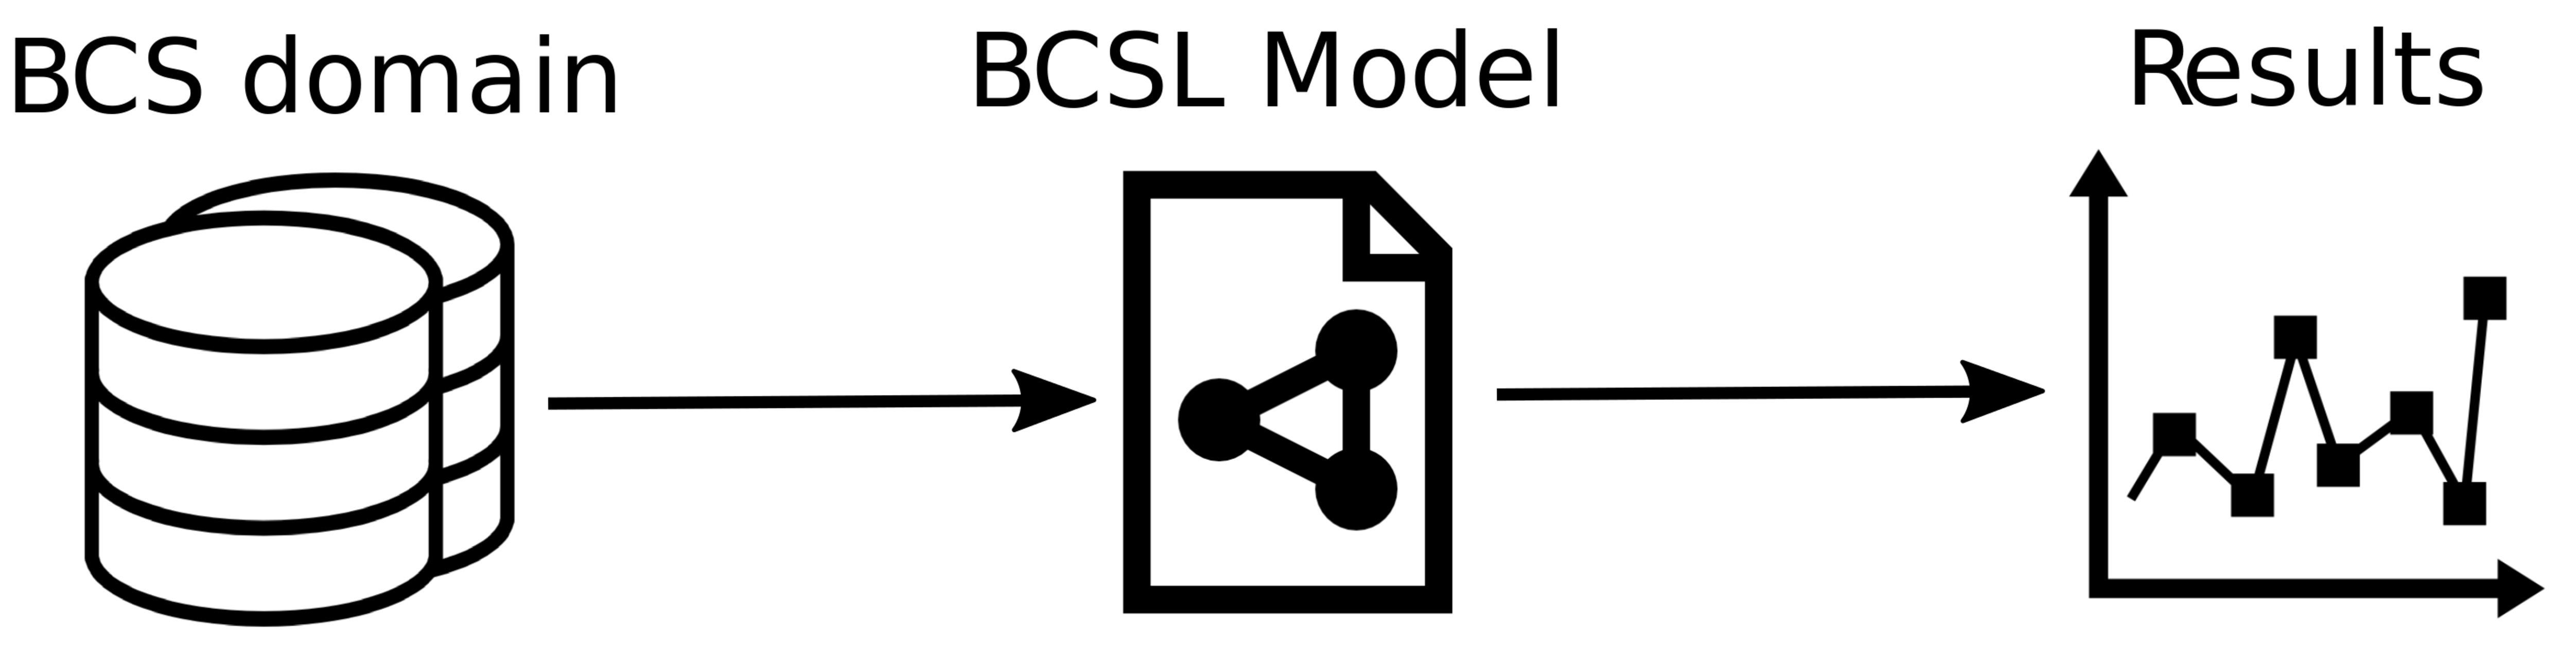
\includegraphics[scale=0.13]{pics/bcsl_vs_bcs.pdf}
% \end{center}
% \caption{BCS domain serves for improved BCSL models definition, which leads to better model readability and results.}
% \end{figure}

% Once BCS is build, we can use it to reference the models. It means to relate all the variables and reactions of the model and to entities and rules of BCS. In particular, each variable should have assigned an entity for BCS. It increases information value of the variable (due to annotation of BCS entity). Since reactions of the model are composed from its variables, this way we also rewrite general reactions to reactions written in BCSL. The result of relating all the entities is model written in BCSL. 

% Model defined in BCSL has two main advantages -- formal analysis can be applied on the model and the biological meaning of the whole model is fully reconstructed.

% To sum it up, BCS serves as definition domain for models written in BCSL (so called signature). It defines what can and what cannot be written in models and also increases rule compactness due to syntactic extensions. For example, some context might be omitted from the rule because it can be reconstructed from the signature.

\chapter{Conclusions}

In the first part of this thesis, we have explained the background of the work. Particularly, we provided explanation of the principles of rule-based modelling using schematic examples. Several existing rule-based languages have been introduced with their key features. Comprehensive Modeling Platform as a framework for modelling biochemical processes has been described with all its important modules such as Model repository and Biochemical Space.

In the second part, we have formally defined Biochemical Space Language as a description format for Biochemical Space. Together with very concise and \emph{human-readable} syntax we have defined operational semantics. An indirect approach has been chosen for practical purposes. Moreover, several syntactic extensions were defined to increase readability and maintenance of the language.

In the third part, we have introduced analysing approaches which could be directly used on model defined using the language. Those include dynamic analyses such as model checking and simulation. We have also defined a few types of static analyses which can be use without enumerating entire behaviour of the model.

The last part was dedicated for practical usage of the language and provided analysis formalisms. Namely, in the case study we have demonstrated how can be abstractions of the language used in particular modelling situations. We have also shown practical impact of defined static analyses on investigating behaviour of the model effectively. Finally, we have presented implementation of a software tool BCSgen, which was developed in order to provide support for maintenance and analysis of the models.

As a future work, we want to improve specification of kinetic rates for the BCSL rules. In the current stage, we allow to reference only fully defined objects in the kinetic rates. This is a very limiting restriction, because it would be natural to change context in rate and the rule simultaneously.

The next goal for the future work is to make some of the static analyses more general. Particularly, some of non-reachability analyses were defined only for a single complex agent. We want to promote these analyses in order to be applied on sets (or multisets) of agents.

Finally, as a future work for the tool BCSgen we are planning to reimplement it to a web-based version. It should be integrated in Comprehensive Modeling Platform (Section~\ref{cmp}) to allow direct analysis of the models and appropriate parts of Biochemical Space. 

\bibliographystyle{citeStyle}
{\small
\bibliography{papers}
}

\appendix

\chapter{List of used notation}

\begin{center}
\begin{tabular}{c | l}
$\sigma(\vv{v})$ & set of permutations of vector $\vv{v}$ of length $|\vv{v}|$\\
$X \mdoubleplus Y$ & tuples concatenation\\
$\mdoubleplus_{i=1}^n T_i$ & generalised concatenation\\
$\Xi(Y)$ & reassembly of tuples\\
$\pi_i$ & projection on dimension i\\
\hline 
$\Sigma_{\mathtt{A}}$ & atomic signature \\
$\Sigma_{\mathtt{T}}$ & structure signature \\
\hline 
$\mathtt{A}$ & atomic agent \\
$\eta$ & name \\
$\delta$ & state \\
$\varepsilon$ & empty state (not specified)\\
$\mathds{A}$ & universe of all possible atomic agents \\
\hline 
$\mathtt{T}$ & structure agent \\
$\eta$ & name \\
$\gamma$ & partial composition\\
$\mathds{T}$ & universe of all possible structure agents\\
\hline 
$\mathtt{X}$ & complex agent\\
$\mu$ & sequence of agents\\
$\mathtt{com}$ & compartment\\
$\mathds{X}$ & universe of all possible complex agents\\
$\mathds{U}$ & universe of all possible agents\\
\hline 
$\mathtt{R}$ & rule\\
$\chi$ & sequence of complexes\\
$\omega$ & sequence of atomic and structure agents\\
$\iota$ & index determining start of right-hand side\\
$\varphi$ & index map between $\omega$ and $\chi$\\
$\psi$ & is an index map between agents from left-\\
 & and right-hand side\\
$\mathds{R}$ & universe of all possible rules\\
\hline 
$\mathtt{r}$ & reaction\\
$LHS(\mathtt{r})$ & left-hand side of the reaction\\
$RHS(\mathtt{r})$ & right-hand side of the reaction\\
\hline 
$\alpha$ & atomic expression\\
$\tau$ & structure expression\\
$\Gamma$ & complex expression\\
$\varrho$ & rule expression\\
$\beta$ & atomic or structure expression\\
\end{tabular}
\end{center}

\begin{center}
\begin{tabular}{c | l}
$\mathds{M}$ & BCSL model\\
$\mathcal{R}$ & set of rule expressions\\
$\mathtt{init}$ & initial multiset of complex expressions\\
\hline 
$\gamma \ominus \gamma'$ & difference of partial compositions\\
$\Sigma_T(\mathtt{\eta(\mathtt{T})}) \ominus \gamma(\mathtt{T})$ & difference of partial composition and\\
 & structure signature\\
 \hline 
$\mathtt{F}$ & semantic function\\
$\mathcal{G}$ & ground form function\\
\hline 
$\mathcal{M}$ & Chemical reaction model\\
$\mathfrak{R}$ & set of chemical reactions\\
$\vv{\nu}$ & initial vector\\
$\theta$ & vector of reference complexes\\
\hline 
$\zeta$ & chemical reaction application\\
$\mathtt{S}$ & a multiset of agents\\
$\lambda(\mathtt{S}, \theta)$ & multiset to vector translation\\
\end{tabular}
\end{center}

% \chapter{Discussion about rates and how they could be solved}
% \label{rates_discussion}

% In order to provide numerical simulation, we need to assign a reaction rate to each rule. However, this is quite a challenging task and we will briefly explain why.

% The general problem is that typical kinetic rules in biology require usage of concentration of an agent in volume of the system. This is often solved via absolute numbers (the number of repetitions). The number might be either natural number of we are working with stochastic simulation or even real number if we compute average traces such as in deterministic simulation (make this more precise with citations!!!).

% Compared to reaction-based models, we work with fully defined objects which we can simply reference in the kinetics without any limitations. We can do the very same in rule-based models, but it is not desired solution. The thing is we would like to express the context of the rule also in the kinetics. That typically means when context in which the rule is being applied changes, we want appropriate change in the kinetics. To make this more clear, we provide an example.

% Example goes here...

% There are several solutions of this problem. However, none of them is an optimal one and therefore this remains an open problem. In other languages... they solved it as... finish this...

% Another general problem which causes issues is stoichiometry. The problem is if we reference an agent which has multiple enumerations in the rule, it is not clear which one should be used as reference in kinetics. Therefore we distinguish two types of solutions:

% \textbf{Solutions with forbidden stoichiometry}:

% \begin{enumerate}
% \item unique agents

% In this case, we allow arbitrary kinetics, but with a restriction. It is not allowed to use two identical agents in the same rule (including both sides of the rule). Moreover, in kinetics it is allowed to use only agents which are already used in the rule (in the very same form). This restriction decreases the expressiveness of the rules -- for example, it is not possible to define agents which are required but not consumed in the rule. However, mapping between agents in rule and kinetics are clear.

% \item almost optimal solution

% In order to make sure the agent from kinetics and rule are connected properly, we would have to extend the syntax of the language itself. For example, and agent might be enriched by `$\sim\mathbb{N}$' in both places. Then, the mapping would be unambiguous. However, such s syntax extension leads to decreases readability of the language, which definitely not desired solution. Optionally, the numbering of agents might be implicit, what does not change syntax of the language, but makes it harder to write w.r.t. language simplicity.

% \end{enumerate}


% \textbf{Solutions with allowed stoichiometry}:

% \begin{enumerate}
% \item we allow only \emph{mass action} kinetics

% The positive thing about this kinetics is that all it needs is a given parameter. The rate is computed as multiple of the parameter with all agents on the left-hand side of the rule. Since the stoichiometry is allowed in this case, the mapping is not always clear. For this reason we multiply all possible mappings together, which gives appropriate results.

% \item the first left agent

% Arbitrary kinetics might be used, but both rule and kinetics must be defined very carefully. The method for mapping rate agent to rule agent is very simple -- whenever an agent is referenced in kinetics, first suitable rule-agent from the left is chosen. This solution is very simple to use, but rules are not that easy to write.

\chapter{Model Yamada et al. 2004}
\label{yamada_complete}

\begin{figure}[!h]
{\tiny
\begin{center}
\begin{tabular}{ r c l }
$FGF::cyt + R::cyt $ & $\Leftrightarrow$ & $ FGF.R::cyt$\\
$2~ FGF.R::cyt $ & $\Leftrightarrow$ & $ FGF.R.FGF.R::cyt$\\
$FGF(Thr\{u\}).R.FGF.R::cyt $ & $\Leftrightarrow$ & $ FGF(Thr\{p\}).R.FGF.R::cyt$\\
$FRS(Thr\{u\})::cyt + FGF(Thr\{p\}).R.FGF(Thr\{p\}).R::cyt $ & $\Rightarrow$ & $ FGF(Thr\{p\}).R.FGF(Thr\{p\}).R.FRS(Thr\{u\})::cyt$\\
$FRS(Thr\{u\}).FGF.R.FGF.R::cyt $ & $\Rightarrow$ & $ FRS(Thr\{p\}).FGF.R.FGF.R::cyt$\\
$FRS(Thr\{p\}).FGF.R.FGF.R::cyt $ & $\Rightarrow$ & $ FRS(Thr\{p\})::cyt + FGF.R.FGF.R::cyt$\\
$FRS(Thr\{p\})::cyt + SHP::cyt $ & $\Rightarrow$ & $ SHP.FRS(Thr\{p\})::cyt$\\
$FRS(Thr\{p\}).SHP::cyt $ & $\Rightarrow$ & $ FRS(Thr\{u\}).SHP::cyt$\\
$FRS(Thr\{u\}).SHP::cyt $ & $\Rightarrow$ & $ FRS(Thr\{u\})::cyt + SHP::cyt$\\
$GS(Thr\{p\})::cyt + GPP::cyt $ & $\Rightarrow$ & $ GPP.GS(Thr\{p\})::cyt$\\
$GS(Thr\{p\}).GPP::cyt $ & $\Rightarrow$ & $ GS(Thr\{u\}).GPP::cyt$\\
$GS(Thr\{u\}).GPP::cyt $ & $\Rightarrow$ & $ GS(Thr\{u\})::cyt + GPP::cyt$\\
$GS(Thr\{u\})::cyt + ERK(Tyr\{p\},Thr\{p\})::cyt $ & $\Rightarrow$ & $ ERK(Tyr\{p\},Thr\{p\}).GS(Thr\{u\})::cyt$\\
$GS(Thr\{u\}).ERK::cyt $ & $\Rightarrow$ & $ GS(Thr\{p\}).ERK::cyt$\\
$GS(Thr\{p\}).ERK::cyt $ & $\Rightarrow$ & $ GS(Thr\{p\})::cyt + ERK::cyt$\\
$FRS(Thr\{p\},Tyr\{u\})::cyt + GS(Thr\{u\})::cyt $ & $\Leftrightarrow$ & $ FRS(Thr\{p\},Tyr\{u\}).GS(Thr\{u\})::cyt$\\
$Ras(Thr\{u\})::cyt + FRS(Thr\{p\},Tyr\{u\}).GS(Thr\{u\})::cyt $ & $\Rightarrow$ & $ FRS(Thr\{p\},Tyr\{u\}).GS(Thr\{u\}).Ras(Thr\{u\})::cyt$\\
$Ras(Thr\{u\}).FRS.GS::cyt $ & $\Rightarrow$ & $ Ras(Thr\{p\}).FRS.GS::cyt$\\
$Ras(Thr\{p\}).FRS.GS::cyt $ & $\Rightarrow$ & $ Ras(Thr\{p\})::cyt + FRS.GS::cyt$\\
$Ras(Thr\{p\})::cyt + GAP::cyt $ & $\Rightarrow$ & $ GAP.Ras(Thr\{p\})::cyt$\\
$Ras(Thr\{p\}).GAP::cyt $ & $\Rightarrow$ & $ Ras(Thr\{u\}).GAP::cyt$\\
$Ras(Thr\{u\}).GAP::cyt $ & $\Rightarrow$ & $ Ras(Thr\{u\})::cyt + GAP::cyt$\\
$Raf(Thr\{u\})::cyt + Ras(Thr\{p\})::cyt $ & $\Rightarrow$ & $ Ras(Thr\{p\}).Raf(Thr\{u\})::cyt$\\
$Raf(Thr\{u\}).Ras::cyt $ & $\Rightarrow$ & $ Raf(Thr\{p\}).Ras::cyt$\\
$Raf(Thr\{p\}).Ras::cyt $ & $\Rightarrow$ & $ Raf(Thr\{p\})::cyt + Ras::cyt$\\
$Raf(Thr\{p\})::cyt + PP::cyt $ & $\Rightarrow$ & $ PP.Raf(Thr\{p\})::cyt$\\
$Raf(Thr\{p\}).PP::cyt $ & $\Rightarrow$ & $ Raf(Thr\{u\}).PP::cyt$\\
$Raf(Thr\{u\}).PP::cyt $ & $\Rightarrow$ & $ Raf(Thr\{u\})::cyt + PP::cyt$\\
$MEK(Ser212\{u\})::cyt + Raf(Thr\{p\})::cyt $ & $\Rightarrow$ & $ Raf(Thr\{p\}).MEK(Ser212\{u\})::cyt$\\
$MEK(Ser212\{u\}).Raf::cyt $ & $\Rightarrow$ & $ MEK(Ser212\{p\}).Raf::cyt$\\
$MEK(Ser212\{p\}).Raf::cyt $ & $\Rightarrow$ & $ MEK(Ser212\{p\})::cyt + Raf::cyt$\\
$MEK(Ser298\{u\})::cyt + Raf(Thr\{p\})::cyt $ & $\Rightarrow$ & $ Raf(Thr\{p\}).MEK(Ser298\{u\})::cyt$\\
$MEK(Ser298\{u\}).Raf::cyt $ & $\Rightarrow$ & $ MEK(Ser298\{p\}).Raf::cyt$\\
$MEK(Ser298\{p\}).Raf::cyt $ & $\Rightarrow$ & $ MEK(Ser298\{p\})::cyt + Raf::cyt$\\
$MEK(Ser212\{p\})::cyt + XPP::cyt $ & $\Rightarrow$ & $ XPP.MEK(Ser212\{p\})::cyt$\\
$MEK(Ser212\{p\}).XPP::cyt $ & $\Rightarrow$ & $ MEK(Ser212\{u\}).XPP::cyt$\\
$MEK(Ser212\{u\}).XPP::cyt $ & $\Rightarrow$ & $ MEK(Ser212\{u\})::cyt + XPP::cyt$\\
$MEK(Ser298\{p\})::cyt + XPP::cyt $ & $\Rightarrow$ & $ XPP.MEK(Ser298\{p\})::cyt$\\
$MEK(Ser298\{p\}).XPP::cyt $ & $\Rightarrow$ & $ MEK(Ser298\{u\}).XPP::cyt$\\
$MEK(Ser298\{u\}).XPP::cyt $ & $\Rightarrow$ & $ MEK(Ser298\{u\})::cyt + XPP::cyt$\\
$ERK(Thr\{u\})::cyt + MEK(Ser212\{p\},Ser298\{p\})::cyt $ & $\Rightarrow$ & $ MEK(Ser212\{p\},Ser298\{p\}).ERK(Thr\{u\})::cyt$\\
$ERK(Thr\{u\}).MEK::cyt $ & $\Rightarrow$ & $ ERK(Thr\{p\}).MEK::cyt$\\
$ERK(Thr\{p\}).MEK::cyt $ & $\Rightarrow$ & $ ERK(Thr\{p\})::cyt + MEK::cyt$\\
$ERK(Tyr\{u\})::cyt + MEK(Ser212\{p\},Ser298\{p\})::cyt $ & $\Rightarrow$ & $ MEK(Ser212\{p\},Ser298\{p\}).ERK(Tyr\{u\})::cyt$\\
$ERK(Tyr\{u\}).MEK::cyt $ & $\Rightarrow$ & $ ERK(Tyr\{p\}).MEK::cyt$\\
$ERK(Tyr\{p\}).MEK::cyt $ & $\Rightarrow$ & $ ERK(Tyr\{p\})::cyt + MEK::cyt$\\
$ERK(Thr\{p\})::cyt + MKP::cyt $ & $\Rightarrow$ & $ MKP.ERK(Thr\{p\})::cyt$\\
$ERK(Thr\{p\}).MKP::cyt $ & $\Rightarrow$ & $ ERK(Thr\{u\}).MKP::cyt$\\
$ERK(Thr\{u\}).MKP::cyt $ & $\Rightarrow$ & $ ERK(Thr\{u\})::cyt + MKP::cyt$\\
$ERK(Tyr\{p\})::cyt + MKP::cyt $ & $\Rightarrow$ & $ MKP.ERK(Tyr\{p\})::cyt$\\
$ERK(Tyr\{p\}).MKP::cyt $ & $\Rightarrow$ & $ ERK(Tyr\{u\}).MKP::cyt$\\
$ERK(Tyr\{u\}).MKP::cyt $ & $\Rightarrow$ & $ ERK(Tyr\{u\})::cyt + MKP::cyt$\\
$FRS(Tyr\{u\})::cyt + ERK(Tyr\{p\},Thr\{p\})::cyt $ & $\Rightarrow$ & $ ERK(Tyr\{p\},Thr\{p\}).FRS(Tyr\{u\})::cyt$\\
$FRS(Tyr\{u\}).ERK::cyt $ & $\Rightarrow$ & $ FRS(Thr\{u\},Tyr\{p\}).ERK::cyt$\\
$FRS(Thr\{u\},Tyr\{p\}).ERK::cyt $ & $\Rightarrow$ & $ FRS(Thr\{u\},Tyr\{p\})::cyt + ERK::cyt$\\
$FRS(Tyr\{p\})::cyt $ & $\Rightarrow$ & $ FRS(Tyr\{u\})::cyt$\\
\end{tabular}
\end{center}
}
\caption{A complete model Yamada 2004~\cite{yamada2004model} of FGF signalling pathway written in BCSL. It consists of 20 entities interacting in 56 rules. To have this model complete, initial state has to be defined -- particularly, all entities have their subparts in unphosphorylated state and each of them is present once but $FGF$ and $R$ are present in two repetitions.}
\end{figure}

\end{document}
